% CVPR 2025 Paper Template; see https://github.com/cvpr-org/author-kit

\documentclass[10pt,twocolumn,letterpaper]{article}

%%%%%%%%% PAPER TYPE  - PLEASE UPDATE FOR FINAL VERSION
% \usepackage{cvpr}              % To produce the CAMERA-READY version
\usepackage{cvpr}      % To produce the REVIEW version
% \usepackage[pagenumbers]{cvpr} % To force page numbers, e.g. for an arXiv version

% Import additional packages in the preamble file, before hyperref
%
% --- inline annotations
%
\newcommand{\red}[1]{{\color{red}#1}}
\newcommand{\todo}[1]{{\color{red}#1}}
\newcommand{\TODO}[1]{\textbf{\color{red}[TODO: #1]}}
% --- disable by uncommenting  
% \renewcommand{\TODO}[1]{}
% \renewcommand{\todo}[1]{#1}

%%%%%%%%%%%
\usepackage{booktabs}
\usepackage{multirow}
\usepackage{adjustbox}
\usepackage{tabularx, colortbl}
\usepackage{bbding}
%\usepackage{hyperref}       % hyperlinks
\usepackage{url}            % simple URL typesetting
\usepackage{booktabs}       % professional-quality tables
\usepackage{amsfonts}       % blackboard math symbols
\usepackage{nicefrac}       % compact symbols for 1/2, etc.
\usepackage{microtype}      % microtypography
\usepackage{xcolor}         % colors
\usepackage{amsmath}
\usepackage{amssymb}
\usepackage{enumitem}
\usepackage{amsthm}

%%%%%%%%%%%
\newtheorem{theorem}{Theorem}
\newtheorem{lemma}{Lemma}
\newtheorem{assumption}{Assumption}
\newtheorem{proposition}{Proposition}

%%%%%%%%%%%
\DeclareMathOperator{\x}{\mathbf{x}}
\DeclareMathOperator{\Phix}{\mathbf{\Phi x}}
\DeclareMathOperator{\y}{\mathbf{y}}
\DeclareMathOperator{\PhiTy}{\mathbf{\Phi}^T \mathbf{y}}
\DeclareMathOperator{\PhiTu}{\mathbf{\Phi}^T \mathbf{u}}
\DeclareMathOperator{\bfPhi}{\mathbf{\Phi}}
\DeclareMathOperator{\bfA}{\mathbf{A}}
\DeclareMathOperator{\bfW}{\mathbf{W}}
\DeclareMathOperator{\R}{\mathbb{R}}
\DeclareMathOperator{\I}{\mathbf{I}}
\DeclareMathOperator{\zz}{\mathbf{z}}
\DeclareMathOperator{\rr}{\mathbf{r}}
\DeclareMathOperator{\bb}{\mathbf{b}}
\DeclareMathOperator{\bfs}{\mathbf{s}}
\DeclareMathOperator{\hh}{\mathbf{h}}
\DeclareMathOperator{\bfu}{\mathbf{u}}
\DeclareMathOperator{\barAlpha}{\bar{\alpha}}
\DeclareMathOperator{\bfd}{\mathbf{d}}


% It is strongly recommended to use hyperref, especially for the review version.
% hyperref with option pagebackref eases the reviewers' job.
% Please disable hyperref *only* if you encounter grave issues, 
% e.g. with the file validation for the camera-ready version.
%
% If you comment hyperref and then uncomment it, you should delete *.aux before re-running LaTeX.
% (Or just hit 'q' on the first LaTeX run, let it finish, and you should be clear).
\usepackage{colortbl}
\definecolor{cvprblue}{rgb}{0.21,0.49,0.74}
\usepackage[pagebackref,breaklinks,colorlinks,allcolors=cvprblue]{hyperref}
\usepackage{multirow}
\usepackage{pdflscape} % landscape page
\usepackage{changepage} % move table left via adjustwidth
\usepackage[export]{adjustbox}
\usepackage{array}
\usepackage{booktabs}
\usepackage{graphicx} 
% \usepackage{emoji}
% \usepackage[table]{xcolor}
\definecolor{lightblue}{RGB}{189, 224, 254}
%%%%%%%%% PAPER ID  - PLEASE UPDATE
\def\paperID{***} % *** Enter the Paper ID here  % Remeber remove this line for arxiv source
\def\confName{ICCV}
\def\confYear{2025}

\makeatletter
\AtBeginDocument{
\renewcommand{\sectionautorefname}{\S\@gobble}
\renewcommand{\tableautorefname}{Table}
\renewcommand{\equationautorefname}{Equation}
\renewcommand{\subsectionautorefname}{\S\@gobble} 
\renewcommand{\subsubsectionautorefname}{\S\@gobble}
\renewcommand{\appendixautorefname}{\S\@gobble}
\providecommand{\algorithmautorefname}{Algorithm}
}
\makeatother

%%%%%%%%% TITLE - PLEASE UPDATE
\title{MIEB: Massive Image Embedding Benchmark}

%%%%%%%%% AUTHORS - PLEASE UPDATE
\author{\textbf{Chenghao Xiao\textsuperscript{1,\textdagger}} \ \ 
\textbf{Isaac Chung\textsuperscript{2}}\ \ 
\textbf{Imene Kerboua\textsuperscript{3,4}} \ \ 
\textbf{Jamie Stirling\textsuperscript{1}}
\\
\textbf{Xin Zhang\textsuperscript{5}} \ \  
\textbf{Márton Kardos\textsuperscript{6}} \ \ 
\textbf{Roman Solomatin\textsuperscript{7}}
\\
\textbf{Noura Al Moubayed\textsuperscript{1}} \ \  
\textbf{Kenneth Enevoldsen\textsuperscript{6}} \ \
\textbf{Niklas Muennighoff \textsuperscript{8,9}}
\\ \\
\textsuperscript{1}Durham University,
\textsuperscript{2}Zendesk, 
\textsuperscript{3}Esker, 
\textsuperscript{4}INSA Lyon, LIRIS, \\
\textsuperscript{5}The Hong Kong Polytechnic University, 
\textsuperscript{6}Aarhus University, \\
\textsuperscript{7}ITMO University, 
\textsuperscript{8}Contextual AI, 
\textsuperscript{9}Stanford University
\\ 
\\
{\textsuperscript{\textdagger}Correspondence: \tt chenghao.xiao@durham.ac.uk}
}


\begin{document}

\maketitle

\begin{abstract}
Image representations are often evaluated through disjointed, task-specific protocols, leading to a fragmented understanding of model capabilities. For instance, it is unclear whether an image embedding model adept at clustering images is equally good at retrieving relevant images given a piece of text. We introduce the Massive Image Embedding Benchmark (MIEB) to evaluate the performance of image and image-text embedding models across the broadest spectrum to date. MIEB spans 38 languages across 130 individual tasks, which we group into 8 high-level categories. We benchmark 50 models across our benchmark, finding that no single method dominates across all task categories. We reveal hidden capabilities in advanced vision models such as their accurate visual representation of texts, and their yet limited capabilities in interleaved encodings and matching images and texts in the presence of confounders. We also show that the performance of vision encoders on MIEB correlates highly with their performance when used in multimodal large language models. Our code, dataset, and leaderboard are publicly available at \url{https://github.com/embeddings-benchmark/mteb}.
\end{abstract}

\section{Introduction}
\label{sec:intro}

\begin{figure*}[t]
\centering
\resizebox{\linewidth}{!}{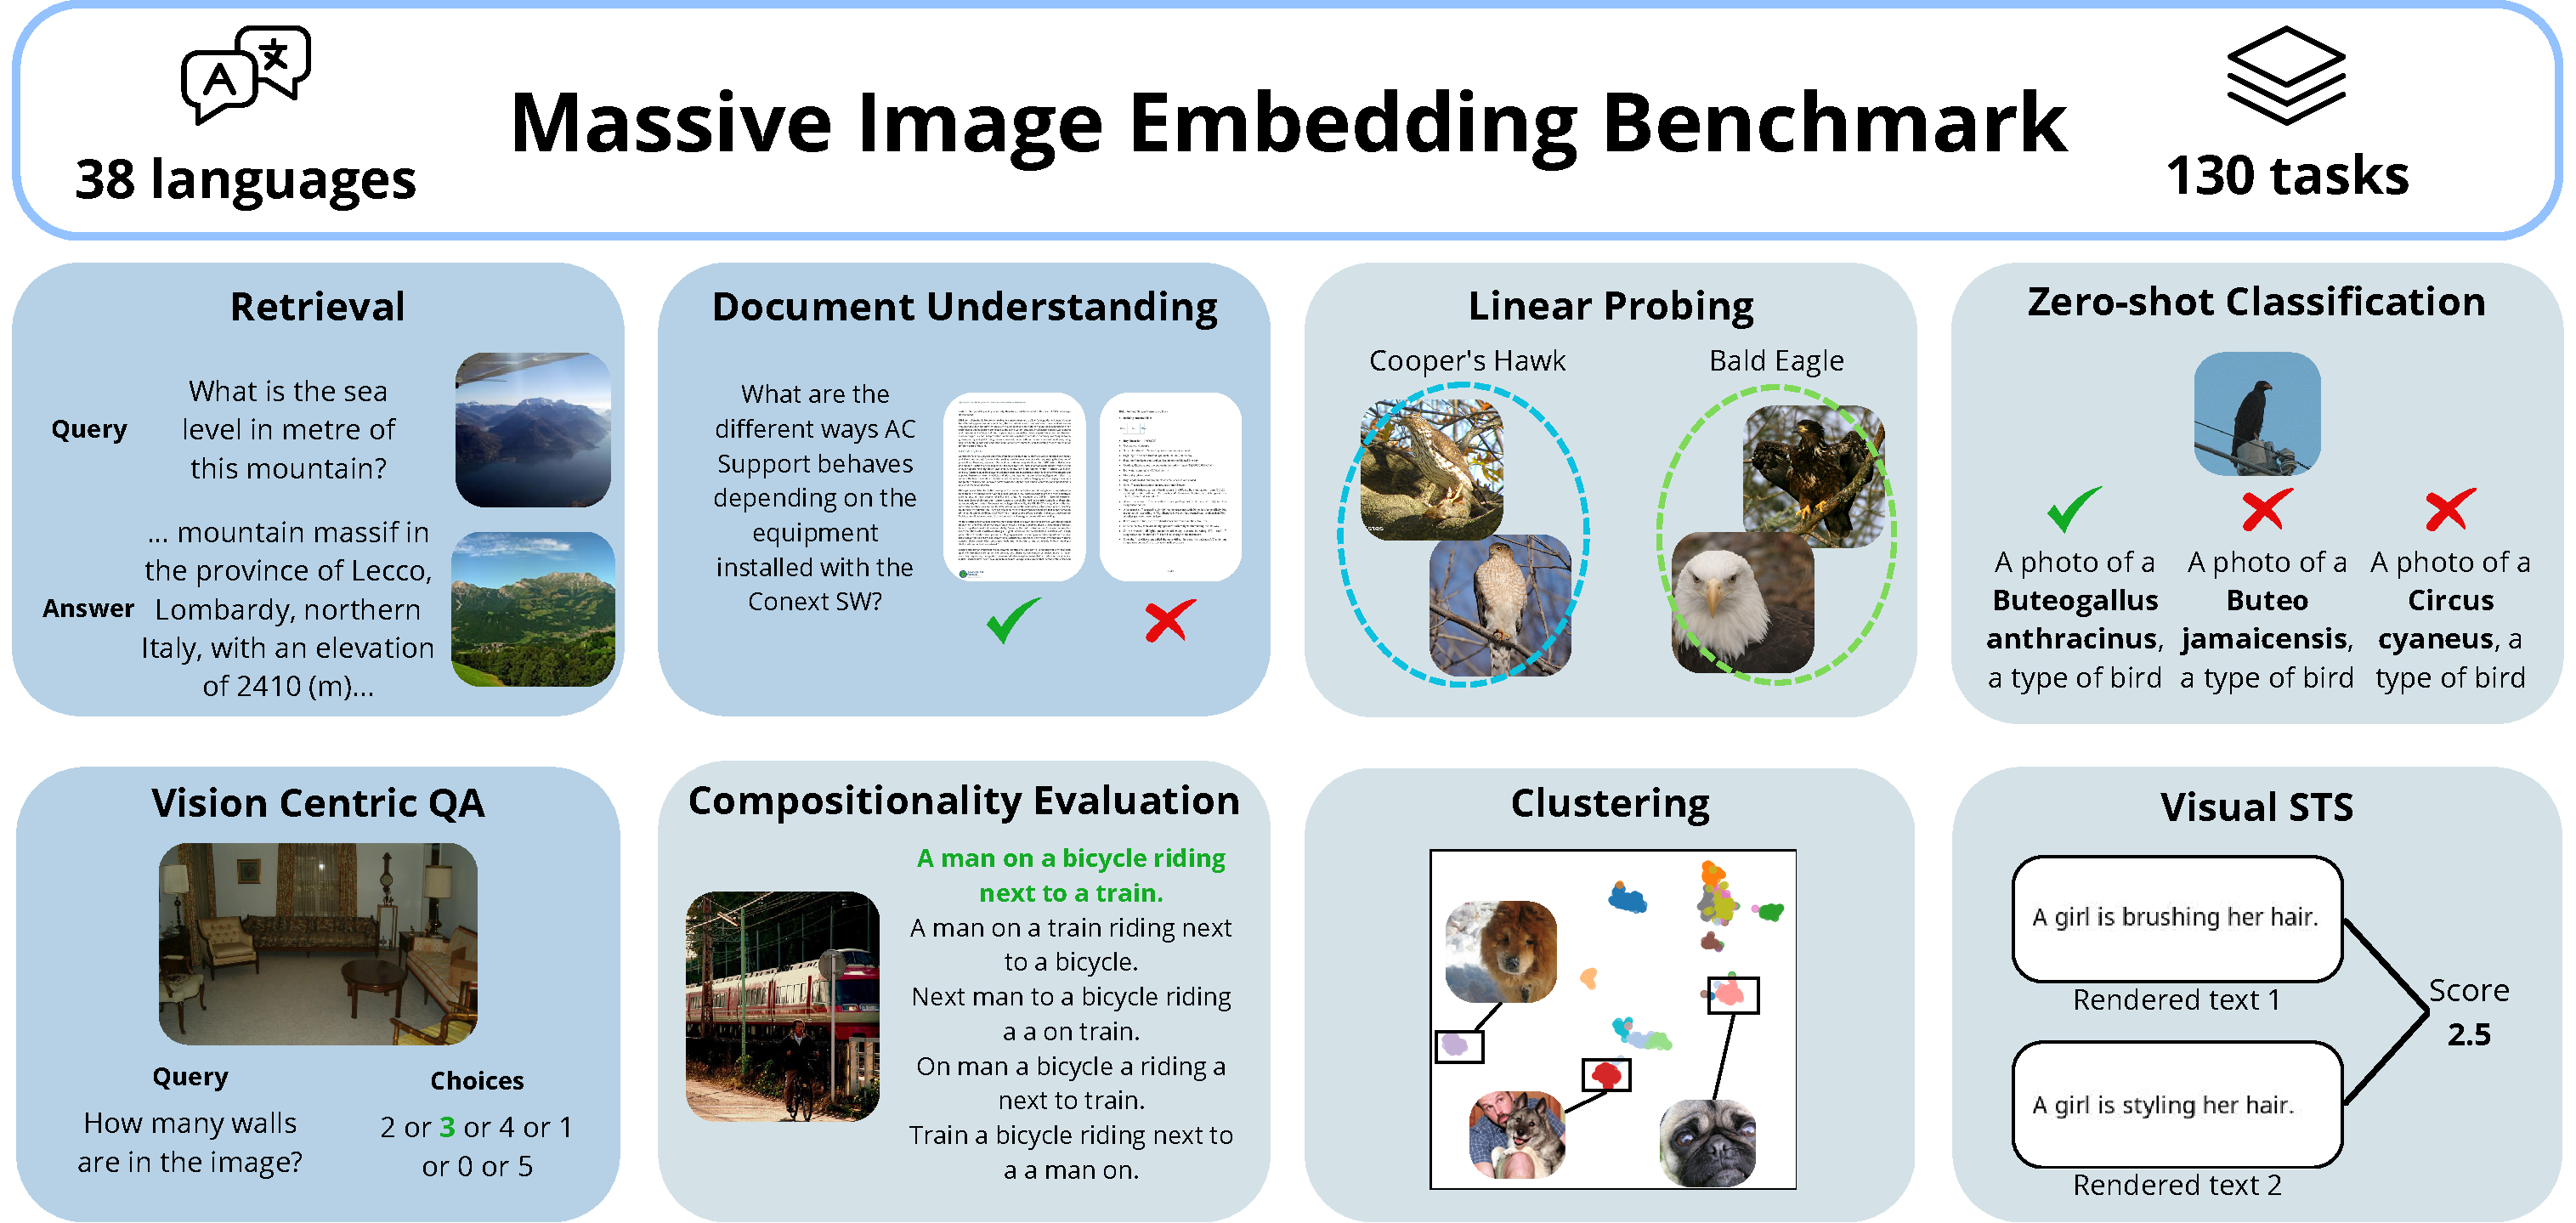
\includegraphics[width=\linewidth]{figures/MIEB_backup.pdf}}
\caption{\textbf{Overview of MIEB task categories with examples.} See \autoref{tab:MIEB big tasks} for details about capabilities measured and other information.} 
\label{fig:mieb_tasks}
\end{figure*}

Image and text embeddings power a wide range of use cases, from search engines to recommendation systems~\citep{geng2015learning,pinterest,huang2020embedding}. However, evaluation protocols for image and multimodal embedding models vary widely, ranging from image-text retrieval, zero-shot classification \citep{radford2021learning,zhai2023sigmoid}, linear probing \citep{radford2021learning,oquab2024dinov2}, fine-tuning the models \cite{chen2020simclr,he2019moco}, and using MLLM performance as proxies \cite{tong2024cambrian}.  These divergent protocols reveal the lack of standardized criteria for assessing image representations.

We introduce the Massive Image Embedding Benchmark (MIEB) to provide a unified comprehensive evaluation protocol to spur the field's advancement toward universal image-text embedding models. We build on the standard for the evaluation of text embeddings, MTEB~\citep{muennighoff2023mteb}, extending its codebase and leaderboard for image and image-text embedding models. MIEB spans 130 tasks grouped into 8 task categories: Aligning with MTEB, we integrate \textbf{Clustering}, \textbf{Classification}, and \textbf{Retrieval}. Notably, we consider fine-grained aspects, such as \textit{interleaved retrieval}, \textit{multilingual retrieval}, \textit{instruction-aware retrieval}. We additionally include \textbf{Compositionality Evaluation} and \textbf{Vision Centric Question Answering}, respectively assessing nuanced information encoded in embeddings and their capabilities in solving vision-centric QA tasks. We focus on tasks that require strong \textit{visual understanding of texts}, for which we include \textbf{Visual STS}, the visual counterpart of semantic textual similarity in NLP, and \textbf{Document Understanding}, assessing the vision-only understanding of high-resolution documents with dense texts and complex layout, enabling evaluation that pushes forward the development of natural interleaved embeddings.

Our analysis across task categories shows that the performance of current image embedding models is fragmented, with no method dominating all task categories. We further study the predictability of the performance of visual encoders as part of Multimodal Large Language Models (MLLMs), via a large-scale correlation study. We find that the performance of vision encoders on MIEB strongly correlates with the performance of MLLMs that use the same vision encoder. For instance, the performance on our Visual STS tasks has over 99\% correlation with the performance of an MLLM leveraging the same vision encoder on tasks like OCRBench and TextVQA. This provides a practical way to select vision encoders for MLLMs based on MIEB results. 

\section{The MIEB Benchmark}
\label{sec:mieb}

\begin{table*}[t]
\centering
\resizebox{\linewidth}{!}{
\begin{tabular}{lllcccc}
\toprule
\textbf{Task category} & \textbf{Example abilities assessed} & \textbf{\# Tasks} & \textbf{\# Languages} & \textbf{Modalities}\\
\midrule
\textbf{Retrieval} & cross-modal/-lingual matching & 45 & 38 & i-i; i-t; t-i; it-i; it-t; i-it; t-it; it-it; i-t \\
\textbf{Document Understanding (Retrieval)} & OCR abilities & 10 & 2 & t-i; i-t; it-t \\
\textbf{Linear Probing (Classification)} & information encoded & 22 & 1 & i-i; i-i \\
\textbf{Clustering} & embedding space consistency & 5 & 1 & i-i \\
\textbf{Zero-shot Classification} & cross-modal matching & 23 & 1 & i-t; i-t \\
\textbf{Compositionality Evaluation (PairClassification)} & reasoning with confounders & 7 & 1 & i-t; t-i \\
\textbf{Vision-centric QA (Retrieval)} & counting, object detection & 6 & 1 & it-t; it-i \\
\textbf{Visual STS} & OCR abilities & 9 & 12 & i-i \\
\midrule
\textbf{MIEB} & all & 130 & 38 & all \\
\textbf{MIEB-lite} & all & 51 & 38 & all \\
\bottomrule
\end{tabular}
}
\caption{\textbf{An overview of MIEB tasks.} In brackets behind task categories, we denote the task type implementation in the code, e.g., our document understanding tasks use our retrieval implementation. We denote the modalities involved in both sides of the evaluation (e.g., queries and documents in retrieval; images and labels in zero-shot classification) with i=image, t=text.
\label{tab:MIEB big tasks}}
\end{table*}

\subsection{Overview}

Existing image benchmarks are often task-specific (e.g., retrieval~\citep{wei2023uniir}) with fine-grained domains (e.g., landmarks~\citep{Weyand_2020_CVPR}, artworks~\citep{ypsilantis2021met}). MIEB provides a unified framework to evaluate diverse abilities of embedding models. We categorize tasks based on a combination of the evaluation protocol (e.g., Clustering) and the abilities assessed (e.g., Document Understanding) to better align with user interests. \autoref{fig:mieb_tasks} and \autoref{tab:MIEB big tasks} summarize MIEB task categories. Beyond traditional tasks like linear probing, zero-shot classification, and image-text retrieval, we emphasize under-explored capabilities in image-text embedding models via: \textbf{1)} Visual representation of texts, covered by document understanding and visual STS; \textbf{2)} Vision-centric abilities, including spatial and depth relationships; \textbf{3)} Compositionality; \textbf{4)} Interleaved embedding; \textbf{5)} Multilinguality.

In addition to MIEB (130 tasks), we introduce MIEB-lite, a lightweight version of MIEB with 51 tasks to support efficient evaluation, by selecting representative tasks from task performance clusters, detailed in \autoref{sec: MIEB-lite}. We refer to \autoref{sec:overview} for all datasets, statistics, and evaluation metrics for MIEB and MIEB-lite, and \autoref{sec:imp} for implementation details. Here, we discuss task categories and capabilities assessed.

\paragraph{Retrieval} Retrieval evaluates if embeddings of two similar items (images or texts) have high similarity~\citep{datta2008image}. We focus on three retrieval aspects: \textbf{1) Modality}: The combination of images and texts among queries and documents and whether they are interleaved; \textbf{2) Multilinguality}: Whether tasks cover mulitple languages, including texts in images; \textbf{3) Instructions} Some tasks may benefit from instructions on what to retrieve, e.g., in VQA tasks questions in the text serve as example-specific instructions. We use nDCG@10 as the primary metric~\citep{thakur2021beir,wei2023uniir}, and recall@1/map@5 for some tasks to align with prior work or adjust for difficulty.

\paragraph{Document understanding} There has been much interest in using image embeddings to understand entire documents with interleaved figures and tables~\citep{faysse2024colpali}. To address these needs, we create a separate document understanding category. It uses the same evaluation procedure as retrieval and nDCG@5 as the main metric.

\paragraph{Linear probing} For linear probing, a linear model is trained on embedded images to predict associated class labels~\citep{alain2018understandingintermediatelayersusing,radford2021learning}. Linear probing allows evaluating knowledge encoded in embeddings, even if they are not spatially consistent as would be needed for good clustering performance. We opt for few-shot linear probing~\citep{muennighoff2023mteb,cherti2023reproducible} with a default of 16 shots per class on which we train a logistic regression classifier with a maximum of 100 iterations. This method is more efficient than probing on the entire dataset~\citep{chen2021empirical,radford2021learning,oquab2024dinov2}, making it suitable for large-scale benchmarks like ours. In \autoref{subsec: k-shot}, we ablate the performance trend of k-shot per class, showing that model ranking generally remains the same across different values of k. In text embeddings, this task is often called classification~\citep{muennighoff2023mteb}, so we adopt that term in our code.

\paragraph{Zero-shot Classification} While generally using the same tasks as linear probing (e.g.,  ImageNet~\citep{deng2009imagenet}), zero-shot Classification directly matches image embeddings to classes without training a separate classifier. We follow common practice and turn class labels into text prompts (e.g., for our ImageNet task, a text prompt could be ``a photo of space shuttle''). This task is related to retrieval, specifically, a setting where we only care about the top-1 match. We measure accuracy following prior work~\citep{radford2021learning}. Models trained with non-representation losses, such as autoregressive models, often lack good off-the-shelf zero-shot performance, but may still perform well in linear probing~\citep{reimers2019sentence}.

\paragraph{Compositionality Evaluation} Vision-language compositionality assesses whether the composition of a given set of elements aligns with an image and a text, such as relationships between objects, attributes, and spatial configurations. Commonly, it involves distinguishing a ground truth from hard negatives with perturbed inputs, e.g., word order shuffling in ARO benchmark \cite{yuksekgonul2023aro}. In our code implementation, we also refer to it as ImageTextPairClassification, as images and texts come in small pairs. The main metric we use for this task category is accuracy.

\paragraph{Vision-centric question answering} Inspired by insights from MLLMs~\citep{tong2024cambrian}, we include vision centric question answering tasks, including object counting, spatial relationships, etc. We also include other challenging visual perception tasks, such as perceiving art styles. This task category can be seen as a form of retrieval where the corpus is a small set of query-specific options (see \autoref{fig:mieb_tasks}), thus it uses our retrieval code implementation.

\paragraph{Clustering} We use k-means clustering (with k set to the number of true labels) and Normalized Mutual Information (NMI)~\citep{collignon1995automated,studholme1999overlap} as the main metric to evaluate if image embeddings group meaningfully in the embedding space according to the labels.

\paragraph{Visual STS} Semantic textual similarity (STS) is an established task to evaluate text embeddings~\cite{agirre-etal-2013-sem,cer-etal-2017-semeval}. It measures the similarity of text embeddings compared to human annotations via Spearman correlation.

In MIEB, we conceptualize \textit{``Visual STS"}~\citep{xiao2024pixel} as an out-of-distribution task to assess \textit{how good vision encoders are at understanding relative semantics of texts}. We implement it by rendering STS tasks into images to be embedded by models. We compute embedding similarity scores and compare with human annotations at the dataset level using Spearman correlation as the primary metric, following practices for STS evaluation~\citep{muennighoff2023mteb}. Leveraging this novel protocol, we reveal optical character recognition (OCR) of models like CLIP, which have largely gone unnoticed.

\subsection{Design Considerations}

\paragraph{Generalization} We emphasize \textbf{zero-shot} evaluation where models are not fine-tuned for specific tasks; only their embeddings are used. A special case is linear probing, where `frozen' embeddings are used to train a linear model. However, as the embedded information is not modified, we still consider it zero-shot.

\paragraph{Usability} In line with MTEB \cite{muennighoff2023mteb}, we prioritize: \textbf{1) Simplicity}: New models can be added and benchmarked in less than 5 lines of code by using our existing implementations or defining a new model wrapper that can produce image embeddings and text embeddings with the model checkpoint; \textbf{2) Extensibility}: New dataset can be added via a single file specifying the download location of a dataset in the correct format, its name, and other metadata; \textbf{3) Reproducibility}: The benchmark is fully reproducible by versioning at a model and dataset level; \textbf{4) Diversity}; MIEB covers 8 diverse task categories with many different individual tasks, assessing distinct abilities for comprehensive benchmarking and flexibility to explore specific capabilities.

\section{Models}
\label{sec:models}

\begin{table*}[!htp]\centering
\scriptsize
\resizebox{\linewidth}{!}{\begin{tabular}
{lc|cccccccc|cc|ccc}
\toprule
\rowcolor{lightblue}
\multicolumn{14}{c}
{\textbf{MIEB Full (130 tasks)}}\\
\midrule
\multirow{3}{*}{\textbf{Model Name ($\downarrow$)}} & \multirow{2}{*}{\textbf{Model}} & \multirow{2}{*}{\textbf{Rtrv.}} &\multirow{2}{*}{\textbf{Clus.}} &\multirow{2}{*}{\textbf{ZS.}}&\multirow{2}{*}{\textbf{LP.}} &\multirow{2}{*}{\textbf{Cmp.}} & \multirow{2}{*}{\textbf{VC.}} &\multirow{2}{*}{\textbf{Doc.}} &\textbf{vSTS} &\textbf{Rtrv.} &\textbf{vSTS} &\textbf{Mean} &\textbf{Mean} \\
&\multirow{2}{*}{\textbf{Type}}&&&&&&&&\textbf{(en)}&\textbf{(m)}&\textbf{(x$\&$m)}&\textbf{(en)}&\textbf{(m)}\\
&&\textbf{(45)}&\textbf{(5)}&\textbf{(23)}&\textbf{(22)}&\textbf{(7)}&\textbf{(6)}&\textbf{(10)}&\textbf{(7)}&\textbf{(3 (55))}&\textbf{(2 (19))}&\textbf{(125)}&\textbf{(130)}\\
\midrule
Voyage-multimodal-3 &MLLM &38.8 &82.4 &58.2 &71.3 &43.5 &48.6 &\textbf{71.1} &\textbf{81.8} &58.9 &\textbf{70.4} &\textbf{62.0} &\textbf{62.5} \\
E5-V &MLLM &34.0 &70.0 &50.0 &74.5 &\textbf{46.3} &51.9 &\underline{62.7} &\underline{79.3} &\textbf{66.6} &\underline{46.3} &58.6 &\underline{58.2} \\
siglip-so400m-patch14-384 &Enc. &\underline{40.8} &82.1 &\textbf{70.8} &\underline{84.6} &40.4 &46.3 &56.4 &68.0 &40.2 &41.4 &\underline{61.2} &57.1 \\
siglip-large-patch16-384 &Enc. &39.9 &79.9 &68.0 &83.7 &39.7 &45.4 &53.3 &69.5 &51.1 &39.8 &59.9 &57.0 \\
siglip-large-patch16-256 &Enc. &38.8 &82.1 &67.7 &82.5 &40.8 &44.9 &39.4 &67.4 &49.8 &38.1 &57.9 &55.2 \\
siglip-base-patch16-512 &Enc. &38.1 &74.7 &64.1 &80.9 &37.5 &53.2 &52.1 &67.7 &43.2 &38.1 &58.5 &54.9 \\
CLIP-ViT-bigG-14-laion2B &Enc. &\textbf{41.5} &85.6 &69.4 &83.6 &42.4 &43.2 &43.2 &70.9 &28.0 &34.5 &60.0 &54.2 \\
siglip-base-patch16-384 &Enc. &37.7 &76.3 &64.1 &80.6 &38.5 &52.8 &45.0 &67.0 &42.5 &37.5 &57.8 &54.2 \\
EVA02-CLIP-bigE-14-plus &Enc. &40.1 &\textbf{92.4} &\underline{70.8} &\textbf{86.0} &\underline{45.7} &39.4 &32.3 &72.0 &27.8 &28.2 &59.8 &53.5 \\
CLIP-ViT-L-14-DataComp.XL &Enc. &38.1 &86.4 &68.4 &82.0 &39.1 &52.3 &38.6 &69.9 &23.8 &35.8 &59.4 &53.4 \\
siglip-base-patch16-256(m) &Enc. &35.6 &74.6 &61.2 &78.9 &38.1 &51.3 &26.4 &65.5 &\underline{59.2} &40.3 &53.9 &53.1 \\
CLIP-ViT-H-14-laion2B &Enc. &39.7 &83.9 &67.5 &82.5 &42.0 &45.8 &40.4 &65.5 &25.5 &33.9 &58.4 &52.7 \\
CLIP-ViT-g-14-laion2B &Enc. &39.8 &82.7 &67.9 &82.8 &41.9 &44.2 &37.6 &69.1 &25.9 &31.7 &58.3 &52.4 \\
EVA02-CLIP-bigE-14 &Enc. &39.0 &\underline{89.4} &69.3 &84.5 &42.4 &43.6 &31.6 &68.8 &25.5 &28.3 &58.6 &52.2 \\
siglip-base-patch16-256 &Enc. &36.6 &75.2 &63.1 &79.7 &39.5 &52.2 &31.7 &66.2 &41.3 &34.4 &55.5 &52.0 \\
siglip-base-patch16-224 &Enc. &36.3 &74.5 &62.6 &79.3 &39.8 &51.1 &26.2 &64.3 &41.2 &33.5 &54.3 &50.9 \\
CLIP-ViT-L-14-laion2B &Enc. &38.0 &83.5 &65.8 &81.2 &40.8 &45.9 &36.3 &65.8 &23.0 &26.0 &57.2 &50.6 \\
VLM2Vec-LoRA &MLLM &27.7 &72.6 &46.3 &62.0 &34.6 &\underline{62.0} &49.7 &72.6 &34.9 &42.2 &53.4 &50.5 \\
VLM2Vec-Full &MLLM &27.6 &70.7 &46.3 &62.0 &35.4 &\textbf{62.1} &49.8 &72.6 &35.0 &42.2 &53.3 &50.4 \\
clip-vit-large-patch14 &Enc. &33.7 &76.4 &62.1 &80.1 &44.8 &44.1 &38.0 &64.5 &20.2 &35.1 &55.4 &49.9 \\
\midrule
\rowcolor{lightblue}
\multicolumn{14}{c}
{\textbf{MIEB-lite (51 tasks)}}\\
\midrule
\multirow{3}{*}{\textbf{Model Name} ($\downarrow$)} & \multirow{2}{*}{\textbf{Model}} & \multirow{2}{*}{\textbf{Rtrv.}} &\multirow{2}{*}{\textbf{Clus.}} &\multirow{2}{*}{\textbf{ZS.}}&\multirow{2}{*}{\textbf{LP.}} &\multirow{2}{*}{\textbf{Cmp.}} & \multirow{2}{*}{\textbf{VC.}} &\multirow{2}{*}{\textbf{Doc.}} &\textbf{vSTS} &\textbf{Rtrv.} &\textbf{vSTS} &\textbf{Mean} &\textbf{Mean} \\
&\multirow{2}{*}{\textbf{Type}}&&&&&&&&\textbf{(en)}&\textbf{(m)}&\textbf{(x$\&$m)}&\textbf{(en)}&\textbf{(m)}\\
&&\textbf{(11)}&\textbf{(2)}&\textbf{(7)}&\textbf{(8)}&\textbf{(6)}&\textbf{(5)}&\textbf{(6)}&\textbf{(2)}&\textbf{(2 (47))}&\textbf{(2 (19))}&\textbf{(47)}&\textbf{(51)}\\
\midrule
Voyage-multimodal-3 &MLLM &33.2 &76.6 &48.6 &69.3 &35.8 &50.0 &\textbf{63.5} &\textbf{84.2} &49.0 &\textbf{70.4} &\textbf{57.7} &\textbf{58.1} \\
siglip-so400m-patch14-384 &Enc. &32.4 &75.9 &\underline{73.8} &\underline{78.8} &32.8 &48.0 &46.9 &69.6 &35.4 &41.4 &\underline{57.3} &\underline{53.5} \\
siglip-large-patch16-384 &Enc. &31.9 &75.2 &71.3 &77.7 &32.1 &46.8 &44.9 &69.6 &43.5 &39.8 &56.2 &53.3 \\
E5-V &MLLM &26.9 &51.7 &36.2 &70.6 &\textbf{39.4} &52.6 &\underline{56.0} &\underline{81.2} &\textbf{58.3} &\underline{46.3} &51.8 &51.9 \\
siglip-large-patch16-256 &Enc. &31.0 &76.5 &70.3 &76.3 &33.4 &46.5 &31.9 &67.6 &42.6 &38.1 &54.2 &51.4 \\
CLIP-ViT-bigG-14-laion2B &Enc. &34.2 &80.8 &72.4 &77.8 &35.0 &43.0 &35.5 &73.4 &26.2 &34.5 &56.5 &51.3 \\
siglip-base-patch16-512 &Enc. &30.8 &69.7 &66.3 &74.6 &29.7 &55.5 &42.6 &67.1 &34.8 &38.1 &54.5 &50.9 \\
EVA02-CLIP-bigE-14-plus &Enc. &\textbf{35.2} &\textbf{87.3} &\textbf{74.0} &\textbf{80.0} &38.9 &38.8 &26.2 &73.7 &26.0 &28.2 &56.8 &50.8 \\
siglip-base-patch16-384 &Enc. &30.6 &72.2 &66.0 &74.4 &31.0 &55.1 &37.1 &66.9 &34.5 &37.5 &54.1 &50.5 \\
CLIP-ViT-L-14-DataComp.XL &Enc. &31.0 &80.4 &69.4 &75.3 &31.6 &54.9 &30.8 &72.5 &22.6 &35.8 &55.7 &50.4 \\
CLIP-ViT-H-14-laion2B &Enc. &32.8 &79.3 &69.4 &76.8 &34.8 &46.8 &33.7 &68.3 &23.9 &33.9 &55.2 &50.0 \\
EVA02-CLIP-bigE-14 &Enc. &\underline{34.3} &\underline{86.7} &73.0 &78.3 &35.1 &44.4 &25.1 &69.9 &23.9 &28.3 &55.9 &49.9 \\
siglip-base-patch16-256(m) &Enc. &28.2 &68.2 &63.2 &73.4 &30.7 &53.3 &22.9 &63.7 &\underline{52.9} &40.3 &50.4 &49.7 \\
CLIP-ViT-g-14-laion2B &Enc. &33.5 &76.8 &69.6 &77.3 &34.7 &45.0 &29.9 &71.6 &24.2 &31.7 &54.8 &49.4 \\
siglip-base-patch16-256 &Enc. &29.5 &69.6 &65.6 &73.6 &32.2 &54.4 &25.0 &66.1 &33.5 &34.4 &52.0 &48.4 \\
CLIP-ViT-L-14-laion2B &Enc. &31.1 &76.4 &67.8 &75.9 &33.6 &46.9 &28.7 &68.7 &21.4 &26.0 &53.6 &47.6 \\
clip-vit-large-patch14 &Enc. &26.7 &71.3 &63.8 &74.5 &\textbf{39.4} &44.9 &29.4 &69.4 &19.8 &35.1 &52.4 &47.4 \\
siglip-base-patch16-224 &Enc. &29.3 &68.4 &65.0 &73.5 &32.5 &53.0 &20.9 &64.2 &33.6 &33.5 &50.8 &47.4 \\
CLIP-ViT-B-16-DataComp.XL &Enc. &28.3 &73.6 &61.9 &73.2 &31.4 &56.9 &22.7 &69.7 &19.9 &28.5 &52.2 &46.6 \\
VLM2Vec-LoRA &MLLM &21.0 &66.3 &32.1 &64.8 &29.4 &\textbf{65.3} &42.7 &70.9 &24.8 &42.2 &49.1 &46.0 \\
\bottomrule
\end{tabular}}
\caption{\textbf{MIEB results broken down by task categories for the top 20 models.} We provide averages of both English and multilingual tasks. Models are ranked by the Mean (m) column. Shortcuts are x=Crosslingual, m=Multilingual, en=English, and task categories from \autoref{fig:mieb_tasks}. We refer to the leaderboard for the latest version: \url{https://hf.co/spaces/mteb/leaderboard}} 
\label{tab: overall results top 20.}
\end{table*}

We evaluate three main model categories on MIEB. Note that the categories may overlap.

\subsection{Vision-only Models}

MOCO-v3~\citep{chen2021empirical} builds upon MOCO-v1/2 with the ViT architecture and a random patch projection technique to enhance training stability. DINO-v2~\citep{oquab2024dinov2} scales self-supervised learning to 142M images with similarity-based curation. Different from previous computer vision systems that are trained to predict a fixed set of predetermined object categories (e.g., ``ImageNet models"~\citep{kornblith2019betterimagenetmodelstransfer}), these models are also referred to as \textbf{self-supervised} models.

\subsection{CLIP Models}

CLIP (Contrastive Language-Image Pre-training)~\citep{radford2021learning} trains models simultaneously on text-image pairs. We evaluate many models across this line of research including CLIP, SigLIP \citep{zhai2023sigmoid}, ALIGN~\cite{jia2021scaling}, Jina-CLIP \citep{koukounas2024jina}, DataComp-CLIP~\citep{gadre2024datacomp}, Open-CLIP~\citep{cherti2023reproducible}, and Eva-CLIP~\citep{sun2023eva}. These models are also sometimes referred to as \textbf{language-supervised} models~\citep{radford2021learning,tong2024cambrian}. We also evaluate VISTA~\citep{zhou2024vista}, which fuses a ViT encoder~\citep{dosovitskiy2020image} with a pretrained language model followed by CLIP-style training.

\subsection{MLLM-based models}

Embedding models increasingly leverage MLLMs. For open-source models, we benchmark E5-V~\citep{jiang2024e5} and VLM2Vec~\citep{jiang2024vlm2vec}. E5-V uses pre-trained MLLMs followed by text-only contrastive fine-tuning with prompts like ``summarize the above sentence with one word" and last-token pooling~\citep{neelakantan2022text,muennighoff2022sgpt}, showing surprising generalization to images and interleaved encodings. VLM2Vec trains MLLM backbones on paired image-text datasets.

% \subsection{API models}

We also evaluate the Voyage API model~\citep{voyagemultimodal2024voyage}. Recent multi-modal API embedding models optimize not only for standard image search, but also for business search applications like figure and table understanding, making them strong candidates for tasks that require deep visual-text understanding in MIEB.

\section{Implementation Details}
\label{sec:imp}

For interleaved inputs in retrieval and other task categories, we follow the original implementation of each model if it is capable of taking in mixed-modality inputs~\citep{zhou2024vista}, e.g., MLLM-based embedding models~\citep{jiang2024e5,jiang2024vlm2vec}. Else, we by default apply a simple sum operation on text and image embeddings~\citep{wei2023uniir} to attain interleaved embeddings, e.g., for CLIP-style models~\citep{radford2021learning,zhai2023sigmoid,gadre2024datacomp,sun2023eva}.

\section{Experimental Results}
\label{sec: results}

\autoref{tab: overall results top 20.} presents the overall results for the top 20 models on MIEB (130 tasks) and MIEB-lite (51 tasks). We find that there is no universal embedding model with the best performance on all task categories.

MLLM-based models lead in overall performance on MIEB and MIEB-lite, most notably excelling in visual text understanding and multilingual tasks. However, they perform worse than CLIP-style models in linear probing and zero-shot classification, indicating a loss of precision in image representations. MLLM-based models struggle particularly with fine-grained classification tasks, such as bird species identification (see \autoref{sec: task tpye results}, Tables~\ref{tab: linear probe: coarse},~\ref{tab: linear probe fine}).

Conversely, CLIP-style models are strong in traditional tasks like linear probing, zero-shot classification, and retrieval. Scaling model size, batch size, and dataset quality improves performance in clustering, classification, and retrieval, but not universally. These models struggle on interleaved retrieval, visual text representations, and multilingual tasks unless specifically optimized (e.g., the multilingual variant of SigLIP).

The strong performance of MLLM-based embedding models and insights from their training recipes highlight a potential pathway for future universal embedding models. E5-V~\citep{jiang2024e5}, a LLaVA-based model~\citep{liu2023visual}, achieves state-of-the-art open-source performance on document understanding, visual STS, multilingual retrieval, and compositionality, despite using a small batch size of 768 for text-only lightweight contrastive finetuning. This suggests its generative pretraining already leads to strong multimodal representations. However, it performs poorly on linear probing and zero-shot classification. Focusing on such tasks in a larger scale finetuning stage may lead to good universal performance.

We analyze each category in the following sections and refer to the Appendix for full results.

\subsection{Retrieval}

\autoref{tab: retrieval} contains the full retrieval results. The best overall performance is achieved by \textit{CLIP-ViT-bigG-laion2B-39B-b160k}~\citep{cherti2023reproducible} and \textit{siglip-so400m-patch14-384}~\citep{zhai2023sigmoid}. We find that MLLM-based models with their natural interleaved encoding abilities excel on sub-categories like VQA retrieval (retrieving correct answers given questions and images). For some tasks vision-only models can achieve the best performance, e.g., Dino-v2~\citep{oquab2024dinov2} on CUB200.

\subsection{Clustering}

\autoref{tab: clustering results} contains the full clustering results. Similar to findings for Retrieval, MLLM-based models fall short on tasks with fine-grained categories (e.g., dog breeds in ImageNet-Dog15~\citep{deng2009imagenet}), indicating their limitations in encoding nuanced image features. \autoref{fig: clustering} is a UMAP visualization on ImageNet Dog15, where E5-V underperforms CLIP-style models, showing less separation between fine-grained labels. EVA-CLIP \cite{sun2023eva}, DataComp-CLIP~\citep{gadre2024datacomp}, and OpenCLIP checkpoints~\citep{cherti2023reproducible} dominate in most clustering tasks. Similar to patterns in classification shown in the next section, state-of-the-art MLLM-based models have poor performance distinguishing fine-grained classes.

\begin{figure}
\centering
\includegraphics[width=1\linewidth]{figures/clustering_plot.pdf}
\caption{\textbf{UMAP Visualization of ImageNet Dog15.} Each class corresponds to one dog breed. CLIP clusters are more distinct.}
\label{fig: clustering}
\end{figure}

\subsection{Zero-shot Classification} 
\label{subsec: classification}

Similar to Retrieval and Clustering, Zero-shot Classification (Tables~\ref{tab: ZeroShot coarse},~\ref{tab: zeroshot fine}) requires coherent image and text embedding subspaces, thus CLIP-style models still dominate. MLLM-based models like E5-V, Voyage, and VLM2Vec largely underperform in zero-shot classification tasks, most notably ones with fine-grained labels. While decoder-based generative models show inherent generalizability in embedding tasks~\citep{wang2022language,jiang2024e5,enevoldsen2024scandinavian,muennighoff2024generative,xiao2024rar,su2024bright}, it is likely still necessary to learn robust fine-grained nuances through contrasting multimodality finetuning paired with validated training recipes like large batch sizes and diverse datasets~\citep{radford2021learning,gadre2024datacomp,cherti2023reproducible,sun2023eva}.

\subsection{Linear Probing}

Average performance on linear probing is generally the highest among all our task categories, signaling that it is closer to saturation. However, with relatively low overall average scores on MIEB, there is still significant room to improve on the benchmark. In \autoref{subsec: k-shot}, we investigate label granularity and ablate the number of shots in linear probing, validating the robustness of our design choice of 16-shot for few-shot linear probing (\autoref{sec:mieb}).

\subsection{Multilingual Retrieval}
\label{subsec: multilingual retrieval}

Our multilingual retrieval tasks span 38 languages with 55 subtasks~\citep{thapliyal2022crossmodal,pmlr-v162-bugliarello22a}. We present the full results in \autoref{tab: multilingual retrieval full} and summarize the key findings here in \autoref{tab: multilingual retrieval}. 

E5-V~\citep{jiang2024e5} achieves state-of-the-art performance on multilingual retrieval, highlighting the inherent strong multilingual abilities of LLaVA-Next~\citep{liu2023improvedllava}, which E5-V initializes from. E5-V was fine-tuned contrastively using LoRA~\citep{hu2022lora}, which only lightly modifies the underlying models, thus leaving most knowledge (such as about different languages) intact. The multilingual version of SigLIP~\citep{zhai2023sigmoid}, \textit{siglip-base-patch16-256-multilingual}, attains the second best performance. VISTA~\citep{zhou2024vista} models also perform strongly despite their relatively small sizes, showing notable consistency across languages. This cross-lingual robustness likely stems from its frozen backbone text model BGE-M3, which was trained to produce high-quality multilingual textual embeddings~\citep{xiao2023c,chen2024bge}.

Overall, these findings highlight that a strong text encoder trained across various languages is critical to good multilingual performance.

\begin{table}
\centering
\resizebox{\linewidth}{!}{
\begin{tabular}{lcc|cc|cc|cc}
\toprule
\multirow{2}{*}{Model Name} & \multicolumn{2}{c}{\textbf{xFlickr\&CO}} & \multicolumn{2}{c}{\textbf{XM3600}} & \multicolumn{2}{c}{\textbf{WIT}} & \multicolumn{2}{c}{\textbf{avg.}} \\
& avg. & var. & avg. & var. & avg. & var. & avg. & var. \\
\midrule
E5-V & \textbf{90.8} & \textbf{0.1} & \textbf{74.8} & 3.5 & \textbf{57.3} & 0.6 & \textbf{74.3} & 1.4 \\
SigLIP & 80.4 & 1.2 & 65.6  & 5.3 & 54.4 & 1.3 &  66.8 & 2.6 \\
VISTA (m3) & 65.3 & 0.2 & 48.5 & \textbf{2.0} & 49.3 & \textbf{0.4} & 54.4 & \textbf{0.9} \\
VLM2Vec & 63.8 & 3.8 & 27.0 & 4.7 & 31.7 & 2.5 & 40.8 & 3.6 \\
Open-CLIP & 35.9 & 9.3 & 20.5 & 6.0 & 37.8 & 6.5 & 31.4 & 7.3 \\
EVA02-CLIP & 35.6 & 9.4 & 20.1 & 6.0 & 37.4 & 6.4 & 31.0 & 7.2 \\
\bottomrule
\end{tabular}}
\caption{\textbf{Performance of models on multilingual retrieval tasks across 38 languages.} We compute the average performance across languages (avg) and the respective variance (var). We take the best variant from each top-6 model family.}
\label{tab: multilingual retrieval}
\end{table}

\subsection{Visual STS}
\label{subsec: visual STS}

\begin{table}
\centering
\resizebox{\linewidth}{!}{
\begin{tabular}{ccccccccc}
\toprule
&\textbf{12}&\textbf{13}&\textbf{14}&\textbf{15}&\textbf{16}&\textbf{17}&\textbf{b} &\textbf{avg.}\\
\midrule
STS* &  80.0 &89.9 &85.7& 89.1& 85.9& 87.9 &83.5 & 86.0\\
v-STS (ours) & 73.2 &	78.2 & 74.9 &	84.2 &	79.5 & 85.8 &	79.4 & 79.3\\
\bottomrule
\end{tabular}}
\caption{\textbf{E5-V performance on regular STS and our Visual STS.} *: numbers from \citet{jiang2024e5}. Columns are STS12-17 and STS-b.}
\label{tab:E5-V STS analysis}
\end{table}

For Visual STS (Tables~\ref{tab: sts eng},~\ref{tab: sts cross},~\ref{tab: sts multi}), E5-V \cite{jiang2024e5} achieves the best performance. This is likely because it was trained on the allNLI collection (SNLI~\citep{bowman-etal-2015-large} + MNLI~\citep{williams-etal-2018-broad}), which is commonly used to train text representation models for STS tasks~\citep{reimers2019sentence}. As our Visual STS simply renders existing STS tasks as images (\autoref{sec:mieb}), if a model is perfect in optical character recognition (OCR), its Visual STS performance would match its STS performance. \autoref{tab:E5-V STS analysis} shows that this is almost the case, with some room left for improving the text recognition capabilities of E5-V.

\citet{tong2024cambrian} show that textually-supervised models like CLIP are inherently good visual text readers, while purely visually-supervised models are not. Our results support this finding: EVA-CLIP, DataComp-CLIP (OpenCLIP variants trained on DataComp~\citep{gadre2024datacomp}), SigLIP, and CLIP achieve strong performance with EVA-CLIP-bigE-14-plus achieving an average English performance of 71.99 in \autoref{tab: sts eng}, whereas Dino-v2 and Moco-v3 perform near random (Spearman correlation of 12.98 and 14.31).

\subsection{Document Understanding}
\label{subsec: doc understanding}

As shown in \autoref{subsec: visual STS}, E5-V has strong OCR performance. This translates to strong performance on our Document Understanding tasks (\autoref{tab: doc understanding}), where it is the best open-source model (avg. nDCG@5 of 62.69 on 10 Vidore tasks). Voyage-multimodal-3 has better performance but is closed-source.

OpenCLIP~\citep{cherti2023reproducible} and DataComp-CLIP~\citep{gadre2024datacomp} variants provide insights into the positive impact of scaling model sizes and datasets to document understanding capabilities. The performance of OpenCLIP scales from 36.26 for its 430M parameter model (Vit-L) to 40.41 for its 990M parameter model (ViT-H); both having seen the same number of training examples. Data quality also matters with DataComp-CLIP achieving 38.64 with a ViT-L trained on only 13B seen examples, while the above OpenCLIP models use 32B examples.


\begin{figure*}[h]
\centering
\includegraphics[width=1\linewidth]{figures/k-shot.pdf}
\caption{\textbf{Linear probing performance across different shots k.} We select representative models from our vision-only and CLIP categories (\autoref{sec:models}). See \autoref{subsec: k-shot} for details on fine-grained and coarse-grained tasks.}
\label{fig: k-shot linear probe}
\end{figure*}

\subsection{Compositionality Evaluation}
\label{subsec: compositionality}

Together with Retrieval, Compositionality Evaluation is where models have the lowest scores. Especially, WinoGround~\citep{Thrush_2022_CVPR} is extremely challenging (\autoref{tab: compositionality}) due to its image and textual confounders. We hypothesize that future models that better incorporate reasoning capabilities and test-time scaling techniques~\citep{jaech2024openai,guo2025deepseek,xu2024llava,lu2025retro,muennighoff2025s1} may achieve better results on compositionality tasks.

\subsection{Vision-centric QA}
\label{subsec: cv-centric tasks}

BLIP models~\citep{li2022blip,li2023blip2} surprisingly contribute to two of the top 5 models in vision-centric QA (Table~\ref{tab: cv bench}) despite their absence for other task categories. This highlights that including images in the contrastive finetuning stage can be beneficial, opposite to their exclusion in \citet{jiang2024e5}.


\section{Discussions}

\subsection{K-shot Linear Probing}
\label{subsec: k-shot}

We opt for k-shot linear probing instead of full-dataset linear probing as the default setting in MIEB (\autoref{sec:mieb}) to make the evaluation cheaper given the large size of the benchmark. In \autoref{fig: k-shot linear probe}, we ablate this design by training k-shot classifiers with k in \{8,16,32,64,128,256\}. We find that different values of k preserve the same model rank on both \textbf{fine-grained classification} (Birdsnap, Caltech101, CIFAR100, Country211, FGVCAircraft, Food101, Imagenet1k, OxfordFlowers, OxfordPets, RESISC45, StanfordCars, SUN397, UCF101) and \textbf{coarse-grained classification} (CIFAR10, DTD, EuroSAT, FER2013, GTSRB, MNIST, PatchCamelyon, STL10) tasks. As a result, we choose a modest 16-shot evaluation by default.

\begin{figure}
\centering
\includegraphics[width=\linewidth]{figures/correlation_small.pdf}
\caption{\textbf{Correlations between performance on generative MLLM benchmarks from \citet{tong2024cambrian} (y-axis) and our Visual STS (x-axis).} High correlation means that our Visual STS tasks can predict generative performance.}
\label{fig:correlation small}
\end{figure}

\subsection{On the predictability of MLLM performance}

MLLM evaluation has been proposed as a robust method to assess visual representations~\citep{tong2024cambrian}, where the performance of an MLLM provides information about the strength of its visual encoder. However, this evaluation paradigm is much more computationally intensive than benchmarking only the vision encoder, given the large sizes of MLLMs and the large hyperparameter search space (data size, LLM choice, instruction-tuning details, etc.). Thus, it remains impractical as a general benchmarking method.

We explore the opposite: Can MLLM performance be predicted from the vision encoder~\citep{yang2024law}? To do so, we calculate correlations between vision encoder performance on MIEB tasks and their MLLM counterparts across 16 benchmarks using results from \citet{tong2024cambrian}. \autoref{fig:correlation small} shows these correlations using our Visual STS protocol as an example~\citep{xiao2024pixel}. Given the common need for visual text interpretation in MLLM tasks, vision encoders’ performance on Visual STS has a strong correlation with the performance of their MLLM counterparts. The pattern is most pronounced for the 4 OCR and Chart tasks in \cite{tong2024cambrian}, and least pronounced for CV-bench 3D, which relies little on visual text understanding. This highlights the utility of MIEB for selecting MLLM vision encoders.

\subsection{MIEB-lite: A lightweight Benchmark} 
\label{sec: MIEB-lite}

Computationally efficient benchmarks are more usable~\citep{enevoldsen2025mmtebmassivemultilingualtext}. While MIEB avoids training MLLMs, evaluating 130 tasks remains resource-intensive. While a more comprehensive coverage allows for more nuanced analysis, many tasks have high correlations (e.g., Visual STS in \autoref{fig:correlation small}). To enable lightweight evaluation, we build MIEB-lite by iteratively removing redundant tasks while preserving task category coverage and inter-task correlation.

We first compute pairwise task correlations using model performance, then iteratively remove tasks with average correlations above 0.5 (11 tasks) and 0.45 (32 tasks). Key patterns emerged: 1) Established tasks (e.g., CLIP benchmark linear probing~\citep{radford2021learning}) had high redundancy, possibly due to dataset exposure in pretraining; 2) Easy OCR tasks correlated unexpectedly with non-OCR tasks, though Visual STS and VIDORE remained distinct; 3) Novel tasks (e.g., ARO benchmark, M-BEIR protocols) had low correlations.

To capture nuanced task relationships, we cluster tasks via UMAP+HDBSCAN~\citep{mcinnes2018umap,mcinnes2017hdbscan} using correlation vectors, yielding 17 interpretable clusters (e.g., `fine-grained zero-shot', `language-centric', `easy OCR', `VQA', `low resolution tasks', etc). The outlier cluster (-1 label) spanned all categories, serving as a foundation for balanced selection.

\begin{table}[t]
\centering
\resizebox{\linewidth}{!}{\begin{tabular}{lcccc}
\toprule
\multirow{2}{*}{\textbf{Model Name}} &\textbf{$\#$ Params} &  \multicolumn{3}{c}{\textbf{Runtime (NVIDIA H100 GPU hours)}} \\
&\textbf{(M)} &  MIEB & MIEB-lite & Reduction $\%$ \\
\midrule
E5-V & 8360 & 264.0 & 46.4 & 82.4$\%$ $\downarrow$ \\
CLIP (base-patch32) & 151 & 16.6 & 4.5 & $72.9\%$ $\downarrow$ \\
\bottomrule
\end{tabular}}
\caption{\textbf{MIEB vs. MIEB-lite runtime comparison.}}
\label{tab: run time}
\end{table}

\textbf{MIEB-lite has 51 tasks} by combining the above two approaches and excluding large-scale tasks (e.g., EDIS and GLD-v2 take 60-80 GPU hours for 7B models). MIEB-lite reduces computation while maintaining category balance and diagnostic power: 1) \autoref{tab: run time} compares model runtime on MIEB and MIEB-lite showing a reduction of $82.4\%$ for E5-V, an 8B model. 2) We find that the overall average performance of 38 models on MIEB and MIEB-lite has a Spearman correlation of 0.992 and a Pearson correlation of 0.986. See Tables \ref{tab:datasets_Any2AnyRetrieval}, \ref{tab:datasets_ImageClassification}, and \ref{tab:datasets_ImageTextPairClassification} for all MIEB-lite tasks. 

\section{Related Work}

\paragraph{Benchmarks} Prior efforts toward universal image embedding benchmarks focus on narrow scopes. The CLIP Benchmark~\citep{radford2021learning} evaluates semantic similarity via classification and retrieval, while UnED~\citep{ypsilantis2023towards} and M-BEIR~\citep{wei2023uniir} expand retrieval evaluation to multi-domain and mixed-modality settings. However, three critical gaps persist: \textbf{(1) Limited task diversity}: Existing benchmarks overlook tasks like multi-modal composition~\citep{yuksekgonul2023aro}, social media understanding~\citep{jin2024mm}, and multilingual evaluation~\citep{pmlr-v162-bugliarello22a}, restricting cross-domain insights. \textbf{(2) Neglect visual text tasks}: While understanding text in images is key to many MLLM use cases~\citep{faysse2024colpali}, benchmarks for OCR~\citep{liu2024ocrbench} and visual document retrieval remain sparse. \textbf{(3) Under-explored instruction tuning}: Though instruction-tuned embeddings show promise for generalization~\citep{lin2025mmembed,zhang2024gme}, their evaluation beyond retrieval is limited. MIEB addresses these gaps via unified protocols spanning 130 tasks, consolidating prior benchmarks into a holistic framework.

\paragraph{Protocol limitations} Prior work relies heavily on linear probing and retrieval~\citep{he2019moco,radford2021learning}, which struggle to assess generalization to complex tasks. While fine-tuning~\citep{chen2020simclr} adapts embeddings to specific tasks, it incurs high computational costs and risks overfitting. MIEB evaluates frozen embeddings through a broader suite of protocols including retrieval, linear probing, zero-shot classification, and novel additions like pair-wise classification and clustering, providing a more flexible and comprehensive assessment.

\section{Conclusion}

We introduce the Massive Image Embedding Benchmark (MIEB), which consists of 8 task categories with 130 individual tasks covering 38 languages. We benchmark 50 models on MIEB, providing baselines and insights for future research. Our findings highlight the importance of evaluating vision embeddings beyond classification and retrieval, and their role in facilitating multimodal generative models.

\section*{Acknowledgements}

We thank Weijia Shi for feedback. We thank Contextual AI for supporting this benchmark. We thank all members of the MTEB community for their efforts in advancing the framework. We thank the creators of VLM2Vec for discussions.

{
\small
\bibliographystyle{ieeenat_fullname}
\bibliography{main}
}

\clearpage
\appendix

\section{Tasks overview}
\label{sec:overview}
This appendix provides detailed information on all tasks within MIEB, including size, language, metrics, and other relevant details. Note that we present the categories based on Abstask implementations here. We recommend refer to \autoref{tab:MIEB big tasks} for the taxonomy based on capabilities assessed.

\autoref{tab:datasets_Any2AnyRetrieval} shows all information related to retrieval tasks. \autoref{tab:datasets_ImageClassification} presents data related to clustering, standard image classification, zero-shot classification, and multi-label image classification tasks. Lastly, \autoref{tab:datasets_ImageTextPairClassification} covers information for visual STS, text-based multiple choice, and image-text pair classification tasks.

\begin{table*}[t]
    \centering
\resizebox{\linewidth}{!}{
\begin{tabular}{llcrrrcp{5em}p{4em}l}
\toprule
\textbf{Type (\# tasks)} & \textbf{Task} & \textbf{MIEB-lite} & \textbf{\# Queries} & \textbf{\# Documents} & \textbf{\# Qrels} & \textbf{Avg. \# Choices} & \textbf{Supported Languages}Supported Languages & \textbf{Queries per Language (multi)} & \textbf{Metric} \\
\midrule
\multirow{55}{10em}{Any2AnyRetrieval} & BLINKIT2IRetrieval \cite{fu2024blink} & & 285 & 570 & 285 & - & en & - & Recall@1 \\
& BLINKIT2TRetrieval \cite{fu2024blink} && 1073 & 26 & 1073 & - & en & - & Recall@1 \\
& CIRRIT2IRetrieval \cite{liu2021image} &\checkmark & 4170 & 21551 & 4216 & - & en & - & NDCG@10 \\
& CUB200I2IRetrieval \cite{Welinder2010} & \checkmark & 5794 & 5794 & 163756 & - & - & - & Recall@1 \\
& EDIST2ITRetrieval \cite{liu2023edis} && 3241 & 1047067 & 8341 & - & en & - & NDCG@10 \\
& Fashion200kI2TRetrieval \cite{han2017automatic} &\checkmark & 4889 & 61707 & 4889 & - & en & - & NDCG@10 \\
& Fashion200kT2IRetrieval \cite{han2017automatic} && 1719 & 201824 & 4847 & - & en & - & NDCG@10 \\
& FashionIQIT2IRetrieval \cite{wu2021fashion} && 6003 & 74381 & 6014 & - & en & - & NDCG@10 \\
& Flickr30kI2TRetrieval \cite{Young2014FromID} && 31014 & 155070 & 155070 & - & en & - & NDCG@10 \\
& Flickr30kT2IRetrieval \cite{Young2014FromID} && 31014 & 155070 & 155070 & - & en & - & NDCG@10 \\
& FORBI2IRetrieval \cite{wu2023forbflatobjectretrieval} && 13250 & 53984 & 13250 & - & - & - & Recall@1 \\
& GLDv2I2IRetrieval \cite{Weyand_2020_CVPR} && 1129 & 761757 & 15138 & - & - & - & NDCG@10 \\
& GLDv2I2TRetrieval \cite{Weyand_2020_CVPR} && 1972 & 674 & 1939 & - & en & - & NDCG@10 \\
& HatefulMemesI2TRetrieval \cite{kiela2020hateful} &\checkmark& 829 & 8045 & 829 & - & en & - & NDCG@10 \\
& HatefulMemesT2IRetrieval \cite{kiela2020hateful} && 829 & 8045 & 829 & - & en & - & NDCG@10 \\
& InfoSeekIT2ITRetrieval \cite{chen2023can} && 17593 & 481782 & 131376 & - & en & - & NDCG@10 \\
& InfoSeekIT2TRetrieval \cite{chen2023can} &\checkmark & 11323 & 611651 & 73869 & - & en & - & NDCG@10 \\
& MemotionT2IRetrieval \cite{sharma2020semeval}& & 700 & 6988 & 700 & - & en & - & NDCG@10 \\
& METI2IRetrieval \cite{ypsilantis2021met} && 87942 & 260655 & 172713 & - & - & - & Recall@1 \\
& MSCOCOI2TRetrieval \cite{lin2014microsoft} && 5000 & 24809 & 24989 & - & en & - & NDCG@10 \\
& MSCOCOT2IRetrieval \cite{lin2014microsoft}& & 24809 & 5000 & 24989 & - & en & - & NDCG@10 \\
& NIGHTSI2IRetrieval \cite{fu2024dreamsim} &\checkmark & 2120 & 40038 & 2120 & - & en & - & NDCG@10 \\
& OVENIT2ITRetrieval \cite{hu2023open} && 14741 & 335135 & 261258 & - & en & - & NDCG@10 \\
& OVENIT2TRetrieval \cite{hu2023open} &\checkmark & 50004 & 676667 & 492654 & - & en & - & NDCG@10 \\
& ROxfordEasyI2IRetrieval \cite{Radenović_2018_CVPR} & & 70 & 4993 & 345657 & - & - & - & map@5 \\
& ROxfordMediumI2IRetrieval \cite{Radenović_2018_CVPR} && 70 & 4993 & 345657 & - & - & - & map@5 \\
& ROxfordHardI2IRetrieval \cite{Radenović_2018_CVPR} && 70 & 4993 & 345657 & - & - & - & map@5 \\
& RP2kI2IRetrieval \cite{peng2020rp2k} &\checkmark & 39457 & 39457 & 4409419 & - & - & - & Recall@1 \\
& RParisEasyI2IRetrieval \cite{Radenović_2018_CVPR} && 70 & 6322 & 435387 & - & - & - & map@5 \\
& RParisMediumI2IRetrieval \cite{Radenović_2018_CVPR} && 70 & 6322 & 435387 & - & - & - & map@5 \\
& RParisHardI2IRetrieval \cite{Radenović_2018_CVPR} && 70 & 6322 & 435387 & - & - & - & map@5 \\
& SciMMIRI2TRetrieval \cite{wu2024scimmir} && 16263 & 16263 & 16263 & - & en & - & NDCG@10 \\
& SciMMIRT2IRetrieval \cite{wu2024scimmir} && 16263 & 16263 & 16263 & - & en & - & NDCG@10 \\
& SketchyI2IRetrieval \cite{ypsilantis2021met} && 452886 & 25000 & 90577200 & - & en & - & Recall@1 \\
& SOPI2IRetrieval \cite{oh2016deep} && 120053 & 120053 & 840927 & - & - & - & Recall@1 \\
& StanfordCarsI2IRetrieval \cite{Krause2013CollectingAL} && 8041 & 8041 & 325570 & - & - & - & Recall@1 \\
& TUBerlinT2IRetrieval \cite{eitz2012humans} && 250 & 20000 & 20000 & - & en & - & NDCG@10 \\
& VidoreArxivQARetrieval \cite{faysse2024colpali} && 500 & 500 & 500 & - & en & - & NDCG@5 \\
& VidoreDocVQARetrieval \cite{faysse2024colpali} &\checkmark & 500/451 & 500 & 500 & - & en & - & NDCG@5 \\
& VidoreInfoVQARetrieval \cite{faysse2024colpali} &\checkmark & 500/494 & 500 & 500 & - & en & - & NDCG@5 \\
& VidoreTabfquadRetrieval \cite{faysse2024colpali} &\checkmark & 280 & 70 & 280 & - & fr & - & NDCG@5 \\
& VidoreTatdqaRetrieval \cite{faysse2024colpali} &\checkmark & 1646 & 277 & 1663 & - & en & - & NDCG@5 \\
& VidoreShiftProjectRetrieval \cite{faysse2024colpali} &\checkmark & 100 & 1000 & 1000 & - & fr & - & NDCG@5 \\
& VidoreSyntheticDocQAAIRetrieval \cite{faysse2024colpali} &\checkmark & 100 & 968 & 1000 & - & en & - & NDCG@5 \\
& VidoreSyntheticDocQAEnergyRetrieval \cite{faysse2024colpali} && 100 & 977 & 1000 & - & en & - & NDCG@5 \\
& VidoreSyntheticDocQAGovernmentReportsRetrieval \cite{faysse2024colpali} && 100 & 972 & 1000 & - & en & - & NDCG@5 \\
& VidoreSyntheticDocQAHealthcareIndustryRetrieval \cite{faysse2024colpali} && 100 & 965 & 1000 & - & en & - & NDCG@5 \\
& VisualNewsI2TRetrieval \cite{liu2021visual} &\checkmark & 20000 & 537568 & 20000 & - & en & - & NDCG@10 \\
& VisualNewsT2IRetrieval \cite{liu2021visual} && 19995 & 542246 & 20000 & - & en & - & NDCG@10 \\
& VizWizIT2TRetrieval \cite{gurari2018vizwiz} && 4319 & 2091 & 4319 & - & en & - & NDCG@10 \\
& VQA2IT2TRetrieval \cite{Goyal_2017_CVPR} &\checkmark& 214354 & 21597 & 214354 & - & en & - & NDCG@10 \\
& WebQAT2ITRetrieval \cite{chang2022webqa} &\checkmark & 2511 & 403196 & 3627 & - & en & - & NDCG@10 \\
& WebQAT2TRetrieval \cite{chang2022webqa} && 2455 & 544457 & 5002 & - & en & - & NDCG@10 \\
& WITT2IRetrieval \cite{pmlr-v162-bugliarello22a} &\checkmark& 9790 & 8553 & 8291 & - & ar, bg, da, el, et, id, ko, ja, tr, vi, en & 792, 806, 814, 541, 780, 854, 842, 889, 681, 869, 685 & NDCG@10 \\
& XFlickr30kCoT2IRetrieval \cite{pmlr-v162-bugliarello22a} && 16000 & 16000 & 16000 & - & de, en, es, id, ja, ru, tr, zh & 2000 each & NDCG@10 \\
& XM3600T2IRetrieval \cite{thapliyal2022crossmodal} &\checkmark& 129600 & 259200 & 259200 & - &ar, bn, cs, da, de, el, en, es, fa, fi, fil, fr, hi, hr, hu, id, it, he, ja, ko, mi, nl, no, pl, pt, quz, ro, ru, sv, sw, te, th, tr, uk, vi, zh & 3600 each & NDCG@10 \\
\bottomrule
\end{tabular}
}
\caption{\textbf{Datasets overview and metadata for \emph{Any2AnyRetrieval} task.}}
\label{tab:datasets_Any2AnyRetrieval}
\end{table*}

\begin{table*}[t]
    \centering
\resizebox{\linewidth}{!}{
\begin{tabular}{llcrrrl}
\toprule
\textbf{Type} & \textbf{Task} & \textbf{MIEB-lite} & \textbf{\# Samples Train} & \textbf{\# Samples Test} & \textbf{\# Labels} & \textbf{Metric}\\
\midrule
\multirow{19}{10em}{ImageClassification} & Birdsnap \cite{Berg_2014_CVPR} & & 2674 & 1851 & 500 & \multirow{19}{3.5em}{Accuracy} \\
& Caltech101 \cite{caltech101} & & 3060 & 6084 & 101 &  \\
& CIFAR10 \cite{Krizhevsky09learningcifar} & & 50000 & 10000 & 10 &  \\
& CIFAR100 \cite{Krizhevsky09learningcifar} & & 50000 & 10000 & 100 &  \\
& Country211 \cite{radford2021learning} & \checkmark & 28000 & 21100 & 211 &  \\
& DTD \cite{cimpoi14describing} & \checkmark & 3760 & 1880 & 47 &  \\
& EuroSAT \cite{Helber2019} & \checkmark & 16200 & 5400 & 10 &  \\
& FER2013 \cite{goodfellow2015} & & 28709 & 7178 & 7 &  \\
& FGVCAircraft \cite{maji2013aircraft} & & - & 3333 & - &  \\
& Food101Classification \cite{bossard14} & & 75750 & 25300 & 101 &  \\
& GTSRB \cite{Stallkamp2011} & \checkmark & 26640 & 12630 & 43 &  \\
& Imagenet1k \cite{deng2009imagenet} & & 45200 & 37200 & 744 &  \\
& MNIST \cite{lecun2010mnist} & & 60000 & 10000 & 10 &  \\
& OxfordFlowersClassification \cite{Nilsback2008} & & 7169 & 1020 & 102 &  \\
& OxfordPets \cite{Parkhi2012} & \checkmark & 3680 & 3669 & 37 &  \\
& PatchCamelyon \cite{veeling2018} & \checkmark & 262144 & 32768 & 2 &  \\
& RESISC45 \cite{cheng2017} & \checkmark & 18900 & 6300 & 45 &  \\
& StanfordCars \cite{Krause2013CollectingAL} & & 8144 & 8041 & 196 &  \\
& STL10 \cite{pmlr-v15-coates11a} & & 5000 & 8000 & 10 &  \\
& SUN397 \cite{5539970} & \checkmark & 76127 & 21750 & 397 &  \\
& UCF101 \cite{soomro2012ucf101dataset101human} & & 1786096 & 697222 & 101 &  \\
\hline
ImageMultiLabelClassification\textbf{*} & VOC2007 \cite{Everingham10} & & - & 4952 & $\in[1-5]$ & Accuracy \\
\hline
\multirow{4}{10em}{ImageClustering} & CIFAR10Clustering \cite{Krizhevsky09learningcifar} & & - & 10000 & 10 & \multirow{3}{3.5em}{NMI} \\
& CIFAR100Clustering \cite{Krizhevsky09learningcifar} & & - & 10000 & 100 &  \\
& ImageNetDog15Clustering \cite{deng2009imagenet} & \checkmark & - & 1076 & 15 &  \\
& ImageNet10Clustering \cite{deng2009imagenet} & & - & 13000 & 10 &  \\
& TinyImageNetClustering \cite{Le2015TinyIV} & \checkmark & - & 10000 & 200 &  \\
\hline
\multirow{24}{14em}{ZeroShotClassification} & BirdsnapZeroShot \cite{Berg_2014_CVPR} & & 2674 & 1851 & 500 & \multirow{23}{3.5em}{Accuracy} \\
& Caltech101ZeroShot \cite{caltech101} & & 3060 & 6084 & 101 &  \\
& CIFAR10ZeroShot \cite{Krizhevsky09learningcifar} & & 50000 & 10000 & 10 &  \\
& CIFAR100ZeroShot \cite{Krizhevsky09learningcifar} & \checkmark & 50000 & 10000 & 100 &  \\
& CLEVRZeroShot \cite{Johnson_2017_CVPR} & & 51600 & 15000 & 6 &  \\
& CLEVRCountZeroShot \cite{Johnson_2017_CVPR} & & 51600 & 15000 & 8 &  \\
& Country211ZeroShot \cite{radford2021learning} & \checkmark & 28000 & 21100 & 211 &  \\
& DTDZeroShot \cite{cimpoi14describing} & & 3760 & 1880 & 47 &  \\
& EuroSATZeroShot \cite{Helber2019} & & 16200 & 5400 & 10 &  \\
& FER2013ZeroShot \cite{goodfellow2015} & \checkmark & 28709 & 7178 & 7 &  \\
& FGVCAircraftZeroShot \cite{maji2013aircraft} & \checkmark & - & 3333 & - &  \\
& Food101ZeroShot \cite{bossard14} & \checkmark & 75750 & 25300 & 101 &  \\
& GTSRBZeroShot \cite{Stallkamp2011} & & 26640 & 12630 & 43 &  \\
& Imagenet1kZeroShot \cite{deng2009imagenet} & & 45200 & 37200 & 744 &  \\
& MNISTZeroShot \cite{lecun2010mnist} & & 60000 & 10000 & 10 &  \\
& OxfordPetsZeroShot \cite{Parkhi2012} & \checkmark & 3680 & 3669 & 37 &  \\
& PatchCamelyonZeroShot \cite{veeling2018} & & 262144 & 32768 & 2 &  \\
& RenderedSST2 \cite{radford2021learning} & & 6920 & 1821 & 2 &  \\
& RESISC45ZeroShot \cite{cheng2017} & & 18900 & 6300 & 45 &  \\
& SciMMIR \cite{wu2024scimmir} & & 498279 & 16263 & 5 &  \\
& StanfordCarsZeroShot \cite{Krause2013CollectingAL} & \checkmark & 8144 & 8041 & 196 &  \\
& STL10ZeroShot \cite{pmlr-v15-coates11a} & & 5000 & 8000 & 10 &  \\
& SUN397ZeroShot \cite{5539970} & & 76127 & 21750 & 397 &  \\
& UCF101ZeroShot \cite{soomro2012ucf101dataset101human} & & 1786096 & 697222 & 101 &  \\
\bottomrule
\end{tabular}
}
\caption{\textbf{Datasets overview and metadata for \emph{ImageClassification}, \emph{ImageMultiLabelClassification}, \emph{ImageClustering} and \emph{ZeroShotClassification} tasks.} \textbf{*} For \emph{ImageMultiLabelClassification}, the number of labels per sample is between the given interval. Further, we again note that with the large scales of training set in classification datasets, we adopt the few-shot linear probe paradigm in the evaluation.
}
\label{tab:datasets_ImageClassification}
\end{table*}

\begin{table*}[t]
    \centering
\resizebox{\linewidth}{!}{
\begin{tabular}{llcrrp{3.5em}p{4em}l}
\toprule
\textbf{Type} & \textbf{Task} & \textbf{MIEB-lite} & \textbf{\# Samples Test} & \textbf{\# Choices} & \textbf{Supported Languages} & \textbf{\# Samples per language} & \textbf{Metric}\\
\midrule
\multirow{5}{14em}{Any2AnyMultiChoice
} & CVBenchCount \cite{tong2024cambrian} & \checkmark & 788 & [4-6] & en  & - & \multirow{4}{3.5em}{Accuracy} \\
 & CVBenchRelation \cite{tong2024cambrian} & \checkmark & 650 & 2 & en  & - &  \\
 & CVBenchDepth \cite{tong2024cambrian} & \checkmark & 600 & 2 & en & - &  \\
 & CVBenchDistance \cite{tong2024cambrian} & \checkmark & 600 & 2 & en & - &  \\
 & BLINKIT2IMultiChoice \cite{fu2024blink} & \checkmark & 402 & 2 & en & - &  \\
 & BLINKIT2TMultiChoice \cite{fu2024blink} &  & 1073 & [2-4] & en & - &  \\
 \hline
\multirow{6}{14em}{ImageTextPairClassification\textbf{*}} & AROCocoOrder \cite{yuksekgonul2023aro} & \checkmark & 25010 & 5 & - & - & \multirow{5}{5em}{Text Accuracy}\\
 & AROFlickrOrder \cite{yuksekgonul2023aro} & \checkmark & 5000 & 5 & -  & - &  \\
 & AROVisualAttribution \cite{yuksekgonul2023aro} & \checkmark & 28748 & 2 & -  & - &\\
 & AROVisualRelation \cite{yuksekgonul2023aro} & \checkmark & 23937 & 2 & - & - &  \\
 & SugarCrepe \cite{hsieh2023sugarcrepe} &  & 7511 & 2 & -  & - &  \\
 & Winoground \cite{Thrush_2022_CVPR} & \checkmark & 400 & 2 & -  & -   & Accuracy\\
 & ImageCoDe \cite{krojer2022image} & \checkmark & 25322 & 10 & - & - & \\
\hline
\multirow{8}{8em}{VisualSTS} & STS12VisualSTS \cite{xiao2024pixel} & & 5342 & - & en  & - & \multirow{8}{5em}{Cosine Spearman}\\
 & STS13VisualSTS \cite{xiao2024pixel} & \checkmark & 1500 & - & en  & - & \\
 & STS14VisualSTS \cite{xiao2024pixel} &  & 3750 & - & en  & - & \\
 & STS15VisualSTS \cite{xiao2024pixel} & \checkmark & 3000 & - & en  & - & \\
 & STS16VisualSTS \cite{xiao2024pixel} & & 1186 & - & en  & - & \\
 & STS17MultilingualVisualSTS \cite{xiao2024pixel} & \checkmark & 5346 & - & ar-ar, en-ar, en-de, en-en, en-tr, es-en, es-es, fr-en, it-en, ko-ko, nl-en  & 250 each, except ko-ko with 2.85k & \\
 & STSBenchmarkMultilingualVisualSTS \cite{xiao2024pixel} & \checkmark & 86280 & - & en, de, es, fr, it, nl, pl, pt,ru, zh & 8628 each & \\
\bottomrule
\end{tabular}
}
\caption{\textbf{Datasets overview and metadata for \textit{Any2AnyMutipleChoice}, \emph{ImageTextPairClassification} and \emph{Visual STS} tasks.} \textbf{*} For \emph{ImageTextPairClassification}, only 1 caption is correct over all the available ones for a sample.}
\label{tab:datasets_ImageTextPairClassification}
\end{table*}


\section{Per Task Category Results}
\label{sec: task tpye results}

\subsection{Clustering}
\begin{figure}[h]
\centering
\textbf{Images of 3 different classes}

\begin{tabular}{|p{0.4\linewidth}p{0.4\linewidth}|}
\hline & \\
\includegraphics[width=\linewidth,frame]{figures/examples_assests/clustering/0_1.pdf} &
\includegraphics[width=\linewidth,frame]{figures/examples_assests/clustering/0_2.pdf} \\
\includegraphics[width=\linewidth,frame]{figures/examples_assests/clustering/2_1.pdf} & 
\includegraphics[width=\linewidth,frame]{figures/examples_assests/clustering/2_2.pdf} \\
\includegraphics[width=\linewidth,frame]{figures/examples_assests/clustering/2_3.pdf} & 
\includegraphics[width=\linewidth,frame]{figures/examples_assests/clustering/6_1.pdf} \\
\hline
\end{tabular}
\caption{\textbf{Clustering example from \emph{ImageNet-10}.}}
\label{fig:linclusteringear_example}
\end{figure}
\autoref{tab: clustering results} presents clustering results of clustering tasks.

\subsection{Vision-centric QA}
\begin{table*}
\centering
\resizebox{\linewidth}{!}{\begin{tabular}{lccccccc}\toprule
\textbf{model name} &\textbf{CVBenchCount} &\textbf{CVBenchDepth} &\textbf{CVBenchDistance} &\textbf{CVBenchRelation} 
&\textbf{BLINKIT2IMultiChoice}
&\textbf{BLINKIT2TMultiChoice}
&\textbf{Avg.} \\\midrule
TIGER-Lab/VLM2Vec-Full &62.18 &62.17 &58.00 &71.69 &72.39 &46.28 &62.12 \\
TIGER-Lab/VLM2Vec-LoRA &62.56 &62.50 &58.17 &71.08 &72.39 &45.40 &62.02 \\
laion/CLIP-ViT-B-16-DataComp.XL-s13B-b90K &61.93 &52.50 &46.00 &49.23 &74.63 &41.74 &54.34 \\
google/siglip-base-patch16-512 &55.20 &53.67 &42.83 &51.38 &74.38 &41.74 &53.20 \\
blip2-pretrain &46.95 &57.67 &50.17 &47.69 &74.38 &41.99 &53.14 \\
google/siglip-base-patch16-384 &53.43 &52.17 &42.17 &51.69 &75.87 &41.49 &52.80 \\
blip2-finetune-coco &44.54 &59.67 &52.33 &48.77 &71.39 &39.60 &52.72 \\
BAAI/bge-visualized-base &50.25 &49.00 &56.33 &48.15 &73.63 &37.20 &52.43 \\
Salesforce/blip-itm-base-flickr &60.66 &44.67 &50.33 &53.08 &66.92 &38.46 &52.35 \\
laion/CLIP-ViT-L-14-DataComp.XL-s13B-b90K &43.27 &55.83 &46.50 &55.54 &73.13 &39.72 &52.33 \\
google/siglip-base-patch16-256 &54.44 &52.00 &40.67 &51.08 &73.63 &41.24 &52.18 \\
royokong/e5-v &39.21 &48.50 &43.83 &59.69 &71.89 &48.30 &51.90 \\
google/siglip-base-patch16-256-multilingual &34.64 &54.00 &49.00 &53.85 &75.12 &40.86 &51.25 \\
Salesforce/blip-itm-large-coco &45.30 &50.00 &49.67 &48.77 &74.38 &38.46 &51.10 \\
google/siglip-base-patch16-224 &43.91 &51.50 &42.67 &51.54 &75.37 &41.36 &51.06 \\
Salesforce/blip-image-captioning-large &14.72 &63.33 &59.67 &46.92 &70.40 &39.61 &49.11 \\
voyage-multimodal-3 &26.40 &53.17 &47.50 &53.54 &69.65 &41.11 &48.56 \\
Salesforce/blip-itm-base-coco &26.65 &45.17 &45.50 &52.92 &76.12 &37.20 &47.26 \\
Salesforce/blip-itm-large-flickr &25.25 &46.83 &52.00 &53.23 &68.41 &36.32 &47.01 \\
openai/clip-vit-base-patch16 &20.81 &51.67 &46.17 &49.85 &71.64 &41.36 &46.92 \\
nomic-ai/nomic-embed-vision-v1.5 &21.83 &45.33 &50.33 &48.62 &75.37 &38.84 &46.72 \\
google/siglip-so400m-patch14-384 &21.70 &48.33 &40.00 &53.38 &76.37 &37.70 &46.25 \\
laion/CLIP-ViT-B-32-DataComp.XL-s13B-b90K &23.86 &49.17 &43.67 &47.38 &72.64 &39.60 &46.05 \\
laion/CLIP-ViT-L-14-laion2B-s32B-b82K &8.25 &49.17 &47.50 &55.08 &74.38 &40.73 &45.85 \\
laion/CLIP-ViT-H-14-laion2B-s32B-b79K &19.80 &48.67 &40.17 &50.92 &74.63 &40.60 &45.80 \\
kakaobrain/align-base &47.59 &43.17 &50.83 &47.08 &46.77 &38.71 &45.69 \\
jinaai/jina-clip-v1 &14.85 &49.33 &47.00 &50.77 &74.88 &35.44 &45.38 \\
google/siglip-large-patch16-384 &8.76 &54.67 &45.83 &50.92 &73.63 &38.34 &45.36 \\
EVA02-CLIP-B-16 &36.80 &53.33 &53.00 &49.54 &40.55 &38.84 &45.34 \\
google/siglip-large-patch16-256 &8.88 &56.17 &46.17 &48.15 &73.13 &36.70 &44.87 \\
laion/CLIP-ViT-g-14-laion2B-s34B-b88K &10.15 &47.00 &41.33 &50.15 &76.12 &40.23 &44.16 \\
openai/clip-vit-large-patch14 &2.66 &52.67 &46.83 &50.92 &71.14 &40.35 &44.10 \\
BAAI/bge-visualized-m3 &7.61 &45.33 &49.33 &50.62 &73.88 &36.32 &43.85 \\
EVA02-CLIP-bigE-14 &30.46 &48.83 &48.17 &49.85 &44.53 &39.60 &43.57 \\
Salesforce/blip-image-captioning-base &10.15 &51.50 &55.33 &52.62 &58.24 &32.83 &43.44 \\
laion/CLIP-ViT-bigG-14-laion2B-39B-b160k &4.19 &47.17 &42.17 &48.15 &73.13 &44.14 &43.16 \\
laion/CLIP-ViT-B-32-laion2B-s34B-b79K &0.38 &50.00 &40.83 &49.69 &73.38 &43.51 &42.97 \\
openai/clip-vit-base-patch32 &6.60 &45.33 &46.00 &48.46 &70.15 &39.85 &42.73 \\
EVA02-CLIP-bigE-14-plus &10.15 &43.83 &40.50 &47.38 &51.99 &42.75 &39.43 \\
EVA02-CLIP-L-14 &1.02 &49.50 &53.50 &45.69 &45.27 &41.24 &39.37 \\
\bottomrule
\end{tabular}}
\caption{\textbf{Vision-centric QA Results.}}\label{tab: cv bench}
\end{table*}
\autoref{tab: cv bench} presents results of all Vision-centric QA tasks.

\subsection{Multilingual Retrieval}
\autoref{tab: multilingual retrieval full} presents all multilingual retrieval task results, which include 54 subtask results from the 3 multilingual retrieval tasks.

\subsection{Visual STS}
\autoref{tab: sts eng} presents English-only STS results across 7 STS tasks. \autoref{tab: sts cross} presents cross-lingual STS results across 11 language pairs. \autoref{tab: sts multi} presents multilingual STS results across 10 languages.
% The difference between cross-lingual and multilingual is the sentence pairs in multilingual task come from the same language evaluated.

\subsection{Document Understanding}
\autoref{tab: doc understanding} presents document understanding results.

\subsection{Linear Probe}
\autoref{tab: linear probe: coarse} and \autoref{tab: linear probe fine} respectively present linear probing results for coarse-grained and fine-grained classification tasks.

\subsection{Zeroshot Classification}
\autoref{tab: ZeroShot coarse} and \autoref{tab: zeroshot fine} respectively present zero-shot classification results for coarse-grained and fine-grained classification tasks.

\subsection{Compositionality}
\autoref{tab: compositionality} presents results of compositionality tasks.

\subsection{Retrieval}
\autoref{tab: retrieval} presents results of retrieval tasks.

\section{Overall Results \& First MIEB Leaderboard}
Based on the per-task category results, we provide an overall ranking in \autoref{tab: overall results full.}, aggregating all results. Note that we currently exclude all models that are not able to evaluate on all tasks in the overall table, including vision-only models like Dino-2 and Moco-v3 that are not able to test on image-text tasks, yielding 36 models in \textbf{the first MIEB leaderboard}. Note that for models that are not in the overall table, we refer readers to per task category tables for details.

\section{Models}
All models used in evaluations are listed in \autoref{tab: list of models}. 

\begin{landscape}
\begin{table*}
\begin{adjustwidth}{-7.5cm}{}
\centering
\tiny
\resizebox{1.03\linewidth}{!}{

\begin{tabular}{lrrrrrrrrrrrrrrrrrrrrrrrrrrrrr}\toprule
\textbf{model name} &\textbf{XFde} &\textbf{XFen} &\textbf{XFes} &\textbf{XFid} &\textbf{XFja} &\textbf{XFru} &\textbf{XFtr} &\textbf{XFzh} &\textbf{XMar} &\textbf{XMbn} &\textbf{XMcs} &\textbf{XMda} &\textbf{XMde} &\textbf{XMel} &\textbf{XMen} &\textbf{XMes} &\textbf{XMfa} &\textbf{XMfi} &\textbf{XMfil} &\textbf{XMfr} &\textbf{XMhe} &\textbf{XMhi} &\textbf{XMhr} &\textbf{XMhu} &\textbf{XMid} &\textbf{XMit} &\textbf{XMja} &\textbf{XMko} \\\midrule
royokong/e5-v &80.69 &86.64 &86.46 &80.29 &80.68 &87.57 &78.56 &84.46 &68.64 &58.92 &66.15 &68.38 &83.51 &69.68 &69.18 &74.79 &73.14 &67.60 &54.28 &81.81 &69.73 &52.76 &65.34 &74.49 &81.30 &79.39 &80.47 &75.97 \\
google/siglip-base-patch16-256-multilingual &75.08 &80.62 &83.07 &72.20 &44.93 &83.99 &70.66 &63.87 &61.58 &33.28 &62.88 &68.54 &79.82 &56.24 &68.12 &74.53 &67.73 &59.52 &32.80 &77.54 &66.72 &30.13 &63.49 &69.17 &75.81 &76.74 &57.93 &63.80 \\
voyage-multimodal-3 &80.48 &89.91 &85.83 &72.94 &79.25 &85.23 &48.56 &86.47 &49.83 &18.55 &51.42 &55.39 &85.63 &24.60 &74.70 &75.66 &36.97 &22.21 &17.98 &81.86 &39.42 &12.73 &44.67 &22.41 &76.52 &80.93 &77.71 &48.62 \\
google/siglip-large-patch16-384 &77.81 &86.80 &87.38 &66.55 &28.71 &78.83 &64.72 &40.02 &51.10 &2.16 &51.57 &55.92 &80.51 &36.10 &71.18 &75.46 &33.74 &29.05 &20.53 &78.83 &31.82 &6.04 &44.35 &45.81 &69.63 &78.32 &25.88 &40.91 \\
google/siglip-large-patch16-256 &76.42 &85.10 &85.88 &63.88 &25.51 &77.66 &62.41 &37.78 &50.51 &1.97 &51.26 &56.41 &80.39 &35.81 &71.15 &75.40 &32.93 &28.84 &19.78 &78.36 &30.97 &6.11 &44.05 &45.34 &68.28 &77.60 &25.35 &39.66 \\
BAAI/bge-visualized-m3 &54.91 &62.20 &59.89 &54.09 &49.88 &57.49 &50.96 &58.77 &38.72 &28.33 &42.53 &49.63 &50.94 &39.21 &48.42 &47.35 &44.37 &47.20 &27.05 &52.21 &41.54 &22.99 &46.11 &46.54 &52.16 &47.83 &48.20 &43.14 \\
google/siglip-base-patch16-512 &73.71 &85.48 &84.42 &53.48 &25.71 &70.61 &51.24 &34.90 &37.42 &0.24 &38.09 &44.15 &75.38 &22.62 &71.08 &73.52 &13.73 &17.69 &14.74 &76.04 &13.31 &1.47 &28.54 &29.73 &57.93 &72.63 &21.57 &28.86 \\
google/siglip-base-patch16-384 &72.16 &85.03 &83.45 &52.41 &24.34 &69.53 &49.21 &33.62 &36.73 &0.22 &37.72 &43.69 &74.82 &21.99 &70.80 &73.35 &13.56 &17.50 &14.72 &75.30 &13.41 &1.58 &28.27 &29.73 &57.77 &72.10 &21.53 &29.07 \\
google/siglip-base-patch16-224 &69.74 &83.25 &81.33 &49.70 &23.09 &66.51 &47.58 &31.08 &36.55 &0.16 &37.22 &43.03 &73.32 &21.34 &70.31 &72.04 &13.79 &17.46 &14.55 &74.45 &13.46 &1.54 &27.90 &29.12 &56.27 &70.55 &21.30 &28.23 \\
google/siglip-base-patch16-256 &70.22 &83.51 &81.56 &50.80 &21.88 &67.11 &47.19 &31.52 &35.83 &0.15 &37.11 &42.70 &73.40 &21.09 &70.41 &72.53 &13.19 &17.23 &14.42 &74.47 &12.79 &1.38 &28.02 &28.99 &55.98 &70.91 &20.21 &27.41 \\
google/siglip-so400m-patch14-384 &72.34 &87.51 &83.89 &48.10 &6.93 &43.82 &45.05 &9.76 &14.76 &0.17 &37.25 &45.86 &71.98 &4.67 &72.26 &73.89 &5.25 &17.81 &14.14 &76.51 &4.09 &0.46 &28.71 &26.20 &52.30 &72.58 &5.22 &7.49 \\
TIGER-Lab/VLM2Vec-Full &68.88 &80.62 &76.85 &28.97 &48.30 &52.62 &25.10 &60.02 &20.37 &0.47 &16.68 &29.49 &62.12 &3.99 &63.88 &47.05 &1.69 &9.94 &9.29 &56.43 &14.16 &7.98 &10.73 &9.57 &20.20 &43.26 &44.76 &17.76 \\
TIGER-Lab/VLM2Vec-LoRA &68.92 &80.48 &76.79 &28.83 &48.12 &52.76 &25.03 &60.06 &20.46 &0.48 &16.63 &29.45 &62.13 &4.02 &63.80 &46.98 &1.68 &9.92 &9.33 &56.50 &14.18 &8.01 &10.68 &9.57 &20.19 &43.20 &44.68 &17.78 \\
laion/CLIP-ViT-bigG-14-laion2B-39B-b160k &51.99 &84.22 &66.43 &20.95 &5.75 &8.36 &10.36 &5.47 &0.71 &0.11 &9.19 &23.05 &58.18 &0.59 &71.21 &59.06 &0.32 &5.92 &9.33 &71.04 &0.36 &0.16 &9.83 &8.28 &24.44 &56.04 &8.86 &0.31 \\
EVA02-CLIP-bigE-14-plus &51.93 &84.61 &66.74 &21.42 &5.79 &7.74 &9.19 &4.95 &0.66 &0.12 &8.92 &21.82 &57.47 &0.55 &71.08 &59.08 &0.30 &5.58 &9.13 &71.57 &0.30 &0.13 &9.17 &8.33 &24.27 &55.20 &8.74 &0.29 \\
laion/CLIP-ViT-g-14-laion2B-s34B-b88K &47.25 &82.75 &62.80 &18.16 &6.03 &3.68 &8.87 &5.24 &0.71 &0.12 &7.11 &18.96 &51.28 &0.48 &70.09 &54.98 &0.30 &5.08 &8.71 &67.51 &0.28 &0.11 &6.73 &6.82 &23.02 &49.58 &7.06 &0.31 \\
EVA02-CLIP-bigE-14 &44.66 &84.34 &63.04 &18.80 &4.72 &3.37 &7.64 &3.76 &0.71 &0.13 &6.58 &17.34 &48.62 &0.49 &70.81 &54.27 &0.30 &4.14 &8.60 &66.44 &0.27 &0.12 &7.11 &6.69 &21.92 &48.02 &7.04 &0.31 \\
laion/CLIP-ViT-H-14-laion2B-s32B-b79K &45.83 &82.91 &62.84 &19.07 &4.65 &3.22 &8.61 &4.18 &0.76 &0.14 &6.65 &17.78 &48.53 &0.48 &70.53 &53.57 &0.29 &4.44 &8.62 &65.48 &0.27 &0.15 &7.13 &6.73 &22.13 &47.52 &6.99 &0.38 \\
kakaobrain/align-base &41.92 &76.01 &39.37 &10.08 &8.24 &13.57 &6.11 &1.83 &1.53 &0.18 &10.60 &25.42 &49.68 &5.63 &69.41 &41.16 &0.92 &6.97 &8.56 &62.52 &1.77 &0.58 &8.88 &8.55 &15.06 &41.68 &11.35 &1.33 \\
laion/CLIP-ViT-L-14-DataComp.XL-s13B-b90K &33.73 &78.71 &49.86 &26.88 &3.11 &1.30 &9.21 &5.61 &0.48 &0.14 &6.25 &16.84 &39.35 &0.48 &67.79 &42.80 &0.26 &4.76 &8.91 &53.89 &0.31 &0.12 &6.86 &6.55 &30.88 &36.62 &4.21 &0.47 \\
EVA02-CLIP-L-14 &37.58 &81.31 &57.42 &21.63 &6.52 &1.22 &6.26 &2.19 &0.60 &0.15 &5.01 &13.76 &38.17 &0.43 &67.06 &47.28 &0.25 &4.83 &10.62 &55.20 &0.29 &0.13 &5.93 &5.97 &20.91 &35.48 &7.11 &0.27 \\
laion/CLIP-ViT-L-14-laion2B-s32B-b82K &38.51 &82.04 &54.70 &17.20 &4.31 &3.08 &7.49 &2.90 &0.61 &0.13 &5.53 &15.06 &39.07 &0.41 &69.07 &46.18 &0.28 &4.16 &7.82 &58.24 &0.28 &0.13 &5.86 &6.01 &17.77 &38.45 &5.36 &0.28 \\
laion/CLIP-ViT-B-16-DataComp.XL-s13B-b90K &33.42 &75.77 &44.01 &24.54 &4.09 &1.42 &9.93 &5.84 &0.52 &0.10 &6.29 &15.78 &34.28 &0.49 &66.62 &38.09 &0.29 &4.29 &8.65 &47.95 &0.29 &0.12 &6.66 &5.91 &27.19 &31.55 &4.66 &0.50 \\
laion/CLIP-ViT-B-32-DataComp.XL-s13B-b90K &29.72 &72.35 &41.38 &21.50 &3.02 &1.47 &8.85 &5.64 &0.55 &0.12 &6.08 &15.68 &31.99 &0.46 &65.25 &37.51 &0.27 &4.22 &8.32 &46.25 &0.28 &0.16 &6.46 &5.68 &26.88 &29.91 &3.54 &0.35 \\
laion/CLIP-ViT-B-32-laion2B-s34B-b79K &34.17 &75.15 &47.83 &11.94 &3.87 &2.23 &6.01 &2.50 &0.63 &0.13 &5.38 &13.56 &32.69 &0.56 &66.66 &38.77 &0.25 &4.18 &7.60 &51.89 &0.30 &0.14 &5.17 &5.31 &15.21 &30.66 &4.58 &0.27 \\
EVA02-CLIP-B-16 &29.94 &78.25 &46.79 &14.35 &4.76 &0.99 &5.45 &1.38 &0.53 &0.12 &4.69 &11.75 &29.79 &0.34 &65.72 &41.09 &0.28 &3.87 &9.64 &47.98 &0.27 &0.14 &4.57 &4.99 &16.53 &27.39 &5.32 &0.27 \\
openai/clip-vit-large-patch14 &26.93 &71.43 &42.27 &14.16 &7.14 &1.10 &4.47 &1.97 &0.64 &0.12 &3.60 &8.51 &26.09 &0.39 &59.73 &35.26 &0.28 &3.21 &7.68 &39.81 &0.22 &0.17 &4.25 &3.60 &15.33 &24.70 &6.41 &0.34 \\
Salesforce/blip-itm-large-coco &34.73 &88.77 &51.36 &9.40 &2.07 &0.71 &6.01 &1.51 &0.29 &0.12 &6.00 &16.89 &30.41 &0.46 &74.96 &43.87 &0.18 &4.79 &8.60 &56.80 &0.27 &0.14 &5.88 &6.20 &11.50 &31.70 &1.60 &0.23 \\
jinaai/jina-clip-v1 &29.50 &78.90 &48.77 &7.96 &2.69 &1.30 &5.53 &2.86 &0.63 &0.10 &5.35 &13.97 &31.54 &0.50 &68.32 &40.58 &0.26 &4.31 &8.27 &54.40 &0.36 &0.14 &5.74 &5.91 &10.83 &28.63 &3.17 &0.29 \\
Salesforce/blip-itm-large-flickr &33.98 &87.80 &51.12 &8.82 &1.97 &0.65 &5.83 &1.28 &0.34 &0.13 &5.31 &14.81 &29.67 &0.43 &73.16 &40.91 &0.15 &4.30 &8.09 &53.41 &0.26 &0.15 &5.24 &5.52 &10.59 &28.80 &1.46 &0.25 \\
Salesforce/blip-itm-base-coco &29.77 &86.98 &45.11 &7.52 &1.93 &0.70 &5.32 &2.02 &0.35 &0.19 &5.34 &14.55 &25.75 &0.42 &72.67 &36.87 &0.13 &4.06 &6.97 &51.44 &0.22 &0.14 &4.61 &4.90 &9.11 &27.00 &1.38 &0.23 \\
openai/clip-vit-base-patch16 &20.40 &72.44 &34.09 &10.88 &3.83 &0.76 &3.58 &1.24 &0.49 &0.11 &3.17 &7.11 &20.56 &0.33 &59.02 &30.21 &0.21 &2.94 &7.41 &35.27 &0.24 &0.12 &3.20 &3.72 &12.02 &18.09 &4.84 &0.21 \\
openai/clip-vit-base-patch32 &20.05 &67.29 &32.35 &7.54 &4.60 &0.72 &4.05 &1.45 &0.52 &0.14 &3.30 &7.65 &18.86 &0.29 &56.89 &28.11 &0.16 &2.94 &7.30 &33.17 &0.26 &0.12 &3.14 &3.35 &10.85 &16.36 &4.20 &0.22 \\
nomic-ai/nomic-embed-vision-v1.5 &18.05 &65.50 &21.91 &5.20 &2.13 &0.73 &3.68 &1.81 &0.40 &0.20 &5.22 &10.15 &21.82 &0.59 &53.24 &22.00 &0.19 &4.00 &6.60 &28.84 &0.30 &0.10 &5.44 &5.34 &7.25 &15.21 &1.91 &0.24 \\
blip2-pretrain &17.10 &68.05 &28.64 &4.74 &0.28 &0.47 &4.04 &0.60 &0.32 &0.14 &4.50 &10.31 &18.47 &0.45 &59.35 &26.40 &0.16 &3.64 &6.72 &37.86 &0.23 &0.15 &4.65 &4.89 &8.09 &15.97 &0.23 &0.21 \\
Salesforce/blip-itm-base-flickr &19.56 &83.53 &26.98 &4.49 &0.68 &0.50 &3.59 &0.98 &0.25 &0.14 &4.07 &11.25 &18.60 &0.39 &66.57 &23.12 &0.14 &3.82 &5.80 &37.80 &0.25 &0.14 &3.80 &4.38 &6.29 &16.29 &0.70 &0.18 \\
blip2-finetune-coco &20.80 &81.44 &28.98 &5.79 &0.44 &0.42 &4.61 &0.56 &0.23 &0.12 &4.57 &11.05 &17.25 &0.37 &63.08 &23.55 &0.16 &3.44 &7.05 &33.58 &0.20 &0.09 &4.64 &4.46 &7.67 &15.63 &0.26 &0.21 \\
BAAI/bge-visualized-base &15.13 &68.99 &16.07 &5.74 &2.85 &0.98 &3.82 &2.41 &0.29 &0.13 &3.85 &8.00 &11.31 &0.43 &60.32 &13.52 &0.14 &3.07 &6.08 &23.07 &0.21 &0.15 &4.29 &3.86 &6.99 &9.80 &1.82 &0.39 \\
\toprule
\textbf{model name}
&\textbf{XMmi} &\textbf{XMnl} &\textbf{XMno} &\textbf{XMpl} &\textbf{XMpt} &\textbf{XMquz} &\textbf{XMro} &\textbf{XMru} &\textbf{XMsv} &\textbf{XMsw} &\textbf{XMte} &\textbf{XMth} &\textbf{XMtr} &\textbf{XMuk} &\textbf{XMvi} &\textbf{XMzh} &\textbf{WIar} &\textbf{WIbg} &\textbf{WIda} &\textbf{WIel} &\textbf{WIet} &\textbf{WIid} &\textbf{WIko} &\textbf{WIja} &\textbf{WItr} &\textbf{WIvi} &\textbf{WIen} &\textbf{\textbf{Avg.}} \\
\midrule
royokong/e5-v &10.44 &70.01 &67.07 &73.08 &76.06 &8.00 &73.17 &82.67 &70.31 &32.49 &40.90 &74.53 &68.70 &77.28 &77.67 &79.48 &53.58 &43.80 &50.72 &54.74 &34.70 &53.22 &43.78 &43.15 &53.27 &57.85 &60.74 &66.57 \\
google/siglip-base-patch16-256-multilingual &0.71 &68.33 &65.69 &72.29 &74.59 &5.90 &68.14 &81.27 &67.89 &19.72 &9.95 &39.18 &64.99 &69.72 &68.59 &63.08 &45.16 &41.76 &53.55 &37.47 &35.80 &60.85 &35.04 &37.99 &51.41 &59.63 &67.86 &59.21 \\
voyage-multimodal-3 &0.66 &68.39 &58.60 &66.65 &76.17 &4.96 &51.41 &82.08 &59.20 &6.63 &4.30 &56.52 &38.61 &64.50 &72.31 &83.16 &53.33 &44.84 &52.59 &39.32 &29.94 &57.02 &36.08 &43.90 &51.21 &58.15 &64.45 &58.87 \\
google/siglip-large-patch16-384 &0.80 &68.36 &57.00 &65.66 &75.28 &5.41 &48.29 &74.78 &63.41 &7.61 &0.24 &13.63 &53.14 &52.27 &40.38 &34.23 &34.10 &32.52 &53.01 &24.51 &31.11 &63.11 &22.54 &23.41 &55.11 &56.87 &74.79 &51.11 \\
google/siglip-large-patch16-256 &0.73 &67.94 &57.61 &65.40 &74.38 &5.68 &47.89 &74.06 &63.57 &7.55 &0.20 &13.22 &52.07 &52.30 &38.60 &34.51 &31.60 &31.65 &52.13 &23.26 &29.97 &61.30 &21.58 &23.28 &52.47 &54.99 &73.26 &49.84 \\
BAAI/bge-visualized-m3 &2.02 &45.58 &49.48 &48.86 &46.98 &4.25 &47.20 &51.41 &48.40 &23.27 &25.74 &46.39 &40.31 &48.97 &44.09 &46.58 &42.36 &38.86 &44.28 &43.11 &32.05 &47.11 &33.97 &34.39 &42.55 &49.28 &51.77 &46.35 \\
google/siglip-base-patch16-512 &0.85 &62.37 &46.44 &55.46 &72.45 &5.70 &34.57 &65.23 &54.85 &5.79 &0.13 &12.43 &40.17 &38.13 &22.99 &29.12 &22.32 &22.21 &44.45 &17.16 &25.61 &51.96 &13.89 &16.20 &44.49 &44.39 &71.10 &43.21 \\
google/siglip-base-patch16-384 &0.86 &61.92 &45.97 &54.62 &72.16 &5.59 &34.03 &64.97 &54.44 &5.85 &0.12 &12.49 &39.90 &37.41 &23.10 &28.77 &21.53 &22.72 &44.29 &16.64 &25.10 &51.13 &13.48 &16.13 &43.96 &43.49 &69.76 &42.55 \\
google/siglip-base-patch16-224 &0.81 &60.70 &45.29 &54.19 &70.19 &5.50 &33.27 &63.32 &53.58 &5.76 &0.13 &12.28 &39.10 &37.33 &22.19 &28.23 &21.26 &21.12 &42.18 &15.82 &24.92 &49.59 &13.47 &15.56 &42.16 &40.81 &68.40 &41.23 \\
google/siglip-base-patch16-256 &0.73 &60.60 &45.09 &53.65 &70.64 &5.71 &33.52 &63.37 &53.23 &5.72 &0.11 &12.36 &39.06 &37.66 &21.48 &28.41 &20.32 &21.76 &42.33 &15.75 &25.08 &50.06 &13.10 &15.63 &42.04 &41.37 &68.31 &41.26 \\
google/siglip-so400m-patch14-384 &0.58 &64.46 &47.47 &48.86 &70.07 &4.27 &33.65 &40.31 &52.87 &6.09 &0.17 &2.31 &32.80 &19.41 &9.46 &8.84 &23.76 &25.43 &62.02 &12.99 &37.10 &67.32 &13.20 &14.66 &63.86 &51.21 &80.31 &40.19 \\
TIGER-Lab/VLM2Vec-Full &0.88 &38.17 &29.12 &23.21 &50.21 &2.73 &19.40 &41.98 &32.51 &2.78 &0.19 &6.91 &10.63 &21.89 &4.98 &39.55 &20.61 &12.01 &38.08 &12.47 &20.43 &40.12 &10.47 &21.15 &33.60 &30.15 &58.65 &34.96 \\
TIGER-Lab/VLM2Vec-LoRA &0.87 &38.27 &29.20 &23.20 &50.10 &2.74 &19.44 &41.92 &32.51 &2.79 &0.18 &6.86 &10.64 &21.93 &4.96 &39.53 &20.51 &11.78 &38.06 &12.25 &20.10 &40.23 &10.48 &20.97 &33.47 &30.33 &58.70 &34.92 \\
laion/CLIP-ViT-bigG-14-laion2B-39B-b160k &0.75 &44.91 &23.46 &13.52 &51.09 &4.09 &24.85 &9.21 &22.91 &3.98 &0.14 &2.36 &7.52 &3.26 &3.65 &5.09 &6.77 &10.29 &56.83 &10.07 &34.12 &60.87 &7.65 &14.69 &52.20 &47.92 &79.50 &28.01 \\
EVA02-CLIP-bigE-14-plus &0.77 &44.47 &21.94 &13.12 &50.12 &4.13 &24.01 &8.67 &21.28 &3.70 &0.14 &2.16 &7.16 &2.99 &3.52 &4.56 &7.04 &10.00 &56.40 &9.82 &33.03 &60.83 &7.79 &14.83 &52.65 &47.08 &80.59 &27.82 \\
laion/CLIP-ViT-g-14-laion2B-s34B-b88K &0.67 &39.83 &18.85 &9.98 &45.06 &3.70 &18.94 &3.83 &18.84 &3.90 &0.12 &2.19 &6.20 &1.71 &2.91 &3.99 &6.90 &8.24 &53.48 &9.23 &32.12 &58.12 &7.08 &12.91 &49.00 &45.52 &78.98 &25.92 \\
EVA02-CLIP-bigE-14 &0.61 &36.78 &16.40 &8.98 &42.48 &3.61 &18.63 &4.49 &16.28 &3.74 &0.13 &2.19 &5.96 &1.81 &3.09 &3.63 &7.03 &8.22 &52.77 &9.22 &31.19 &57.21 &7.23 &14.82 &49.42 &44.84 &79.42 &25.54 \\
laion/CLIP-ViT-H-14-laion2B-s32B-b79K &0.72 &36.74 &16.82 &9.19 &43.04 &3.50 &18.47 &4.40 &16.76 &3.88 &0.13 &2.14 &6.15 &1.85 &3.10 &3.58 &6.87 &8.09 &52.44 &9.56 &31.65 &57.41 &7.61 &13.65 &49.28 &44.77 &78.73 &25.54 \\
kakaobrain/align-base &0.75 &39.45 &22.39 &14.98 &35.58 &3.69 &26.64 &12.96 &22.90 &3.66 &0.12 &1.98 &6.84 &5.77 &7.05 &2.42 &5.33 &8.14 &43.93 &11.41 &22.83 &37.04 &6.69 &10.91 &36.15 &36.46 &70.98 &22.36 \\
laion/CLIP-ViT-L-14-DataComp.XL-s13B-b90K &0.52 &32.16 &15.68 &8.87 &35.73 &3.75 &17.16 &1.71 &16.00 &3.97 &0.12 &1.78 &8.84 &0.82 &4.04 &4.78 &5.51 &5.34 &51.14 &9.14 &29.64 &59.44 &6.86 &12.30 &49.70 &44.64 &76.47 &23.77 \\
EVA02-CLIP-L-14 &0.63 &30.08 &13.29 &6.75 &35.87 &3.60 &12.83 &1.88 &13.61 &3.33 &0.12 &2.58 &5.39 &0.95 &2.40 &1.85 &6.73 &5.61 &47.55 &8.79 &28.78 &53.73 &6.58 &13.53 &50.73 &39.10 &78.60 &23.43 \\
laion/CLIP-ViT-L-14-laion2B-s32B-b82K &0.81 &30.52 &13.50 &7.76 &35.06 &3.39 &15.14 &2.72 &13.72 &3.54 &0.17 &2.05 &5.21 &1.15 &2.95 &2.50 &5.72 &6.55 &47.56 &8.69 &28.00 &50.94 &7.33 &12.52 &45.72 &40.69 &76.13 &23.02 \\
laion/CLIP-ViT-B-16-DataComp.XL-s13B-b90K &0.68 &25.91 &15.20 &8.53 &32.28 &3.24 &16.61 &1.70 &14.26 &3.65 &0.12 &1.80 &7.18 &0.83 &3.94 &4.18 &5.18 &4.60 &43.32 &8.56 &25.77 &50.27 &5.93 &10.74 &42.20 &36.42 &70.50 &21.57 \\
laion/CLIP-ViT-B-32-DataComp.XL-s13B-b90K &0.55 &26.81 &14.84 &8.41 &31.44 &3.09 &14.84 &1.70 &14.99 &3.74 &0.13 &1.43 &6.72 &0.82 &4.45 &3.95 &5.09 &4.30 &39.44 &8.32 &23.65 &46.04 &6.09 &9.82 &38.83 &32.04 &67.16 &20.13 \\
laion/CLIP-ViT-B-32-laion2B-s34B-b79K &0.74 &25.91 &13.36 &6.44 &29.73 &3.02 &14.04 &2.27 &13.09 &3.32 &0.12 &1.78 &4.28 &1.09 &2.56 &2.25 &5.36 &5.56 &42.20 &8.05 &24.07 &43.14 &5.82 &9.61 &38.89 &32.82 &71.54 &20.13 \\
EVA02-CLIP-B-16 &0.54 &22.76 &11.34 &5.32 &28.20 &3.22 &11.16 &1.51 &11.30 &2.97 &0.13 &2.47 &4.42 &0.76 &2.10 &1.19 &6.22 &4.94 &41.56 &7.57 &24.00 &47.51 &6.25 &10.57 &43.11 &32.38 &72.12 &20.12 \\
openai/clip-vit-large-patch14 &0.56 &20.37 &8.36 &5.05 &25.77 &2.73 &8.73 &1.72 &8.33 &3.08 &0.12 &2.46 &4.12 &0.84 &1.86 &1.42 &7.59 &5.86 &48.24 &8.77 &27.93 &53.45 &5.78 &14.40 &47.65 &34.26 &78.47 &20.24 \\
Salesforce/blip-itm-large-coco &0.67 &26.12 &16.95 &7.20 &29.55 &3.12 &15.67 &1.04 &15.15 &3.40 &0.12 &1.64 &4.14 &0.70 &2.13 &1.03 &4.92 &3.51 &29.34 &7.81 &18.07 &26.33 &5.63 &6.99 &27.73 &20.70 &61.62 &18.53 \\
jinaai/jina-clip-v1 &0.60 &22.19 &13.90 &6.32 &27.72 &3.16 &14.73 &1.74 &13.32 &3.47 &0.12 &1.88 &3.96 &0.89 &2.38 &1.92 &5.36 &4.71 &32.09 &6.91 &19.15 &29.56 &6.03 &8.19 &29.99 &25.92 &62.20 &18.09 \\
Salesforce/blip-itm-large-flickr &0.50 &23.58 &14.72 &6.43 &27.80 &2.80 &14.03 &0.98 &13.08 &3.21 &0.12 &1.58 &3.82 &0.56 &1.86 &1.06 &4.78 &3.23 &28.66 &7.35 &18.93 &26.89 &5.78 &6.65 &26.98 &21.71 &61.76 &18.12 \\
Salesforce/blip-itm-base-coco &0.54 &23.15 &14.08 &5.73 &24.97 &2.67 &13.31 &0.75 &13.39 &2.82 &0.13 &1.63 &3.68 &0.49 &1.67 &1.01 &4.23 &3.13 &26.70 &7.02 &15.11 &24.78 &4.87 &7.22 &22.81 &19.56 &57.75 &16.81 \\
openai/clip-vit-base-patch16 &0.57 &15.78 &6.94 &3.97 &21.23 &2.61 &7.51 &1.36 &6.58 &2.54 &0.14 &2.52 &3.18 &0.69 &1.70 &1.02 &6.00 &5.27 &41.92 &6.92 &23.29 &46.93 &5.37 &10.53 &42.32 &31.11 &72.90 &17.66 \\
openai/clip-vit-base-patch32 &0.55 &15.47 &7.17 &3.76 &19.77 &2.63 &6.82 &1.18 &7.14 &2.43 &0.12 &2.24 &3.10 &0.62 &1.79 &1.05 &6.70 &4.82 &39.26 &6.66 &21.91 &43.30 &4.81 &9.06 &38.78 &31.37 &71.82 &16.73 \\
nomic-ai/nomic-embed-vision-v1.5 &0.56 &13.99 &9.43 &6.36 &18.00 &2.67 &9.81 &1.17 &9.37 &2.76 &0.13 &1.25 &3.87 &0.66 &1.26 &1.67 &4.62 &4.63 &30.52 &8.65 &21.41 &29.87 &5.63 &9.15 &29.13 &22.98 &64.44 &14.48 \\
blip2-pretrain &0.45 &16.49 &9.56 &5.45 &18.77 &2.61 &11.22 &0.86 &9.90 &3.07 &0.11 &1.07 &3.22 &0.47 &2.12 &0.44 &4.59 &2.95 &26.57 &6.23 &16.53 &24.84 &4.55 &5.26 &23.80 &21.33 &62.25 &13.86 \\
Salesforce/blip-itm-base-flickr &0.51 &16.32 &10.89 &4.47 &15.03 &2.23 &9.66 &0.79 &9.65 &2.30 &0.13 &1.53 &2.81 &0.44 &1.04 &0.71 &3.57 &2.42 &21.77 &6.53 &13.13 &19.41 &4.02 &5.95 &20.78 &14.54 &52.31 &13.44 \\
blip2-finetune-coco &0.56 &16.66 &10.37 &5.23 &17.55 &2.71 &11.04 &0.43 &10.54 &2.75 &0.12 &0.81 &3.01 &0.38 &1.84 &0.41 &3.74 &2.85 &17.37 &5.51 &11.58 &16.00 &4.08 &5.59 &16.18 &14.37 &50.48 &13.05 \\
BAAI/bge-visualized-base &0.43 &10.69 &7.36 &4.01 &11.31 &1.82 &7.29 &1.03 &7.42 &1.72 &0.13 &1.23 &2.74 &0.43 &1.21 &1.84 &3.69 &3.43 &20.52 &6.22 &16.28 &22.30 &5.00 &7.70 &22.60 &17.40 &52.94 &12.25 \\
\bottomrule
\end{tabular}
    }
\end{adjustwidth}
\begin{adjustwidth}{-7.5cm}{}
\caption{\textbf{Multilingual Retrieval Results.} The average is the aggregated average of the 3 big tasks.
% \kenneth{Seems like we have some missing values FGVCAAirscraft, if there is no train set then I would just state 0 (distinct from NA}
\label{tab: multilingual retrieval full}}
\end{adjustwidth}
\end{table*}
\end{landscape}
\begin{table*}
\centering
\resizebox{\linewidth}{!}{\begin{tabular}{lcccccccccc}\toprule
\textbf{model name} &\textbf{STS12} &\textbf{STS13} &\textbf{STS14} &\textbf{STS15} &\textbf{STS16} &\textbf{STS17} &\textbf{STS-b} &\textbf{mean} \\\midrule
voyage-multimodal-3 &71.62 &81.60 &77.98 &86.85 &82.62 &89.68 &82.55 &81.84 \\
royokong/e5-v &73.15 &78.18 &74.88 &84.22 &79.45 &85.84 &79.40 &79.30 \\
TIGER-Lab/VLM2Vec-Full &71.15 &65.88 &62.63 &76.00 &75.36 &83.72 &73.75 &72.64 \\
TIGER-Lab/VLM2Vec-LoRA &71.18 &65.87 &62.61 &75.92 &75.34 &83.55 &73.64 &72.59 \\
EVA02-CLIP-bigE-14-plus &63.36 &68.00 &66.38 &79.45 &75.26 &82.87 &68.59 &71.99 \\
laion/CLIP-ViT-bigG-14-laion2B-39B-b160k &62.81 &68.16 &65.50 &78.67 &74.89 &79.97 &66.54 &70.93 \\
laion/CLIP-ViT-L-14-DataComp.XL-s13B-b90K &62.36 &67.64 &64.25 &77.36 &73.48 &80.63 &63.38 &69.87 \\
google/siglip-large-patch16-384 &66.30 &62.08 &61.66 &77.11 &73.27 &79.58 &66.59 &69.51 \\
laion/CLIP-ViT-g-14-laion2B-s34B-b88K &61.85 &66.43 &62.32 &76.73 &72.67 &79.88 &64.13 &69.14 \\
EVA02-CLIP-bigE-14 &62.24 &62.36 &62.17 &77.41 &73.63 &80.96 &62.85 &68.80 \\
laion/CLIP-ViT-B-16-DataComp.XL-s13B-b90K &64.19 &63.81 &62.34 &75.48 &69.90 &80.04 &63.51 &68.47 \\
google/siglip-so400m-patch14-384 &61.90 &62.95 &60.58 &76.17 &73.48 &78.41 &62.63 &68.02 \\
google/siglip-base-patch16-512 &64.97 &59.10 &61.13 &75.08 &71.27 &80.09 &62.21 &67.69 \\
google/siglip-large-patch16-256 &63.94 &59.44 &59.35 &75.74 &71.83 &79.21 &62.50 &67.43 \\
google/siglip-base-patch16-384 &64.62 &59.38 &61.17 &74.34 &70.29 &79.27 &60.28 &67.05 \\
Salesforce/blip-itm-base-coco &62.91 &55.14 &60.17 &72.83 &71.59 &77.32 &66.50 &66.64 \\
google/siglip-base-patch16-256 &65.01 &58.02 &60.36 &74.25 &69.09 &78.73 &57.65 &66.16 \\
openai/clip-vit-base-patch16 &63.82 &63.26 &56.99 &73.32 &68.91 &78.18 &57.93 &66.06 \\
laion/CLIP-ViT-L-14-laion2B-s32B-b82K &57.52 &62.75 &59.94 &74.55 &70.61 &75.92 &59.43 &65.82 \\
laion/CLIP-ViT-H-14-laion2B-s32B-b79K &57.00 &62.25 &58.62 &74.40 &70.57 &76.69 &58.99 &65.50 \\
google/siglip-base-patch16-256-multilingual &66.62 &54.80 &59.00 &72.65 &68.33 &80.53 &56.29 &65.46 \\
openai/clip-vit-large-patch14 &53.89 &66.78 &55.98 &72.03 &70.49 &75.26 &56.74 &64.45 \\
Salesforce/blip-itm-base-flickr &59.24 &54.45 &57.87 &71.10 &68.17 &75.97 &62.93 &64.25 \\
google/siglip-base-patch16-224 &63.19 &55.40 &57.99 &73.07 &67.79 &77.78 &54.50 &64.25 \\
BAAI/bge-visualized-m3 &63.93 &56.91 &58.19 &70.94 &63.49 &79.18 &56.48 &64.16 \\
EVA02-CLIP-L-14 &53.75 &60.82 &57.12 &71.53 &67.46 &80.14 &50.46 &63.04 \\
Salesforce/blip-itm-large-coco &62.32 &50.97 &55.16 &70.15 &67.33 &75.69 &58.53 &62.88 \\
kakaobrain/align-base &53.17 &57.50 &56.01 &69.13 &66.43 &77.55 &59.42 &62.74 \\
jinaai/jina-clip-v1 &57.96 &55.80 &56.95 &70.52 &67.98 &76.94 &52.18 &62.62 \\
Salesforce/blip-image-captioning-large &61.67 &50.18 &54.12 &70.03 &66.63 &76.43 &56.41 &62.21 \\
BAAI/bge-visualized-base &55.35 &57.31 &57.57 &68.27 &62.39 &75.52 &54.66 &61.58 \\
Salesforce/blip-itm-large-flickr &59.68 &47.46 &52.82 &68.29 &64.20 &72.77 &55.86 &60.16 \\
laion/CLIP-ViT-B-32-laion2B-s34B-b79K &53.70 &57.16 &52.74 &66.64 &61.30 &74.69 &50.48 &59.53 \\
laion/CLIP-ViT-B-32-DataComp.XL-s13B-b90K &54.86 &45.82 &48.85 &64.02 &59.62 &73.31 &49.15 &56.52 \\
Salesforce/blip-image-captioning-base &49.34 &46.84 &48.29 &60.57 &60.54 &72.56 &49.54 &55.38 \\
openai/clip-vit-base-patch32 &53.81 &52.50 &43.69 &59.56 &53.01 &71.01 &47.17 &54.39 \\
blip2-finetune-coco &41.36 &38.11 &38.33 &54.36 &46.06 &62.61 &39.18 &45.72 \\
EVA02-CLIP-B-16 &40.25 &36.57 &39.17 &51.18 &48.86 &54.15 &31.58 &43.11 \\
blip2-pretrain &38.81 &38.72 &35.57 &51.81 &42.20 &58.49 &33.68 &42.75 \\
nomic-ai/nomic-embed-vision-v1.5 &40.13 &21.22 &21.44 &27.21 &31.39 &40.46 &23.16 &29.29 \\
facebook/dinov2-base &24.13 &5.82 &0.36 &13.75 &18.05 &43.02 &12.65 &16.83 \\
facebook/dinov2-giant &24.34 &1.18 &1.06 &13.65 &18.43 &37.07 &9.48 &15.03 \\
nyu-visionx/moco-v3-vit-b &24.03 &2.19 &0.63 &11.48 &19.80 &39.54 &6.56 &14.89 \\
nyu-visionx/moco-v3-vit-l &20.90 &3.38 &-1.13 &12.99 &22.00 &40.27 &4.70 &14.73 \\
facebook/dinov2-large &17.45 &0.05 &-2.39 &12.28 &19.35 &43.67 &6.31 &13.82 \\
facebook/dinov2-small &13.39 &2.39 &-1.9 &12.02 &16.47 &43.1 &5.37 &12.98 \\
\bottomrule
\end{tabular}}
\caption{\textbf{Visual STS English Results.} Note that for STS-17 and STS-b, we only average the English subset here.}
\label{tab: sts eng}
\end{table*}
\begin{table*}
\centering
\resizebox{\linewidth}{!}{\begin{tabular}{lrrrrrrrrrrrrr}\toprule
\textbf{model name} &\textbf{ko-ko} &\textbf{ar-ar} &\textbf{en-ar} &\textbf{en-de} &\textbf{en-tr} &\textbf{es-en} &\textbf{es-es} &\textbf{fr-en} &\textbf{it-en} &\textbf{nl-en} &\textbf{mean} \\\midrule
voyage-multimodal-3 &62.80 &65.75 &34.40 &80.42 &44.98 &74.72 &83.70 &75.07 &77.76 &78.25 &67.79 \\
royokong/e5-v &14.45 &32.52 &11.28 &53.00 &23.88 &51.92 &74.42 &44.98 &44.50 &54.29 &40.52 \\
google/siglip-so400m-patch14-384 &13.65 &45.76 &11.22 &46.07 &30.62 &40.08 &73.62 &46.36 &36.45 &44.95 &38.88 \\
openai/clip-vit-large-patch14 &11.07 &39.12 &18.95 &45.71 &39.70 &36.76 &70.11 &44.06 &40.17 &41.63 &38.73 \\
TIGER-Lab/VLM2Vec-Full &17.96 &36.74 &7.10 &36.47 &16.96 &46.72 &72.95 &44.67 &35.48 &42.37 &35.74 \\
TIGER-Lab/VLM2Vec-LoRA &17.99 &37.24 &6.54 &36.42 &16.69 &47.32 &72.77 &44.70 &35.33 &42.40 &35.74 \\
google/siglip-base-patch16-256-multilingual &16.64 &28.48 &1.67 &45.64 &20.73 &47.14 &73.28 &41.91 &40.14 &38.85 &35.45 \\
google/siglip-large-patch16-384 &15.67 &32.51 &14.53 &35.06 &30.00 &39.64 &72.06 &35.62 &33.52 &33.19 &34.18 \\
google/siglip-base-patch16-512 &23.37 &29.28 &16.98 &37.38 &25.21 &34.41 &71.24 &38.53 &28.49 &34.33 &33.92 \\
google/siglip-base-patch16-384 &23.08 &34.56 &17.04 &35.29 &22.75 &32.58 &72.25 &37.39 &27.05 &32.36 &33.43 \\
google/siglip-large-patch16-256 &16.00 &31.32 &16.79 &31.32 &18.98 &36.14 &71.79 &34.93 &40.67 &36.17 &33.41 \\
laion/CLIP-ViT-L-14-DataComp.XL-s13B-b90K &14.28 &36.47 &12.75 &43.10 &19.70 &37.37 &71.62 &36.88 &30.78 &30.76 &33.37 \\
openai/clip-vit-base-patch16 &10.54 &36.25 &13.13 &41.57 &35.42 &24.63 &62.95 &38.72 &31.40 &38.63 &33.32 \\
laion/CLIP-ViT-H-14-laion2B-s32B-b79K &19.39 &33.39 &19.49 &43.78 &16.68 &27.99 &62.58 &39.32 &28.59 &37.33 &32.85 \\
laion/CLIP-ViT-bigG-14-laion2B-39B-b160k &14.38 &32.39 &12.21 &36.74 &14.99 &30.44 &69.77 &39.77 &36.44 &34.83 &32.20 \\
Salesforce/blip-itm-large-coco &19.71 &30.04 &17.25 &41.46 &21.80 &29.98 &60.52 &27.65 &29.31 &41.20 &31.89 \\
google/siglip-base-patch16-256 &21.40 &30.46 &12.67 &30.19 &19.81 &28.50 &71.68 &36.55 &28.75 &30.72 &31.07 \\
google/siglip-base-patch16-224 &21.00 &25.03 &14.36 &31.20 &24.80 &29.32 &69.85 &35.70 &27.46 &28.98 &30.77 \\
Salesforce/blip-itm-base-flickr &19.73 &35.78 &9.69 &38.30 &9.73 &22.46 &66.17 &36.40 &23.99 &40.03 &30.23 \\
Salesforce/blip-image-captioning-large &19.14 &32.45 &11.21 &36.68 &16.77 &23.02 &62.57 &27.84 &25.01 &39.19 &29.39 \\
Salesforce/blip-itm-base-coco &22.40 &32.47 &0.66 &38.33 &15.47 &20.01 &69.76 &28.71 &27.11 &35.35 &29.03 \\
jinaai/jina-clip-v1 &19.32 &27.80 &7.55 &31.29 &2.29 &29.59 &67.75 &24.06 &24.69 &34.41 &26.88 \\
Salesforce/blip-itm-large-flickr &22.30 &30.66 &8.47 &32.23 &6.44 &27.43 &54.65 &24.72 &24.76 &36.65 &26.83 \\
EVA02-CLIP-bigE-14 &10.97 &29.99 &13.49 &22.76 &6.39 &29.03 &57.16 &36.66 &33.43 &26.16 &26.60 \\
laion/CLIP-ViT-g-14-laion2B-s34B-b88K &17.17 &29.93 &14.27 &28.50 &-4.79 &34.19 &66.07 &29.70 &29.02 &21.18 &26.52 \\
kakaobrain/align-base &17.69 &17.70 &21.55 &21.27 &19.33 &28.31 &54.37 &34.11 &30.89 &19.58 &26.48 \\
EVA02-CLIP-bigE-14-plus &11.36 &31.51 &10.71 &24.33 &-10.05 &20.18 &59.20 &36.12 &28.60 &33.18 &24.52 \\
facebook/dinov2-small &14.31 &32.77 &12.52 &31.11 &25.47 &11.11 &35.33 &20.38 &27.78 &29.28 &24.01 \\
blip2-finetune-coco &14.35 &38.72 &7.17 &25.18 &7.01 &20.48 &39.44 &30.76 &22.85 &32.43 &23.84 \\
nyu-visionx/moco-v3-vit-l &14.19 &30.79 &6.57 &32.83 &26.85 &12.51 &37.19 &25.41 &25.19 &22.88 &23.44 \\
Salesforce/blip-image-captioning-base &28.34 &31.68 &-0.59 &22.27 &5.81 &16.40 &56.30 &17.16 &23.48 &27.69 &22.85 \\
EVA02-CLIP-L-14 &14.77 &29.65 &18.89 &3.52 &16.61 &12.23 &45.55 &32.61 &30.84 &23.63 &22.83 \\
facebook/dinov2-large &21.28 &28.50 &17.80 &28.70 &27.26 &12.43 &39.85 &18.48 &18.46 &15.34 &22.81 \\
nyu-visionx/moco-v3-vit-b &13.96 &32.60 &19.96 &29.48 &20.01 &15.71 &32.47 &23.99 &20.73 &18.86 &22.78 \\
laion/CLIP-ViT-B-16-DataComp.XL-s13B-b90K &19.21 &18.40 &-1.69 &33.07 &6.57 &16.93 &62.39 &20.93 &19.40 &32.23 &22.74 \\
laion/CLIP-ViT-B-32-laion2B-s34B-b79K &16.25 &21.73 &4.20 &17.82 &17.37 &25.07 &57.03 &22.91 &21.49 &23.38 &22.72 \\
laion/CLIP-ViT-L-14-laion2B-s32B-b82K &18.23 &20.71 &4.66 &19.38 &0.88 &19.49 &61.89 &31.63 &27.75 &18.38 &22.30 \\
openai/clip-vit-base-patch32 &18.10 &28.30 &8.25 &22.15 &17.97 &12.15 &47.56 &19.48 &22.74 &25.05 &22.18 \\
blip2-pretrain &15.88 &28.99 &11.13 &23.70 &1.60 &21.98 &42.55 &26.16 &20.60 &25.92 &21.85 \\
BAAI/bge-visualized-m3 &14.76 &18.55 &-6.92 &30.64 &6.53 &8.45 &45.41 &34.38 &34.44 &30.03 &21.63 \\
BAAI/bge-visualized-base &19.12 &23.67 &-1.90 &17.37 &3.89 &2.68 &50.85 &27.90 &25.82 &35.52 &20.49 \\
facebook/dinov2-base &17.94 &28.39 &18.25 &28.90 &14.41 &8.91 &35.40 &11.87 &20.30 &16.51 &20.09 \\
facebook/dinov2-giant &12.60 &28.87 &7.33 &24.60 &18.36 &11.10 &30.99 &11.90 &16.65 &9.77 &17.22 \\
laion/CLIP-ViT-B-32-DataComp.XL-s13B-b90K &17.88 &13.79 &1.29 &15.83 &-1.65 &17.27 &53.68 &17.71 &19.68 &11.65 &16.71 \\
EVA02-CLIP-B-16 &18.02 &19.60 &3.58 &7.10 &22.06 &4.52 &48.86 &12.82 &17.07 &11.99 &16.56 \\
nomic-ai/nomic-embed-vision-v1.5 &19.97 &19.17 &-4.26 &-7.82 &-14.73 &-6.12 &38.29 &-4.65 &6.36 &-2.8 &4.34 \\
\bottomrule
\end{tabular}}
\caption{\textbf{Visual STS cross-lingual Results.}}\label{tab: sts cross}
\end{table*}
\begin{table*}
\centering
\resizebox{\linewidth}{!}{\begin{tabular}{lcccccccccccc}\toprule
\textbf{model name} &\textbf{de} &\textbf{es} &\textbf{fr} &\textbf{it} &\textbf{nl} &\textbf{pl} &\textbf{pt} &\textbf{ru} &\textbf{zh} &\textbf{mean} \\\midrule
voyage-multimodal-3 &74.13 &75.99 &74.43 &73.96 &71.34 &68.83 &73.48 &72.68 &72.60 &73.05 \\
royokong/e5-v &58.29 &64.24 &61.79 &64.11 &55.15 &52.17 &63.59 &35.88 &12.57 &51.98 \\
TIGER-Lab/VLM2Vec-LoRA &52.69 &60.83 &58.64 &52.77 &49.55 &45.77 &55.09 &45.43 &17.35 &48.68 \\
TIGER-Lab/VLM2Vec-Full &52.65 &60.78 &58.68 &52.63 &49.62 &45.78 &55.06 &45.39 &17.22 &48.65 \\
Salesforce/blip-itm-base-coco &55.58 &53.93 &59.40 &50.63 &53.46 &51.69 &53.05 &34.62 &20.94 &48.14 \\
Salesforce/blip-itm-base-flickr &54.46 &50.91 &56.04 &49.89 &50.94 &48.19 &50.37 &32.37 &19.32 &45.83 \\
google/siglip-large-patch16-384 &55.72 &56.23 &54.78 &54.24 &42.45 &41.24 &51.62 &36.86 &14.97 &45.35 \\
google/siglip-base-patch16-256-multilingual &48.11 &53.45 &51.69 &51.65 &41.15 &48.08 &46.85 &51.42 &13.48 &45.10 \\
google/siglip-so400m-patch14-384 &50.73 &56.23 &54.72 &51.56 &45.65 &35.84 &45.88 &39.68 &14.86 &43.91 \\
google/siglip-large-patch16-256 &53.23 &52.39 &50.98 &50.46 &40.22 &42.55 &45.53 &37.50 &12.38 &42.80 \\
google/siglip-base-patch16-512 &45.18 &49.45 &53.46 &47.26 &43.27 &44.95 &43.68 &39.47 &14.14 &42.32 \\
jinaai/jina-clip-v1 &47.25 &47.42 &53.08 &48.58 &47.44 &47.15 &44.23 &34.84 &10.67 &42.30 \\
google/siglip-base-patch16-384 &45.57 &48.15 &51.66 &45.55 &42.49 &44.71 &43.36 &36.71 &16.70 &41.66 \\
laion/CLIP-ViT-L-14-DataComp.XL-s13B-b90K &47.05 &45.13 &50.76 &44.24 &38.21 &34.94 &37.87 &30.89 &14.65 &38.19 \\
google/siglip-base-patch16-256 &42.40 &44.36 &46.72 &41.73 &38.72 &42.34 &39.56 &35.01 &9.34 &37.80 \\
laion/CLIP-ViT-bigG-14-laion2B-39B-b160k &38.00 &43.63 &52.36 &44.84 &34.84 &33.19 &37.51 &28.43 &19.19 &36.89 \\
laion/CLIP-ViT-g-14-laion2B-s34B-b88K &48.01 &41.47 &45.03 &37.56 &36.84 &36.02 &32.73 &30.53 &23.65 &36.87 \\
google/siglip-base-patch16-224 &40.38 &41.80 &45.75 &37.90 &37.64 &42.65 &37.01 &32.81 &10.79 &36.30 \\
Salesforce/blip-itm-large-coco &42.62 &36.03 &43.42 &39.51 &37.83 &39.55 &32.01 &32.30 &16.21 &35.50 \\
laion/CLIP-ViT-H-14-laion2B-s32B-b79K &41.31 &39.11 &48.44 &34.22 &34.48 &33.20 &32.09 &26.94 &23.88 &34.85 \\
laion/CLIP-ViT-B-16-DataComp.XL-s13B-b90K &41.25 &31.76 &45.92 &34.60 &35.79 &40.38 &36.57 &26.67 &15.18 &34.24 \\
Salesforce/blip-itm-large-flickr &40.76 &33.39 &41.04 &39.40 &34.23 &40.14 &28.92 &30.72 &18.93 &34.17 \\
EVA02-CLIP-bigE-14-plus &31.96 &37.53 &46.88 &38.94 &29.78 &27.50 &33.35 &25.05 &16.20 &31.91 \\
openai/clip-vit-large-patch14 &37.50 &44.18 &47.53 &36.89 &32.51 &23.41 &35.49 &14.06 &12.12 &31.52 \\
laion/CLIP-ViT-B-32-DataComp.XL-s13B-b90K &38.22 &28.92 &38.00 &23.87 &32.90 &43.21 &28.62 &27.29 &13.95 &30.55 \\
EVA02-CLIP-bigE-14 &37.10 &35.37 &41.49 &31.98 &28.04 &25.33 &30.62 &25.35 &14.58 &29.98 \\
laion/CLIP-ViT-L-14-laion2B-s32B-b82K &39.99 &31.22 &40.69 &28.57 &28.49 &27.58 &25.85 &22.66 &22.58 &29.74 \\
laion/CLIP-ViT-B-32-laion2B-s34B-b79K &41.43 &26.40 &35.96 &28.13 &29.75 &34.85 &28.60 &21.84 &19.50 &29.61 \\
BAAI/bge-visualized-base &32.40 &28.99 &37.14 &29.10 &31.45 &36.66 &29.16 &20.91 &15.35 &29.02 \\
EVA02-CLIP-B-16 &30.68 &27.02 &36.05 &27.13 &29.71 &32.41 &29.06 &25.40 &16.71 &28.24 \\
kakaobrain/align-base &34.60 &25.79 &38.57 &26.95 &32.79 &28.88 &22.60 &23.02 &19.63 &28.09 \\
openai/clip-vit-base-patch16 &32.72 &30.81 &39.06 &29.46 &23.46 &28.15 &26.30 &14.69 &11.85 &26.28 \\
BAAI/bge-visualized-m3 &32.04 &22.26 &36.13 &27.05 &24.47 &27.96 &26.80 &17.00 &14.02 &25.30 \\
nomic-ai/nomic-embed-vision-v1.5 &29.92 &23.12 &23.35 &22.93 &21.92 &30.96 &20.85 &25.16 &16.55 &23.86 \\
EVA02-CLIP-L-14 &22.00 &28.24 &33.36 &22.67 &21.75 &21.31 &18.91 &16.84 &14.04 &22.12 \\
blip2-finetune-coco &24.59 &20.31 &27.19 &21.90 &21.13 &25.57 &22.40 &19.31 &14.71 &21.90 \\
blip2-pretrain &22.79 &19.74 &31.75 &23.77 &17.54 &26.10 &24.49 &17.69 &11.26 &21.68 \\
openai/clip-vit-base-patch32 &29.41 &23.43 &26.85 &20.55 &19.05 &30.37 &14.01 &18.59 &10.52 &21.42 \\
facebook/dinov2-base &23.73 &16.42 &19.46 &16.06 &17.90 &21.00 &11.48 &17.09 &23.32 &18.50 \\
facebook/dinov2-giant &21.10 &16.14 &22.06 &12.74 &16.13 &21.79 &16.47 &17.30 &19.34 &18.12 \\
facebook/dinov2-large &20.60 &13.14 &20.47 &10.65 &15.91 &19.60 &11.28 &19.78 &22.36 &17.09 \\
nyu-visionx/moco-v3-vit-l &14.76 &9.48 &15.35 &8.17 &11.68 &16.31 &11.01 &12.31 &20.54 &13.29 \\
nyu-visionx/moco-v3-vit-b &12.98 &9.99 &15.34 &6.77 &12.62 &14.02 &10.74 &13.33 &18.30 &12.68 \\
facebook/dinov2-small &10.87 &11.58 &12.94 &6.70 &9.17 &13.27 &8.18 &9.96 &17.97 &11.18 \\
\bottomrule
\end{tabular}}
\caption{\textbf{Visual STS multilingual Results.}}
\label{tab: sts multi}
\end{table*}
\begin{table*}
\centering
\resizebox{\linewidth}{!}{\begin{tabular}{lcccccccccccc}\toprule
\textbf{Model name} &\textbf{ArxivQA} &\textbf{DocVQA} &\textbf{InfoVQA} &\textbf{Shift} &\textbf{Syn.Doc} &\textbf{Syn.Doc} &\textbf{Syn.Doc} &\textbf{Syn.Dic} &\textbf{Syn.} &\textbf{Tatdqa} &\textbf{Avg.} \\
&&&&\textbf{Project}&\textbf{QAAI}&\textbf{QAEnergy}&\textbf{QAGov.}&\textbf{QAHealth.}&\textbf{Tabfquad}&&&\\
\midrule
voyage-multimodal-3 &84.61 &49.76 &86.11 &77.48 &83.56 &79.42 &83.92 &82.39 &56.36 &27.63 &71.13 \\
royokong/e5-v &48.27 &34.73 &69.22 &42.47 &78.91 &78.11 &82.16 &82.31 &81.37 &29.32 &62.69 \\
google/siglip-so400m-patch14-384 &50.21 &31.28 &69.73 &25.04 &67.78 &73.52 &75.35 &83.10 &60.29 &27.52 &56.38 \\
google/siglip-large-patch16-384 &47.45 &28.53 &64.11 &25.37 &64.87 &67.34 &74.52 &74.67 &61.09 &25.26 &53.32 \\
google/siglip-base-patch16-512 &46.02 &28.38 &64.51 &22.95 &63.51 &66.79 &72.79 &79.70 &50.71 &25.30 &52.06 \\
TIGER-Lab/VLM2Vec-Full &42.84 &26.74 &66.68 &25.01 &53.51 &63.49 &64.03 &70.73 &63.54 &21.45 &49.80 \\
TIGER-Lab/VLM2Vec-LoRA &42.59 &26.92 &67.64 &24.34 &54.02 &63.35 &64.06 &70.62 &61.93 &21.61 &49.71 \\
google/siglip-base-patch16-384 &43.59 &26.43 &59.28 &14.46 &55.75 &57.47 &58.54 &67.67 &47.61 &19.19 &45.00 \\
laion/CLIP-ViT-bigG-14-laion2B-39B-b160k &38.84 &20.44 &60.90 &25.02 &55.42 &59.95 &62.27 &57.86 &35.02 &16.21 &43.19 \\
laion/CLIP-ViT-H-14-laion2B-s32B-b79K &33.03 &19.14 &58.82 &21.81 &54.09 &60.23 &52.92 &55.50 &33.11 &15.41 &40.41 \\
google/siglip-large-patch16-256 &40.19 &22.39 &54.09 &9.13 &43.40 &50.79 &55.45 &56.03 &49.81 &12.38 &39.37 \\
laion/CLIP-ViT-L-14-DataComp.XL-s13B-b90K &34.51 &19.68 &55.61 &16.19 &47.20 &58.93 &50.28 &58.04 &30.70 &15.27 &38.64 \\
openai/clip-vit-large-patch14 &28.64 &16.69 &62.44 &17.05 &38.25 &61.62 &52.84 &60.23 &30.95 &11.00 &37.97 \\
laion/CLIP-ViT-g-14-laion2B-s34B-b88K &32.82 &18.10 &56.85 &16.72 &40.12 &60.07 &52.21 &52.09 &32.51 &14.80 &37.63 \\
laion/CLIP-ViT-L-14-laion2B-s32B-b82K &30.96 &17.79 &52.46 &13.10 &44.98 &57.08 &49.29 &53.15 &29.13 &14.68 &36.26 \\
EVA02-CLIP-bigE-14-plus &34.86 &16.84 &55.19 &12.76 &34.57 &44.99 &43.14 &42.47 &30.36 &7.52 &32.27 \\
google/siglip-base-patch16-256 &35.17 &19.42 &48.73 &5.45 &31.06 &41.28 &40.07 &49.94 &37.00 &8.50 &31.66 \\
EVA02-CLIP-bigE-14 &32.72 &16.35 &54.80 &10.14 &33.53 &48.50 &41.32 &42.98 &28.80 &7.09 &31.62 \\
kakaobrain/align-base &23.31 &18.03 &43.15 &10.47 &41.43 &49.76 &42.07 &47.46 &29.00 &9.69 &31.44 \\
laion/CLIP-ViT-B-16-DataComp.XL-s13B-b90K &28.88 &13.97 &46.88 &7.25 &32.17 &38.53 &31.05 &35.83 &26.60 &9.07 &27.02 \\
google/siglip-base-patch16-256-multilingual &30.33 &16.96 &45.28 &3.89 &22.72 &29.93 &28.73 &37.17 &44.16 &4.38 &26.35 \\
google/siglip-base-patch16-224 &31.49 &16.04 &46.11 &3.71 &25.27 &35.53 &32.35 &37.01 &29.04 &5.08 &26.16 \\
openai/clip-vit-base-patch16 &26.54 &14.60 &51.70 &7.13 &22.86 &32.43 &39.84 &37.54 &17.61 &4.71 &25.50 \\
EVA02-CLIP-L-14 &30.44 &11.24 &48.48 &4.44 &20.36 &29.87 &18.37 &33.68 &20.64 &3.28 &22.08 \\
Salesforce/blip-itm-large-flickr &24.89 &12.11 &33.95 &4.66 &17.40 &23.16 &16.14 &27.18 &21.87 &3.33 &18.47 \\
Salesforce/blip-itm-base-coco &20.55 &11.68 &32.30 &5.05 &18.70 &18.68 &24.74 &25.58 &19.42 &3.42 &18.01 \\
Salesforce/blip-itm-large-coco &22.65 &11.25 &31.37 &4.08 &16.22 &19.03 &19.85 &24.45 &24.59 &3.50 &17.70 \\
jinaai/jina-clip-v1 &25.40 &10.99 &35.12 &3.84 &15.57 &19.34 &21.83 &20.84 &20.14 &3.34 &17.64 \\
laion/CLIP-ViT-B-32-laion2B-s34B-b79K &24.01 &10.50 &35.35 &4.95 &18.39 &22.52 &14.50 &18.60 &16.09 &3.66 &16.86 \\
blip2-finetune-coco &14.68 &10.37 &31.97 &4.08 &13.78 &18.23 &17.47 &23.95 &17.60 &3.80 &15.59 \\
Salesforce/blip-itm-base-flickr &17.06 &10.81 &29.65 &4.50 &14.73 &15.23 &15.23 &20.40 &19.33 &2.71 &14.96 \\
openai/clip-vit-base-patch32 &17.11 &9.48 &37.15 &1.00 &11.06 &18.31 &9.14 &13.14 &14.09 &1.86 &13.23 \\
laion/CLIP-ViT-B-32-DataComp.XL-s13B-b90K &16.57 &9.03 &27.09 &3.06 &13.62 &15.67 &9.08 &12.51 &14.92 &2.76 &12.43 \\
BAAI/bge-visualized-m3 &18.10 &8.26 &32.79 &1.39 &9.91 &8.91 &8.41 &12.58 &21.61 &1.81 &12.38 \\
blip2-pretrain &11.25 &5.74 &30.92 &4.12 &16.04 &15.05 &10.66 &14.42 &12.53 &2.31 &12.30 \\
nomic-ai/nomic-embed-vision-v1.5 &15.86 &9.25 &29.55 &0.00 &11.10 &10.94 &8.90 &15.79 &15.20 &2.61 &11.92 \\
BAAI/bge-visualized-base &15.20 &7.05 &29.64 &3.02 &7.34 &11.05 &6.91 &9.39 &11.83 &1.94 &10.34 \\
EVA02-CLIP-B-16 &16.22 &5.84 &25.13 &1.43 &8.19 &9.58 &5.26 &10.35 &10.88 &1.30 &9.42 \\
\bottomrule
\end{tabular}}
\caption{\textbf{Document Understanding Results.}}\label{tab: doc understanding}
\end{table*}
\newpage
\begin{table*}
\centering
\resizebox{\linewidth}{!}{\begin{tabular}{lcccccccccc}\toprule
\textbf{model name} &\textbf{CIFAR10} &\textbf{DTD} &\textbf{EuroSAT} &\textbf{FER2013} &\textbf{GTSRB} &\textbf{MNIST} &\textbf{PatchCamelyon} &\textbf{STL10} &\textbf{VOC2007} &\textbf{mean} \\\midrule
EVA02-CLIP-bigE-14-plus &99.50 &81.14 &93.86 &50.84 &88.99 &92.79 &76.48 &99.76 &91.68 &86.11 \\
google/siglip-so400m-patch14-384 &96.92 &80.81 &88.97 &47.41 &86.39 &96.11 &75.41 &99.51 &92.40 &84.88 \\
google/siglip-large-patch16-384 &96.74 &80.47 &89.62 &46.20 &85.76 &96.21 &77.31 &99.33 &92.23 &84.87 \\
laion/CLIP-ViT-bigG-14-laion2B-39B-b160k &98.42 &79.50 &92.22 &47.30 &87.69 &96.12 &71.25 &99.53 &91.81 &84.87 \\
laion/CLIP-ViT-g-14-laion2B-s34B-b88K &97.88 &78.87 &91.84 &45.64 &85.48 &96.53 &74.08 &99.39 &91.99 &84.63 \\
EVA02-CLIP-bigE-14 &99.47 &79.74 &93.36 &49.19 &85.84 &92.60 &72.82 &99.73 &85.98 &84.30 \\
google/siglip-large-patch16-256 &96.72 &80.00 &89.28 &45.45 &84.24 &96.05 &75.48 &99.21 &92.12 &84.28 \\
laion/CLIP-ViT-H-14-laion2B-s32B-b79K &97.64 &79.26 &92.36 &44.29 &83.89 &96.17 &73.02 &99.39 &92.11 &84.24 \\
laion/CLIP-ViT-L-14-laion2B-s32B-b82K &97.15 &78.61 &91.26 &44.71 &84.19 &95.03 &72.32 &99.18 &91.94 &83.82 \\
royokong/e5-v &94.14 &72.24 &87.51 &53.96 &80.02 &91.60 &72.39 &98.81 &96.11 &82.98 \\
laion/CLIP-ViT-L-14-DataComp.XL-s13B-b90K &98.55 &78.50 &77.57 &41.32 &88.12 &96.16 &73.53 &99.44 &91.68 &82.76 \\
google/siglip-base-patch16-512 &92.66 &79.48 &86.40 &42.92 &80.76 &95.48 &73.52 &98.72 &92.63 &82.51 \\
google/siglip-base-patch16-256 &93.34 &78.64 &87.61 &42.46 &79.87 &95.71 &73.10 &98.35 &92.29 &82.37 \\
google/siglip-base-patch16-384 &92.91 &79.05 &86.99 &42.08 &80.15 &95.35 &73.57 &98.63 &92.54 &82.36 \\
google/siglip-base-patch16-256-multilingual &92.89 &77.94 &87.44 &42.73 &80.31 &94.98 &73.91 &98.24 &91.88 &82.26 \\
google/siglip-base-patch16-224 &92.60 &77.94 &87.75 &42.19 &80.07 &95.42 &73.07 &98.33 &92.02 &82.15 \\
openai/clip-vit-large-patch14 &96.15 &72.78 &80.54 &47.11 &83.59 &93.70 &74.74 &99.39 &90.93 &82.10 \\
blip2-finetune-coco &97.70 &72.60 &76.89 &50.45 &79.87 &93.44 &71.68 &99.38 &94.41 &81.82 \\
laion/CLIP-ViT-B-16-DataComp.XL-s13B-b90K &96.84 &76.26 &88.84 &35.28 &83.10 &95.14 &70.21 &98.57 &90.74 &81.66 \\
laion/CLIP-ViT-B-32-laion2B-s34B-b79K &94.05 &74.00 &88.93 &40.98 &78.19 &95.00 &69.68 &97.77 &90.28 &80.99 \\
blip2-pretrain &98.62 &74.29 &78.77 &52.37 &68.19 &92.86 &73.17 &98.60 &90.62 &80.83 \\
laion/CLIP-ViT-B-32-DataComp.XL-s13B-b90K &95.86 &74.19 &89.07 &32.75 &81.41 &95.55 &69.92 &97.67 &89.63 &80.67 \\
voyage-multimodal-3 &95.54 &72.56 &79.27 &46.69 &75.52 &94.48 &67.79 &98.78 &78.51 &78.79 \\
openai/clip-vit-base-patch16 &91.60 &69.51 &74.21 &45.63 &72.69 &91.14 &70.60 &98.65 &90.46 &78.28 \\
facebook/dinov2-giant &98.53 &76.09 &84.53 &41.06 &55.14 &85.82 &74.17 &97.84 &85.44 &77.62 \\
facebook/dinov2-base &96.45 &75.93 &81.66 &39.94 &53.48 &86.71 &72.73 &97.72 &85.94 &76.73 \\
facebook/dinov2-large &97.95 &76.45 &80.23 &41.40 &53.22 &82.40 &74.37 &97.93 &85.51 &76.61 \\
openai/clip-vit-base-patch32 &89.85 &66.61 &67.23 &42.88 &70.12 &89.47 &70.96 &97.73 &90.07 &76.10 \\
facebook/dinov2-small &92.95 &72.43 &81.86 &37.27 &52.22 &86.58 &74.55 &97.36 &86.94 &75.80 \\
Salesforce/blip-itm-large-coco &95.74 &70.59 &80.90 &48.09 &64.53 &83.92 &67.69 &98.85 &69.32 &75.52 \\
TIGER-Lab/VLM2Vec-Full &87.93 &68.51 &75.80 &51.41 &65.06 &86.75 &68.21 &97.60 &71.00 &74.70 \\
TIGER-Lab/VLM2Vec-LoRA &87.94 &68.48 &75.74 &51.37 &65.09 &86.71 &68.16 &97.60 &70.97 &74.67 \\
BAAI/bge-visualized-base &97.75 &68.26 &83.34 &44.65 &52.04 &81.55 &65.19 &99.19 &68.89 &73.43 \\
Salesforce/blip-itm-base-coco &87.66 &69.79 &80.86 &43.86 &62.95 &85.72 &64.62 &97.87 &66.72 &73.34 \\
kakaobrain/align-base &81.23 &74.04 &65.29 &35.89 &59.44 &86.78 &68.30 &95.95 &91.81 &73.19 \\
Salesforce/blip-itm-large-flickr &94.34 &69.16 &79.05 &45.43 &58.18 &83.56 &66.09 &98.37 &64.03 &73.13 \\
jinaai/jina-clip-v1 &90.62 &68.06 &83.27 &44.50 &57.54 &84.04 &62.97 &97.06 &66.89 &72.77 \\
nyu-visionx/moco-v3-vit-l &90.13 &67.04 &89.50 &34.78 &49.80 &78.94 &73.08 &95.39 &72.80 &72.39 \\
BAAI/bge-visualized-m3 &96.27 &62.98 &77.77 &44.63 &50.14 &80.83 &68.29 &98.84 &67.35 &71.90 \\
EVA02-CLIP-L-14 &98.99 &65.09 &83.89 &44.24 &59.34 &74.80 &69.04 &99.39 &51.74 &71.83 \\
nyu-visionx/moco-v3-vit-b &89.36 &65.95 &88.65 &32.70 &45.93 &76.74 &72.99 &95.14 &71.02 &70.94 \\
Salesforce/blip-itm-base-flickr &83.85 &66.71 &78.81 &41.93 &56.24 &83.78 &63.98 &96.89 &60.62 &70.31 \\
Salesforce/blip-image-captioning-large &94.58 &66.27 &60.57 &43.60 &59.85 &80.69 &66.72 &98.23 &45.21 &68.41 \\
EVA02-CLIP-B-16 &98.12 &61.34 &77.12 &43.70 &38.39 &76.46 &65.57 &99.00 &45.06 &67.20 \\
nomic-ai/nomic-embed-vision-v1.5 &97.25 &64.16 &49.01 &32.04 &49.03 &76.17 &65.69 &98.59 &60.33 &65.81 \\
Salesforce/blip-image-captioning-base &81.37 &64.47 &53.31 &41.23 &34.90 &85.13 &63.43 &94.20 &34.29 &61.37 \\
\bottomrule
\end{tabular}}
\caption{\textbf{Linear Probe for coarse-grained tasks.}}\label{tab: linear probe: coarse}
\end{table*}
\newpage

\begin{table*}
\centering
\resizebox{\linewidth}{!}{\begin{tabular}{lccccccccccccccc}\toprule
\textbf{model name} &\textbf{Birdsnap} &\textbf{Caltech101} &\textbf{CIFAR100} &\textbf{Country211} &\textbf{FGVCAircraft} &\textbf{Food101} &\textbf{Imagenet1k} &\textbf{OxfordFlowers} &\textbf{OxfordPets} &\textbf{RESISC45} &\textbf{StanfordCars} &\textbf{SUN397} &\textbf{UCF101} &\textbf{mean} \\\midrule
EVA02-CLIP-bigE-14-plus &80.77 &97.40 &94.15 &31.64 &78.19 &94.93 &82.40 &99.55 &94.99 &92.77 &95.41 &80.52 &93.25 &85.84 \\
EVA02-CLIP-bigE-14 &78.22 &96.40 &93.76 &28.84 &74.37 &94.70 &81.47 &99.47 &94.31 &91.96 &95.02 &79.93 &92.12 &84.66 \\
google/siglip-so400m-patch14-384 &72.91 &97.03 &84.59 &32.47 &78.49 &95.47 &82.16 &99.53 &94.85 &91.64 &95.75 &80.16 &91.65 &84.36 \\
google/siglip-large-patch16-384 &72.02 &96.83 &83.49 &23.00 &75.44 &95.00 &81.20 &99.57 &95.09 &90.94 &95.51 &79.03 &90.45 &82.89 \\
laion/CLIP-ViT-bigG-14-laion2B-39B-b160k &74.19 &96.53 &88.03 &28.57 &70.02 &92.52 &78.23 &99.33 &93.49 &90.94 &95.19 &78.35 &90.84 &82.79 \\
laion/CLIP-ViT-g-14-laion2B-s34B-b88K &71.86 &95.36 &86.62 &26.10 &65.99 &91.13 &77.32 &99.18 &92.71 &90.74 &94.95 &78.19 &89.10 &81.48 \\
laion/CLIP-ViT-L-14-DataComp.XL-s13B-b90K &72.60 &96.44 &88.85 &24.59 &64.15 &92.73 &77.29 &99.10 &92.42 &90.44 &93.89 &77.18 &88.64 &81.41 \\
laion/CLIP-ViT-H-14-laion2B-s32B-b79K &72.26 &95.75 &86.29 &25.11 &65.09 &91.04 &76.54 &98.98 &91.86 &90.88 &94.68 &78.11 &89.76 &81.26 \\
google/siglip-large-patch16-256 &65.89 &96.77 &83.48 &19.40 &71.15 &93.64 &79.34 &99.47 &94.61 &89.93 &95.12 &77.86 &88.87 &81.20 \\
google/siglip-base-patch16-512 &67.46 &96.93 &74.47 &18.05 &70.08 &92.67 &77.54 &99.10 &92.92 &88.36 &94.57 &77.16 &87.73 &79.77 \\
facebook/dinov2-giant &81.88 &89.14 &89.63 &13.53 &70.37 &88.10 &78.70 &99.71 &94.93 &86.30 &83.18 &72.31 &89.19 &79.77 \\
laion/CLIP-ViT-L-14-laion2B-s32B-b82K &68.42 &93.79 &84.73 &22.02 &60.45 &89.61 &74.67 &98.82 &91.70 &90.14 &93.90 &77.06 &87.49 &79.45 \\
google/siglip-base-patch16-384 &66.16 &97.11 &74.81 &17.38 &69.00 &92.13 &76.77 &99.02 &92.71 &88.44 &94.45 &76.93 &86.96 &79.37 \\
facebook/dinov2-large &81.05 &89.58 &88.83 &12.73 &65.14 &87.79 &78.62 &99.61 &94.90 &86.21 &81.00 &72.76 &88.08 &78.95 \\
openai/clip-vit-large-patch14 &67.59 &94.32 &79.99 &26.97 &56.19 &91.99 &75.10 &98.92 &91.94 &89.64 &87.43 &76.08 &87.78 &78.76 \\
google/siglip-base-patch16-256 &60.18 &96.82 &75.67 &14.98 &66.13 &90.25 &74.73 &99.00 &91.68 &87.52 &93.72 &75.66 &85.24 &77.82 \\
google/siglip-base-patch16-224 &58.91 &96.79 &74.10 &14.58 &66.07 &89.88 &74.19 &98.57 &91.44 &87.65 &93.70 &75.27 &84.80 &77.38 \\
google/siglip-base-patch16-256-multilingual &57.22 &96.98 &74.68 &15.11 &59.93 &89.97 &73.95 &99.33 &91.98 &85.60 &92.96 &74.62 &83.83 &76.63 \\
facebook/dinov2-base &77.24 &89.45 &84.49 &10.73 &62.74 &84.44 &75.92 &99.57 &94.12 &81.30 &78.53 &71.03 &85.51 &76.54 \\
laion/CLIP-ViT-B-16-DataComp.XL-s13B-b90K &62.55 &95.36 &83.40 &16.98 &53.93 &88.07 &70.75 &98.92 &88.79 &87.64 &91.22 &73.72 &82.81 &76.47 \\
openai/clip-vit-base-patch16 &57.29 &93.47 &71.24 &18.69 &46.01 &86.46 &67.53 &97.27 &86.02 &86.51 &80.58 &72.13 &81.94 &72.70 \\
laion/CLIP-ViT-B-32-DataComp.XL-s13B-b90K &52.13 &94.77 &80.84 &13.17 &49.27 &81.51 &64.94 &97.75 &84.97 &84.85 &88.12 &70.51 &78.90 &72.44 \\
facebook/dinov2-small &71.37 &88.58 &77.02 &8.10 &58.67 &77.68 &69.40 &99.51 &92.01 &76.86 &69.89 &66.65 &80.53 &72.02 \\
laion/CLIP-ViT-B-32-laion2B-s34B-b79K &50.76 &94.89 &77.17 &13.41 &47.12 &78.78 &64.13 &96.84 &85.05 &85.85 &88.49 &71.65 &81.08 &71.94 \\
kakaobrain/align-base &46.25 &96.93 &58.83 &15.16 &40.19 &82.74 &67.18 &96.24 &80.71 &83.82 &85.22 &74.09 &80.12 &69.80 \\
royokong/e5-v &44.62 &91.83 &71.90 &10.64 &37.74 &85.31 &66.57 &94.16 &79.91 &89.10 &61.55 &72.64 &86.07 &68.62 \\
blip2-finetune-coco &41.23 &90.25 &82.26 &8.72 &35.21 &84.13 &65.51 &94.06 &66.92 &87.60 &73.49 &72.34 &87.55 &68.41 \\
BAAI/bge-visualized-base &45.16 &90.59 &82.96 &10.12 &35.91 &84.12 &64.86 &95.25 &78.21 &83.09 &66.29 &73.62 &77.76 &68.30 \\
openai/clip-vit-base-patch32 &47.09 &91.51 &67.41 &14.73 &38.13 &79.45 &61.16 &94.82 &80.51 &82.82 &73.78 &69.53 &78.78 &67.67 \\
blip2-pretrain &30.33 &91.82 &87.51 &10.75 &34.27 &88.24 &58.72 &96.61 &43.79 &88.59 &82.81 &75.64 &88.33 &67.49 \\
Salesforce/blip-itm-large-coco &34.67 &89.12 &76.45 &9.08 &22.37 &81.76 &67.91 &96.49 &81.62 &85.68 &74.80 &72.89 &84.50 &67.49 \\
nomic-ai/nomic-embed-vision-v1.5 &52.16 &87.50 &84.12 &11.73 &54.01 &86.86 &0.10 &98.88 &91.88 &77.94 &87.91 &68.93 &73.47 &67.35 \\
Salesforce/blip-itm-large-flickr &36.33 &87.89 &73.50 &10.12 &21.78 &81.95 &66.97 &96.24 &81.78 &83.05 &74.57 &71.42 &82.23 &66.75 \\
jinaai/jina-clip-v1 &46.36 &88.22 &70.19 &9.59 &32.35 &79.50 &60.57 &93.06 &80.17 &84.01 &71.69 &69.62 &76.69 &66.31 \\
voyage-multimodal-3 &32.69 &91.39 &78.13 &8.90 &22.52 &87.38 &58.51 &92.65 &86.56 &87.34 &52.91 &76.31 &84.33 &66.12 \\
EVA02-CLIP-L-14 &0.22 &89.87 &87.17 &18.12 &54.65 &90.21 &0.10 &98.02 &90.25 &84.52 &89.30 &68.46 &81.93 &65.60 \\
Salesforce/blip-image-captioning-large &31.82 &87.77 &72.95 &8.44 &20.62 &78.36 &64.42 &94.20 &80.46 &82.01 &72.30 &70.18 &80.57 &64.93 \\
Salesforce/blip-itm-base-coco &26.99 &88.63 &59.69 &8.74 &24.01 &76.31 &60.60 &87.55 &76.07 &81.93 &74.86 &71.10 &81.81 &62.95 \\
BAAI/bge-visualized-m3 &40.25 &88.35 &78.14 &10.37 &38.87 &80.37 &0.10 &94.41 &73.99 &80.95 &81.34 &73.41 &76.23 &62.83 \\
Salesforce/blip-itm-base-flickr &25.92 &87.43 &55.88 &8.13 &20.10 &74.50 &59.25 &85.88 &76.89 &78.51 &72.76 &67.47 &80.14 &60.99 \\
Salesforce/blip-image-captioning-base &20.63 &86.20 &52.57 &9.53 &17.31 &68.59 &50.03 &85.35 &59.01 &75.11 &67.39 &64.54 &72.88 &56.09 \\
nyu-visionx/moco-v3-vit-l &28.65 &86.62 &69.95 &7.03 &18.62 &54.39 &64.27 &89.92 &84.85 &73.76 &22.34 &57.15 &70.97 &56.04 \\
nyu-visionx/moco-v3-vit-b &26.87 &85.44 &70.18 &6.56 &18.90 &50.54 &62.39 &88.80 &82.65 &72.55 &20.23 &55.18 &70.11 &54.65 \\
TIGER-Lab/VLM2Vec-LoRA &0.22 &92.40 &60.20 &8.35 &22.06 &74.68 &0.10 &84.29 &81.80 &79.41 &40.14 &71.06 &76.52 &53.17 \\
TIGER-Lab/VLM2Vec-Full &0.22 &92.22 &60.19 &8.35 &22.02 &74.71 &0.10 &84.20 &81.79 &79.43 &40.22 &71.04 &76.50 &53.15 \\
EVA02-CLIP-B-16 &0.22 &88.76 &82.82 &0.47 &39.64 &80.76 &0.10 &95.67 &87.52 &76.19 &0.55 &0.46 &72.88 &48.16 \\
\bottomrule
\end{tabular}}
\caption{\textbf{Linear Probe for fine-grained tasks.}}\label{tab: linear probe fine}
\end{table*}

\newpage
\newpage

\begin{table*}
\centering
\resizebox{\linewidth}{!}{\begin{tabular}{lccccccccccccc}\toprule
\textbf{model name} &\textbf{CIFAR10} &\textbf{CLEVR} &\textbf{CLEVRCount} &\textbf{DTD} &\textbf{EuroSAT} &\textbf{FER2013} &\textbf{GTSRB} &\textbf{MNIST} &\textbf{PatchCamelyon} &\textbf{RenderedSST2} &\textbf{STL10} &\textbf{mean} \\
&\textbf{ZeroShot}&\textbf{ZeroShot}&\textbf{ZeroShot}&\textbf{ZeroShot}&\textbf{ZeroShot}&\textbf{ZeroShot}&\textbf{ZeroShot}&\textbf{ZeroShot}&\textbf{ZeroShot}&&\textbf{ZeroShot}&&\\
\midrule
google/siglip-so400m-patch14-384 &96.89 &22.43 &40.57 &66.91 &58.69 &54.21 &64.46 &88.56 &54.82 &70.07 &98.75 &65.12 \\
voyage-multimodal-3 &94.56 &13.91 &45.65 &59.04 &52.35 &51.35 &55.11 &88.83 &61.11 &85.45 &98.71 &64.19 \\
EVA02-CLIP-bigE-14-plus &99.37 &19.97 &29.72 &63.99 &71.30 &54.51 &68.24 &73.93 &64.05 &61.50 &98.96 &64.14 \\
laion/CLIP-ViT-bigG-14-laion2B-39B-b160k &97.94 &20.05 &29.71 &64.20 &66.56 &57.13 &61.15 &77.09 &62.45 &63.37 &98.23 &63.44 \\
google/siglip-large-patch16-256 &96.14 &21.47 &40.65 &64.73 &53.80 &56.59 &61.30 &85.00 &52.30 &61.67 &99.11 &62.98 \\
laion/CLIP-ViT-g-14-laion2B-s34B-b88K &97.81 &18.59 &37.43 &66.17 &63.09 &55.66 &49.78 &78.74 &54.67 &65.57 &98.83 &62.39 \\
google/siglip-large-patch16-384 &95.67 &20.73 &32.99 &63.78 &55.11 &58.28 &63.71 &85.17 &52.38 &56.40 &99.30 &62.14 \\
laion/CLIP-ViT-L-14-DataComp.XL-s13B-b90K &98.10 &25.19 &35.57 &64.47 &70.70 &40.97 &56.92 &81.44 &51.99 &55.63 &99.18 &61.83 \\
EVA02-CLIP-bigE-14 &99.21 &16.18 &16.24 &63.30 &74.76 &54.42 &65.31 &79.46 &49.20 &58.21 &99.08 &61.40 \\
laion/CLIP-ViT-H-14-laion2B-s32B-b79K &97.12 &16.85 &26.57 &62.50 &72.30 &50.82 &57.49 &78.10 &51.87 &62.00 &98.31 &61.27 \\
laion/CLIP-ViT-L-14-laion2B-s32B-b82K &96.92 &16.09 &31.31 &58.88 &65.35 &56.27 &58.27 &64.12 &56.02 &60.57 &98.75 &60.23 \\
EVA02-CLIP-L-14 &99.09 &20.17 &31.47 &62.77 &67.20 &49.44 &56.77 &62.41 &50.96 &61.50 &99.63 &60.13 \\
google/siglip-base-patch16-384 &93.16 &22.37 &22.02 &65.27 &39.96 &51.23 &51.87 &80.88 &69.18 &55.96 &98.65 &59.14 \\
google/siglip-base-patch16-512 &92.96 &22.21 &24.09 &65.53 &38.37 &51.41 &51.17 &82.85 &60.91 &57.22 &98.55 &58.66 \\
google/siglip-base-patch16-256 &93.60 &23.39 &22.69 &65.37 &44.19 &53.01 &50.78 &84.57 &50.56 &57.55 &98.19 &58.54 \\
google/siglip-base-patch16-224 &92.57 &24.00 &23.66 &63.51 &41.09 &52.42 &51.98 &83.58 &53.70 &52.33 &98.23 &57.92 \\
royokong/e5-v &89.66 &15.80 &20.72 &54.52 &50.48 &58.44 &46.17 &73.55 &53.84 &76.06 &96.58 &57.80 \\
google/siglip-base-patch16-256-multilingual &91.23 &20.36 &25.40 &61.06 &33.33 &51.18 &53.06 &83.09 &51.94 &56.84 &97.63 &56.83 \\
laion/CLIP-ViT-B-16-DataComp.XL-s13B-b90K &96.27 &23.57 &32.53 &55.37 &52.06 &30.66 &53.34 &75.34 &55.40 &52.44 &98.09 &56.82 \\
openai/clip-vit-large-patch14 &95.17 &16.08 &19.43 &52.82 &60.85 &47.52 &48.71 &62.91 &50.44 &69.80 &99.46 &56.65 \\
laion/CLIP-ViT-B-32-laion2B-s34B-b79K &93.70 &18.85 &15.29 &54.36 &48.70 &47.21 &45.74 &63.93 &60.14 &56.23 &96.39 &54.60 \\
Salesforce/blip-itm-large-coco &94.78 &19.08 &29.03 &54.63 &49.20 &47.35 &34.82 &60.68 &52.68 &50.08 &98.33 &53.70 \\
laion/CLIP-ViT-B-32-DataComp.XL-s13B-b90K &95.30 &20.64 &12.94 &54.41 &55.31 &27.90 &48.89 &72.09 &50.15 &49.42 &96.30 &53.03 \\
blip2-pretrain &98.11 &24.71 &18.26 &46.28 &65.69 &51.10 &27.05 &50.49 &51.13 &51.78 &97.99 &52.96 \\
EVA02-CLIP-B-16 &98.29 &15.69 &21.09 &50.48 &58.46 &48.31 &42.35 &42.95 &50.05 &53.93 &99.46 &52.82 \\
nomic-ai/nomic-embed-vision-v1.5 &95.25 &15.81 &23.39 &47.77 &42.37 &26.99 &44.26 &69.64 &62.84 &56.51 &96.16 &52.82 \\
blip2-finetune-coco &97.37 &25.03 &15.96 &44.84 &52.31 &51.88 &40.33 &48.00 &52.97 &50.63 &99.03 &52.58 \\
jinaai/jina-clip-v1 &93.39 &15.62 &22.35 &52.87 &47.37 &47.21 &38.76 &48.58 &50.73 &58.98 &97.81 &52.15 \\
openai/clip-vit-base-patch16 &90.13 &15.83 &21.21 &42.87 &48.59 &43.55 &41.05 &62.33 &49.00 &60.52 &98.38 &52.13 \\
TIGER-Lab/VLM2Vec-Full &85.21 &19.26 &31.59 &47.23 &24.80 &32.22 &41.51 &60.98 &49.97 &78.42 &95.43 &51.51 \\
TIGER-Lab/VLM2Vec-LoRA &85.26 &19.25 &31.69 &46.91 &24.93 &31.72 &41.93 &59.29 &49.98 &78.75 &95.46 &51.38 \\
openai/clip-vit-base-patch32 &88.31 &16.34 &23.20 &41.91 &49.74 &43.52 &34.42 &48.99 &61.88 &58.48 &97.30 &51.28 \\
Salesforce/blip-itm-large-flickr &93.88 &17.32 &13.94 &52.98 &43.50 &47.99 &33.25 &58.51 &51.54 &52.83 &98.21 &51.27 \\
Salesforce/blip-itm-base-coco &80.87 &19.93 &21.46 &51.49 &40.39 &40.05 &35.09 &57.62 &50.07 &49.20 &97.04 &49.38 \\
BAAI/bge-visualized-base &97.41 &15.79 &16.06 &42.55 &51.37 &35.59 &32.34 &45.80 &50.00 &54.04 &98.14 &49.01 \\
BAAI/bge-visualized-m3 &94.71 &21.03 &14.01 &33.40 &41.11 &37.77 &31.08 &57.94 &51.36 &57.00 &96.76 &48.74 \\
kakaobrain/align-base &75.59 &23.52 &19.47 &57.71 &36.87 &37.81 &26.84 &37.74 &48.45 &57.50 &93.73 &46.84 \\
Salesforce/blip-itm-base-flickr &77.72 &12.21 &14.08 &47.23 &34.43 &29.84 &32.54 &54.71 &50.02 &51.18 &97.23 &45.56 \\
\bottomrule
\end{tabular}}
\caption{\textbf{Zero-shot Classification for coarse-grained tasks.}}\label{tab: ZeroShot coarse}
\end{table*}
\newpage
\begin{table*}
\centering
\resizebox{\linewidth}{!}{\begin{tabular}{lcccccccccccccc}\toprule
\textbf{model name} &\textbf{Birdsnap} &\textbf{Caltech101} &\textbf{CIFAR100} &\textbf{Country211} &\textbf{FGVCAircraft} &\textbf{Food101} &\textbf{Imagenet1k} &\textbf{OxfordPets} &\textbf{RESISC45} &\textbf{StanfordCars} &\textbf{SUN397} &\textbf{UCF101} &\textbf{Avg.} \\
&\textbf{ZeroShot} &\textbf{ZeroShot}&\textbf{ZeroShot}
&\textbf{ZeroShot}&\textbf{ZeroShot}
&\textbf{ZeroShot}&\textbf{ZeroShot}
&\textbf{ZeroShot}&\textbf{ZeroShot}
&\textbf{ZeroShot}&\textbf{ZeroShot}
&\textbf{ZeroShot}& \\
\midrule
EVA02-CLIP-bigE-14-plus &79.20 &84.42 &91.09 &34.05 &54.10 &94.62 &79.13 &95.80 &72.46 &94.17 &74.09 &69.61 &76.89 \\
EVA02-CLIP-bigE-14 &76.72 &85.04 &90.81 &33.73 &48.06 &94.64 &79.93 &95.69 &73.51 &93.98 &76.04 &71.12 &76.61 \\
google/siglip-so400m-patch14-384 &62.51 &85.65 &81.51 &33.81 &60.25 &95.46 &80.89 &96.54 &69.57 &94.63 &75.26 &76.85 &76.08 \\
laion/CLIP-ViT-bigG-14-laion2B-39B-b160k &74.39 &84.27 &85.35 &32.39 &49.56 &92.78 &77.65 &95.28 &69.76 &94.02 &73.54 &68.62 &74.80 \\
laion/CLIP-ViT-L-14-DataComp.XL-s13B-b90K &75.63 &86.64 &85.54 &29.92 &47.40 &94.24 &77.41 &94.96 &71.22 &92.81 &73.89 &63.21 &74.41 \\
google/siglip-large-patch16-384 &63.53 &84.39 &79.23 &23.05 &52.84 &94.95 &79.93 &96.78 &68.65 &94.19 &73.22 &69.76 &73.38 \\
laion/CLIP-ViT-H-14-laion2B-s32B-b79K &71.75 &82.96 &83.57 &28.86 &42.51 &92.19 &76.11 &94.55 &70.65 &93.02 &74.65 &67.05 &73.16 \\
laion/CLIP-ViT-g-14-laion2B-s34B-b88K &69.10 &83.19 &77.93 &29.52 &44.43 &91.91 &76.44 &93.95 &71.21 &93.76 &73.28 &70.00 &72.89 \\
google/siglip-large-patch16-256 &57.54 &84.42 &79.92 &19.92 &52.45 &93.18 &78.77 &96.16 &67.75 &93.61 &72.87 &68.75 &72.11 \\
EVA02-CLIP-L-14 &58.40 &83.09 &90.07 &29.23 &35.67 &92.91 &78.06 &93.95 &69.30 &90.03 &73.98 &69.18 &71.99 \\
laion/CLIP-ViT-L-14-laion2B-s32B-b82K &64.34 &83.76 &82.17 &25.03 &35.25 &90.41 &73.23 &93.21 &71.00 &92.12 &73.57 &67.20 &70.94 \\
google/siglip-base-patch16-512 &54.02 &84.11 &69.72 &18.03 &45.72 &91.89 &78.13 &94.96 &62.97 &92.51 &71.29 &64.68 &69.00 \\
google/siglip-base-patch16-384 &53.43 &84.24 &70.00 &17.31 &45.09 &91.27 &77.33 &95.01 &62.83 &92.38 &70.74 &64.14 &68.65 \\
laion/CLIP-ViT-B-16-DataComp.XL-s13B-b90K &65.91 &84.80 &81.21 &20.52 &29.85 &90.08 &72.23 &92.80 &65.08 &88.30 &70.57 &54.78 &68.01 \\
google/siglip-base-patch16-256 &48.95 &83.74 &71.91 &15.08 &44.76 &89.16 &75.64 &94.25 &61.19 &91.01 &70.02 &61.10 &67.24 \\
openai/clip-vit-large-patch14 &53.16 &81.99 &75.00 &29.08 &32.55 &92.34 &71.21 &93.40 &67.67 &76.57 &64.40 &66.66 &67.00 \\
google/siglip-base-patch16-224 &48.30 &83.66 &70.15 &14.33 &43.86 &89.19 &75.12 &94.17 &62.27 &90.83 &69.85 &61.90 &66.97 \\
EVA02-CLIP-B-16 &52.08 &83.83 &87.01 &20.45 &24.81 &88.36 &73.19 &92.26 &63.11 &78.82 &70.32 &64.66 &66.58 \\
google/siglip-base-patch16-256-multilingual &41.06 &84.55 &71.01 &15.20 &32.34 &89.48 &74.36 &93.79 &58.48 &89.13 &69.46 &62.87 &65.14 \\
laion/CLIP-ViT-B-32-DataComp.XL-s13B-b90K &58.40 &84.47 &79.64 &15.99 &24.39 &83.45 &67.87 &90.43 &60.90 &85.64 &66.97 &49.73 &63.99 \\
laion/CLIP-ViT-B-32-laion2B-s34B-b79K &51.81 &82.38 &74.64 &15.27 &23.85 &81.67 &65.15 &90.62 &63.32 &85.59 &68.23 &53.95 &63.04 \\
nomic-ai/nomic-embed-vision-v1.5 &51.59 &72.37 &81.79 &15.17 &28.08 &85.99 &69.82 &91.09 &57.62 &87.44 &64.42 &50.51 &62.99 \\
openai/clip-vit-base-patch16 &44.03 &79.04 &65.97 &21.29 &24.90 &87.67 &63.99 &89.04 &60.54 &63.54 &60.56 &62.19 &60.23 \\
openai/clip-vit-base-patch32 &40.57 &78.55 &61.65 &15.96 &18.87 &82.71 &58.84 &87.49 &53.40 &58.61 &61.06 &58.15 &56.32 \\
jinaai/jina-clip-v1 &32.36 &80.87 &71.78 &12.19 &11.52 &76.70 &58.70 &80.84 &55.63 &68.09 &65.44 &50.67 &55.40 \\
Salesforce/blip-itm-large-flickr &20.42 &81.84 &71.15 &11.67 &5.85 &76.01 &60.95 &77.92 &57.14 &71.16 &70.40 &51.54 &54.67 \\
kakaobrain/align-base &25.23 &80.57 &51.46 &16.21 &11.34 &80.98 &62.70 &84.30 &48.89 &72.95 &70.48 &45.45 &54.21 \\
Salesforce/blip-itm-large-coco &20.10 &82.82 &73.83 &10.49 &6.99 &76.05 &60.94 &76.64 &57.03 &69.71 &67.14 &47.49 &54.10 \\
voyage-multimodal-3 &13.61 &78.17 &71.92 &11.07 &11.67 &74.42 &60.91 &70.51 &61.73 &49.40 &68.64 &61.47 &52.79 \\
BAAI/bge-visualized-base &25.72 &77.70 &76.85 &8.63 &10.53 &63.73 &50.35 &56.23 &59.24 &43.10 &62.01 &44.84 &48.24 \\
Salesforce/blip-itm-base-coco &12.91 &79.90 &52.39 &6.82 &5.55 &68.03 &53.47 &69.09 &50.40 &66.29 &64.76 &44.23 &47.82 \\
blip2-pretrain &3.30 &73.06 &80.75 &9.25 &3.18 &75.22 &39.04 &23.68 &55.57 &62.89 &64.46 &50.51 &45.08 \\
BAAI/bge-visualized-m3 &18.64 &73.13 &68.25 &9.18 &11.88 &55.13 &38.48 &49.74 &52.06 &56.35 &56.30 &43.85 &44.42 \\
royokong/e5-v &7.29 &80.34 &60.63 &7.21 &7.80 &60.69 &48.66 &32.60 &57.95 &26.08 &64.79 &60.48 &42.88 \\
Salesforce/blip-itm-base-flickr &9.99 &69.31 &47.22 &6.00 &5.94 &59.57 &48.28 &62.20 &45.46 &54.12 &61.11 &44.83 &42.84 \\
TIGER-Lab/VLM2Vec-LoRA &9.56 &79.08 &50.29 &7.99 &7.08 &57.10 &50.38 &48.02 &52.71 &22.37 &60.51 &53.92 &41.59 \\
TIGER-Lab/VLM2Vec-Full &9.62 &79.24 &50.26 &7.91 &6.99 &57.16 &50.41 &48.24 &52.59 &22.26 &60.37 &53.85 &41.58 \\
blip2-finetune-coco &2.70 &72.65 &73.58 &4.52 &5.13 &61.85 &44.20 &29.93 &52.87 &29.71 &60.32 &46.69 &40.35 \\
\bottomrule
\end{tabular}}
\caption{\textbf{Zero-shot Classification for fine-grained tasks.}}\label{tab: zeroshot fine}
\end{table*}
\begin{figure}[h]
\centering
\textbf{Query}

\begin{tabular}{|p{0.7\linewidth}|}
\hline
\\
\includegraphics[width=\linewidth,frame]{figures/examples_assests/compositionality/image.pdf} \\
\hline
\end{tabular}
\\
\textbf{Choices}
\\
\begin{tabular}{|p{0.7\linewidth}|}
\hline
 - a table and chairs with wooden kitchen tools on top \\ 
 - a kitchen and chairs with wooden table top on tools\\
 - and table with chairs on wooden kitchen tools a top \\
 - table a and chairs with wooden kitchen tools on top \\
 - top chairs with wooden a table and kitchen tools on \\
 \hline
\end{tabular}
\\
\textbf{Answer} 
\\
\begin{tabular}{|p{0.7\linewidth}|}
\hline
a table and chairs with wooden kitchen tools on top \\
\hline
\end{tabular}
\caption{\textbf{Compositionality example from \emph{ARO-COCO-order}.}
\label{fig:compositionality_example}}
\end{figure}
\begin{figure}[h]
\centering
\textbf{Query}

\begin{tabular}{|p{0.7\linewidth}|}
\hline
An airport filled with planes sitting on tarmacs. \\ 
\hline
\end{tabular}
\\
\textbf{Corpus}
\\
\begin{tabular}{|>{\centering\arraybackslash} p{0.7\linewidth}|}
\hline
\\
\includegraphics[width=0.9\linewidth,frame]{figures/examples_assests/retrieval/corpus_1.pdf} \\
\includegraphics[width=0.9\linewidth,frame]{figures/examples_assests/retrieval/answer.pdf} \\
\includegraphics[width=0.9\linewidth,frame]{figures/examples_assests/retrieval/corpus_2.pdf} \\
\hline
\end{tabular}
\\
\textbf{Answer} 
\\
\begin{tabular}{|>{\centering\arraybackslash} p{0.7\linewidth}|}
\hline
\\
\includegraphics[width=0.9\linewidth,frame]{figures/examples_assests/retrieval/answer.pdf} \\
\hline
\end{tabular}
\caption{\textbf{T2I Retrieval example from \emph{MSCOCOT2IRetrieval} task.}}
\label{fig:retrieval_example}
\end{figure}
\begin{table*}[!htp]\centering
\scriptsize
\resizebox{\linewidth}{!}{\begin{tabular}{lcccccccccc|cc|ccc}\toprule
\multirow{3}{*}{\textbf{Model Name}} &\multirow{2}{*}{\textbf{Clus.}} &\multirow{2}{*}{\textbf{Compo.}} &\textbf{Vis. STS} &\multirow{2}{*}{\textbf{Doc.}} &\textbf{Cls.} &\textbf{Cls.} &\textbf{ZS.} &\textbf{ZS.} &\textbf{Vision} &\multirow{2}{*}{\textbf{Retr.}} &\textbf{Multiling.} &\textbf{Vis. STS} &\textbf{Mean} &\textbf{Mean} \\
&&&\textbf{(en)}&&\textbf{Coarse}&\textbf{Fine}&\textbf{Coarse}&\textbf{Fine}&\textbf{Centric}&&\textbf{Retrieval}&\textbf{(cross\&multi)}&\textbf{(Eng.)}&\textbf{(Multiling.)}\\
&\textbf{(5)}&\textbf{(7)}&\textbf{(7)}&\textbf{(10)}&\textbf{(8)}&\textbf{(13)}&\textbf{(11)}&\textbf{(12)}&\textbf{(6)}&\textbf{(41)}&\textbf{(3 (55))}&\textbf{(2 (19))}&\textbf{(125)}&\textbf{(130)}\\
\midrule
voyage-multimodal-3 &82.41 &43.51 &\textbf{81.84} &71.13 &78.83 &66.12 &64.19 &52.79 &48.56 &38.49 &58.87 &70.42 &62.79 &\textbf{63.10} \\
google/siglip-so400m-patch14-384 &82.11 &40.36 &68.02 &56.38 &83.94 &84.36 &65.12 &76.08 &46.25 &39.01 &40.19 &41.39 &\textbf{64.16} &\underline{60.27} \\
google/siglip-large-patch16-384 &79.94 &39.69 &69.51 &53.32 &83.96 &82.89 &62.14 &73.38 &45.36 &38.48 &51.11 &39.76 &62.87 &59.96 \\
royokong/e5-v &70.05 &\textbf{46.30} &\underline{79.30} &62.69 &81.34 &68.62 &57.80 &42.88 &51.90 &33.71 &66.57 &46.25 &59.46 &58.95 \\
google/siglip-large-patch16-256 &82.13 &40.75 &67.43 &39.37 &83.30 &81.20 &62.98 &72.11 &44.87 &37.45 &49.84 &38.11 &61.16 &58.29 \\
google/siglip-base-patch16-512 &74.65 &37.51 &67.69 &52.06 &81.24 &79.77 &58.66 &69.00 &53.20 &37.05 &43.21 &38.12 &61.08 &57.68 \\
laion/CLIP-ViT-bigG-14-laion2B-39B-b160k &85.59 &42.36 &70.93 &43.19 &84.01 &82.79 &63.44 &74.80 &43.16 &39.95 &28.01 &34.54 &63.02 &57.73 \\
google/siglip-base-patch16-384 &76.27 &38.54 &67.05 &45.00 &81.09 &79.37 &59.14 &68.65 &52.80 &36.55 &42.55 &37.54 &60.45 &57.05 \\
laion/CLIP-ViT-L-14-DataComp.XL-s13B-b90K &86.44 &39.11 &69.87 &38.64 &81.65 &81.41 &61.83 &74.41 &52.33 &36.51 &23.77 &35.78 &62.22 &56.81 \\
EVA02-CLIP-bigE-14-plus &\textbf{92.38} &\underline{45.67} &71.99 &32.27 &85.42 &85.84 &64.14 &76.89 &39.43 &38.03 &27.82 &28.21 &\underline{63.21} &57.34 \\
google/siglip-base-patch16-256-multilingual &74.56 &38.14 &65.46 &26.35 &81.06 &76.63 &56.83 &65.14 &51.25 &34.40 &59.21 &40.27 &56.98 &55.77 \\
laion/CLIP-ViT-H-14-laion2B-s32B-b79K &83.86 &42.03 &65.50 &40.41 &83.25 &81.26 &61.27 &73.16 &45.80 &38.30 &25.54 &33.85 &61.48 &56.19 \\
laion/CLIP-ViT-g-14-laion2B-s34B-b88K &82.74 &41.94 &69.14 &37.63 &83.71 &81.48 &62.39 &72.89 &44.16 &38.36 &25.92 &31.70 &61.45 &56.01 \\
EVA02-CLIP-bigE-14 &\underline{89.42} &42.35 &68.80 &31.62 &84.10 &84.66 &61.40 &76.61 &43.57 &37.03 &25.54 &28.29 &61.95 &56.11 \\
google/siglip-base-patch16-256 &75.24 &39.52 &66.16 &31.66 &81.14 &77.82 &58.54 &67.24 &52.18 &35.47 &41.26 &34.44 &58.49 &55.05 \\
google/siglip-base-patch16-224 &74.50 &39.84 &64.25 &26.16 &80.92 &77.38 &57.92 &66.97 &51.06 &35.10 &41.23 &33.54 &57.41 &54.07 \\
laion/CLIP-ViT-L-14-laion2B-s32B-b82K &83.50 &40.84 &65.82 &36.26 &82.80 &79.45 &60.23 &70.94 &45.85 &36.64 &23.02 &26.02 &60.23 &54.28 \\
openai/clip-vit-large-patch14 &76.41 &44.75 &64.45 &37.97 &81.00 &78.76 &56.65 &67.00 &44.10 &32.13 &20.24 &35.12 &58.32 &53.22 \\
laion/CLIP-ViT-B-16-DataComp.XL-s13B-b90K &81.73 &38.65 &68.47 &27.02 &80.53 &76.47 &56.82 &68.01 &54.34 &33.42 &21.57 &28.49 &58.55 &52.96 \\
TIGER-Lab/VLM2Vec-LoRA &72.64 &34.61 &72.59 &49.71 &75.14 &53.17 &51.38 &41.59 &62.02 &27.06 &34.92 &42.21 &53.99 &51.42 \\
TIGER-Lab/VLM2Vec-Full &70.72 &35.43 &72.64 &49.80 &75.16 &53.15 &51.51 &41.58 &62.12 &27.00 &34.96 &42.19 &53.91 &51.35 \\
EVA02-CLIP-L-14 &88.27 &44.14 &63.04 &22.08 &74.35 &65.60 &60.13 &71.99 &39.37 &33.87 &23.43 &22.48 &56.28 &50.73 \\
openai/clip-vit-base-patch16 &69.47 &45.16 &66.06 &25.50 &76.75 &72.70 &52.13 &60.23 &46.92 &29.16 &17.66 &29.80 &54.41 &49.29 \\
Salesforce/blip-itm-large-coco &77.53 &40.47 &62.88 &17.70 &76.29 &67.49 &53.70 &54.10 &51.10 &31.82 &18.53 &33.69 &53.31 &48.77 \\
laion/CLIP-ViT-B-32-laion2B-s34B-b79K &77.99 &40.65 &59.53 &16.86 &79.82 &71.94 &54.60 &63.04 &42.97 &32.14 &20.13 &26.16 &53.95 &48.82 \\
jinaai/jina-clip-v1 &69.95 &45.11 &62.62 &17.64 &73.51 &66.31 &52.15 &55.40 &45.38 &32.02 &18.09 &34.59 &52.01 &47.73 \\
Salesforce/blip-itm-base-coco &70.59 &41.92 &66.64 &18.01 &74.17 &62.95 &49.38 &47.82 &47.26 &30.26 &16.81 &38.59 &50.90 &47.03 \\
laion/CLIP-ViT-B-32-DataComp.XL-s13B-b90K &77.37 &39.75 &56.52 &12.43 &79.55 &72.44 &53.03 &63.99 &46.05 &30.85 &20.13 &23.63 &53.20 &47.98 \\
Salesforce/blip-itm-large-flickr &76.43 &39.39 &60.16 &18.47 &74.27 &66.75 &51.27 &54.67 &47.01 &30.76 &18.12 &30.50 &51.92 &47.32 \\
kakaobrain/align-base &59.59 &40.29 &62.74 &31.44 &70.87 &69.80 &46.84 &54.21 &45.69 &29.87 &22.36 &27.29 &51.13 &46.75 \\
Salesforce/blip-itm-base-flickr &67.27 &42.74 &64.25 &14.96 &71.52 &60.99 &45.56 &42.84 &52.35 &27.50 &13.44 &38.03 &49.00 &45.12 \\
BAAI/bge-visualized-m3 &73.57 &32.27 &64.16 &12.38 &72.47 &62.83 &48.74 &44.42 &43.85 &27.64 &46.35 &23.46 &48.23 &46.01 \\
BAAI/bge-visualized-base &76.19 &31.93 &61.58 &10.34 &73.99 &68.30 &49.01 &48.24 &52.43 &27.07 &12.25 &24.75 &49.91 &44.67 \\
openai/clip-vit-base-patch32 &67.90 &44.99 &54.39 &13.23 &74.36 &67.67 &51.28 &56.32 &42.73 &26.53 &16.73 &21.80 &49.94 &44.83 \\
EVA02-CLIP-B-16 &82.55 &44.56 &43.11 &9.42 &69.96 &48.16 &52.82 &66.58 &45.34 &29.59 &20.12 &22.4 &49.21 &44.55 \\
blip2-pretrain &74.01 &30.96 &42.75 &12.30 &79.61 &67.49 &52.96 &45.08 &53.14 &25.30 &13.86 &21.77 &48.36 &43.27 \\
blip2-finetune-coco &67.84 &34.09 &45.72 &15.59 &80.25 &68.41 &52.58 &40.35 &52.72 &23.55 &13.05 &22.87 &48.11 &43.08 \\
nomic-ai/nomic-embed-vision-v1.5 &83.64 &37.28 &29.29 &11.92 &66.49 &67.35 &52.82 &62.99 &46.72 &29.13 &14.48 &14.10 &48.76 &43.02 \\
\bottomrule
\end{tabular}}
\caption{\textbf{MIEB overall per-task category results, grouped by categories assessed.} We provide averages of both English-only tasks and tasks of all languages, and the table is ranked by average on all tasks, including multilingual ones.}\label{tab: overall results full.}
\end{table*}
\begin{table*}\centering
\centering
\resizebox{0.7\textwidth}{!}{
\begin{tabular}{lccc}\toprule
\textbf{Model Name} &\textbf{Type} &\textbf{Model Size} &\textbf{Modalities} \\\midrule
kakaobrain/align-base \cite{jia2021scaling} & Encoder & 176 & image, text \\ 
blip2-pretrain \cite{li2023blip2} & Encoder & 1173 & image, text \\ 
blip2-finetune-coco \cite{li2023blip2} & Encoder & 1173 & image, text \\ 
Salesforce/blip-vqa-base \cite{li2022blip} & Encoder & 247 & image, text \\ 
Salesforce/blip-vqa-capfilt-large \cite{li2022blip} & Encoder & 247 & image, text \\ 
Salesforce/blip-itm-base-coco \cite{li2022blip} & Encoder & 247 & image, text \\ 
Salesforce/blip-itm-large-coco \cite{li2022blip} & Encoder & 470 & image, text \\ 
Salesforce/blip-itm-base-flickr \cite{li2022blip} & Encoder & 247 & image, text \\ 
Salesforce/blip-itm-large-flickr \cite{li2022blip} & Encoder & 470 & image, text \\ 
openai/clip-vit-large-patch14 \cite{radford2021learning} & Encoder & 428 & image, text \\ 
openai/clip-vit-base-patch32 \cite{radford2021learning} & Encoder & 151 & image, text \\ 
openai/clip-vit-base-patch16 \cite{radford2021learning} & Encoder & 151 & image, text \\ 
facebook/dinov2-small \cite{oquab2024dinov2} & Encoder & 22 & image \\ 
facebook/dinov2-base \cite{oquab2024dinov2} & Encoder & 86 & image \\ 
facebook/dinov2-large \cite{oquab2024dinov2} & Encoder & 304 & image \\ 
facebook/dinov2-giant \cite{oquab2024dinov2} & Encoder & 1140 & image \\ 
royokong/e5-v \cite{jiang2024e5} & MLLM & 8360 & image, text \\ 
QuanSun/EVA02-CLIP-B-16 \cite{sun2023eva} & Encoder & 149 & image, text \\ 
QuanSun/EVA02-CLIP-L-14 \cite{sun2023eva} & Encoder & 428 & image, text \\ 
QuanSun/EVA02-CLIP-bigE-14 \cite{sun2023eva} & Encoder & 4700 & image, text \\ 
QuanSun/EVA02-CLIP-bigE-14-plus \cite{sun2023eva} & Encoder & 5000 & image, text \\ 
jinaai/jina-clip-v1 \cite{koukounas2024jina} & Encoder & 223 & image, text \\ 
nyu-visionx/moco-v3-vit-b \cite{chen2021empirical} & Encoder & 86 & image \\ 
nyu-visionx/moco-v3-vit-l \cite{chen2021empirical} & Encoder & 304 & image \\ 
nomic-ai/nomic-embed-vision-v1.5 \cite{nussbaum2024nomic, nomicembedv2024nomic} & Encoder & 92 & image, text \\ 
laion/CLIP-ViT-L-14-DataComp.XL-s13B-b90K \cite{gadre2024datacomp} & Encoder & 428 & image, text \\ 
laion/CLIP-ViT-B-32-DataComp.XL-s13B-b90K \cite{gadre2024datacomp} & Encoder & 151 & image, text \\ 
laion/CLIP-ViT-B-16-DataComp.XL-s13B-b90K \cite{gadre2024datacomp} & Encoder & 150 & image, text \\ 
laion/CLIP-ViT-bigG-14-laion2B-39B-b160k \cite{cherti2023reproducible} & Encoder & 2540 & image, text \\ 
laion/CLIP-ViT-g-14-laion2B-s34B-b88K \cite{cherti2023reproducible} & Encoder & 1367 & image, text \\ 
laion/CLIP-ViT-H-14-laion2B-s32B-b79K \cite{cherti2023reproducible} & Encoder & 986 & image, text \\ 
laion/CLIP-ViT-L-14-laion2B-s32B-b82K \cite{cherti2023reproducible} & Encoder & 428 & image, text \\ 
laion/CLIP-ViT-B-32-laion2B-s34B-b79K \cite{cherti2023reproducible} & Encoder & 151 & image, text \\ 
Alibaba-NLP/gme-Qwen2-VL-2B-Instruct \cite{zhang2024gme} & Encoder & 2210 & image, text \\ 
Alibaba-NLP/gme-Qwen2-VL-7B-Instruct \cite{zhang2024gme} & Encoder & 8290 & image, text \\ 
google/siglip-so400m-patch14-224 \cite{zhai2023sigmoid} & Encoder & 877 & image, text \\ 
google/siglip-so400m-patch14-384 \cite{zhai2023sigmoid} & Encoder & 878 & image, text \\ 
google/siglip-so400m-patch16-256-i18n \cite{zhai2023sigmoid} & Encoder & 1130 & image, text \\ 
google/siglip-base-patch16-256-multilingual \cite{zhai2023sigmoid} & Encoder & 371 & image, text \\ 
google/siglip-base-patch16-256 \cite{zhai2023sigmoid} & Encoder & 203 & image, text \\ 
google/siglip-base-patch16-512 \cite{zhai2023sigmoid} & Encoder & 204 & image, text \\ 
google/siglip-base-patch16-384 \cite{zhai2023sigmoid} & Encoder & 203 & image, text \\ 
google/siglip-base-patch16-224 \cite{zhai2023sigmoid} & Encoder & 203 & image, text \\ 
google/siglip-large-patch16-256 \cite{zhai2023sigmoid} & Encoder & 652 & image, text \\ 
google/siglip-large-patch16-384 \cite{zhai2023sigmoid} & Encoder & 652 & image, text \\ 
BAAI/bge-visualized-base \cite{zhou2024vista} & Encoder & 196 & image, text \\ 
BAAI/bge-visualized-m3 \cite{zhou2024vista} & Encoder & 873 & image, text \\ 
TIGER-Lab/VLM2Vec-LoRA \cite{jiang2024vlm2vec} & MLLM & 4150 & image, text \\ 
TIGER-Lab/VLM2Vec-Full \cite{jiang2024vlm2vec} & MLLM & 4150 & image, text \\ 
voyageai/voyage-multimodal-3 \cite{voyagemultimodal2024voyage} & MLLM & N/A & image, text \\ 
\bottomrule
\end{tabular}}
\caption{\textbf{List of all models evaluated in MIEB.} Model sizes are in millions of parameters.}\label{tab: list of models}
\end{table*}

\clearpage
\section{Task Category Examples}

\subsection{Retrieval}
\autoref{fig:retrieval_example} provides an example of retrieval task.
\begin{figure}[h]
\centering
\textbf{Query}

\begin{tabular}{|p{0.7\linewidth}|}
\hline
An airport filled with planes sitting on tarmacs. \\ 
\hline
\end{tabular}
\\
\textbf{Corpus}
\\
\begin{tabular}{|>{\centering\arraybackslash} p{0.7\linewidth}|}
\hline
\\
\includegraphics[width=0.9\linewidth,frame]{figures/examples_assests/retrieval/corpus_1.pdf} \\
\includegraphics[width=0.9\linewidth,frame]{figures/examples_assests/retrieval/answer.pdf} \\
\includegraphics[width=0.9\linewidth,frame]{figures/examples_assests/retrieval/corpus_2.pdf} \\
\hline
\end{tabular}
\\
\textbf{Answer} 
\\
\begin{tabular}{|>{\centering\arraybackslash} p{0.7\linewidth}|}
\hline
\\
\includegraphics[width=0.9\linewidth,frame]{figures/examples_assests/retrieval/answer.pdf} \\
\hline
\end{tabular}
\caption{\textbf{T2I Retrieval example from \emph{MSCOCOT2IRetrieval} task.}}
\label{fig:retrieval_example}
\end{figure}

\subsection{Vision-centric Tasks}
\autoref{fig:cv_centic_example} provides an example of vision-centric task.
\begin{figure}[h]
\centering
\textbf{Query}

\begin{tabular}{|p{0.7\linewidth}|}
\hline
How many curtains are in the image? \\ \includegraphics[width=\linewidth,frame]{figures/examples_assests/cv_centric/image.pdf} \\
\hline
\end{tabular}
\\
\textbf{Choices}
\\
\begin{tabular}{|>{\centering\arraybackslash} p{0.7\linewidth}|}
\hline
1, 3, 2, 0, 4 \\
\hline
\end{tabular}
\\
\textbf{Answer} 
\\
\begin{tabular}{|>{\centering\arraybackslash} p{0.7\linewidth}|}
\hline
2 \\
\hline
\end{tabular}
\caption{\textbf{Vision-centric example from \emph{CVBench}.}}
\label{fig:cv_centic_example}
\end{figure}

\subsection{Compositionality}
\autoref{fig:compositionality_example} provides an example of compositionality task.
\begin{figure}[h]
\centering
\textbf{Query}

\begin{tabular}{|p{0.7\linewidth}|}
\hline
\\
\includegraphics[width=\linewidth,frame]{figures/examples_assests/compositionality/image.pdf} \\
\hline
\end{tabular}
\\
\textbf{Choices}
\\
\begin{tabular}{|p{0.7\linewidth}|}
\hline
 - a table and chairs with wooden kitchen tools on top \\ 
 - a kitchen and chairs with wooden table top on tools\\
 - and table with chairs on wooden kitchen tools a top \\
 - table a and chairs with wooden kitchen tools on top \\
 - top chairs with wooden a table and kitchen tools on \\
 \hline
\end{tabular}
\\
\textbf{Answer} 
\\
\begin{tabular}{|p{0.7\linewidth}|}
\hline
a table and chairs with wooden kitchen tools on top \\
\hline
\end{tabular}
\caption{\textbf{Compositionality example from \emph{ARO-COCO-order}.}
\label{fig:compositionality_example}}
\end{figure}

\subsection{Visual STS}
\autoref{fig:visual_sts_example} provides an example of Visual STS task.
\begin{figure}[h]
\centering
\textbf{Rendered texts}

\begin{tabular}{|p{0.7\linewidth}|}
\hline \\
\includegraphics[width=\linewidth,frame]{figures/examples_assests/visual_sts/image_1.png}\\ \includegraphics[width=\linewidth,frame]{figures/examples_assests/visual_sts/image_2.png} \\
\hline
\end{tabular}
\\
\textbf{Score}
\\
\begin{tabular}{|>{\centering\arraybackslash} p{0.7\linewidth}|}
\hline
2.4 \\
\hline
\end{tabular}
\caption{\textbf{Visual STS example from \emph{rendered\_sts17} multilingual.}}
\label{fig:visual_sts_example}
\end{figure}

\subsection{Document Understanding}
Given a text query and a corpus of image documents (documents can include figures, dense PDFs with texts, illustrations, etc.). We expect a retrieval model to be able to return the most relevant document to the query based on their embeddings. See \autoref{fig:doc_understanding_example} for an example. 
\begin{figure}[h]
\centering
\textbf{Query}

\begin{tabular}{|p{0.7\linewidth}|}
\hline
What is the chemical formula for the ferroelectric material Lead Zirconium Titanate (PZT)? \\
\hline
\end{tabular}
\\
\textbf{Corpus}
\\
\begin{tabular}{|>{\centering\arraybackslash} p{0.7\linewidth}|}
\hline
\includegraphics[width=0.8\linewidth,frame]{figures/examples_assests/document_understanding/corpus_1.pdf} \\
\includegraphics[width=0.8\linewidth,frame]{figures/examples_assests/document_understanding/answer.pdf} \\
\includegraphics[width=0.8\linewidth,frame]{figures/examples_assests/document_understanding/corpus_2.pdf} \\
\hline
\end{tabular}
\\
\textbf{Relevant document} 
\\
\begin{tabular}{|>{\centering\arraybackslash} p{0.7\linewidth}|}
\hline
\includegraphics[width=0.8\linewidth,frame]{figures/examples_assests/document_understanding/answer.pdf} \\
\hline
\end{tabular}
\caption{\textbf{Example of a Document Understanding task from Vidore Benchmark, dataset \emph{SyntheticDOCQA healthcare industry BEIR}.}}
\label{fig:doc_understanding_example}
\end{figure}

\subsection{Zero-shot classification}
\autoref{fig:zeroshot_example} provides an example of zero-shot classification task.
\begin{figure}[h]
\centering
\textbf{Image}

\begin{tabular}{|p{0.7\linewidth}|}
\hline \\
\includegraphics[width=\linewidth,frame]{figures/examples_assests/zeroshot_classification/image.pdf} \\
\hline
\end{tabular}
\\
\textbf{Prompts}
\\
\begin{tabular}{|p{0.7\linewidth}|}
\hline
a photo of a Cooper's Hawk, a type of bird. \\
a photo of a Golden Eagle, a type of bird. \\
a photo of a Red-tailed Hawk, a type of bird. \\
a photo of a White-tailed Hawk, a type of bird. \\
a photo of a Rough-legged Hawk, a type of bird. \\
\hline
\end{tabular}
\\
\textbf{Answer} 
\\
\begin{tabular}{|p{0.7\linewidth}|}
\hline
a photo of a Golden Eagle, a type of bird. \\
\hline
\end{tabular}
\caption{\textbf{Zero-shot Classification example from \emph{Birdsnap}.}}
\label{fig:zeroshot_example}
\end{figure}

\subsection{Linear Probing (Classification)}
\autoref{fig:linear_example} provides an example of linear probing task.
\begin{figure}[h]
\centering
\textbf{Class River}

\begin{tabular}{|p{0.4\linewidth}p{0.4\linewidth}|}
\hline & \\
\includegraphics[width=\linewidth,frame]{figures/examples_assests/linear_probing/river_1.pdf} &
\includegraphics[width=\linewidth,frame]{figures/examples_assests/linear_probing/river_2.pdf} \\
\includegraphics[width=\linewidth,frame]{figures/examples_assests/linear_probing/river_3.pdf} & 
\includegraphics[width=\linewidth,frame]{figures/examples_assests/linear_probing/river_4.pdf} \\
\hline
\end{tabular}
\\
\textbf{Class Industrial Area}
\\
\begin{tabular}{|p{0.4\linewidth}p{0.4\linewidth}|}
\hline & \\
\includegraphics[width=\linewidth,frame]{figures/examples_assests/linear_probing/industry_1.pdf} &
\includegraphics[width=\linewidth,frame]{figures/examples_assests/linear_probing/industry_2.pdf} \\
\includegraphics[width=\linewidth,frame]{figures/examples_assests/linear_probing/industry_3.pdf} & 
\includegraphics[width=\linewidth,frame]{figures/examples_assests/linear_probing/industry_4.pdf}\\
\hline
\end{tabular}
\caption{\textbf{Linear Probing (Classification) example from \emph{RESISC45}.}}
\label{fig:linear_example}
\end{figure}

\subsection{Clustering}
\autoref{fig:linclusteringear_example} provides an example of clustering task.
\begin{figure}[h]
\centering
\textbf{Images of 3 different classes}

\begin{tabular}{|p{0.4\linewidth}p{0.4\linewidth}|}
\hline & \\
\includegraphics[width=\linewidth,frame]{figures/examples_assests/clustering/0_1.pdf} &
\includegraphics[width=\linewidth,frame]{figures/examples_assests/clustering/0_2.pdf} \\
\includegraphics[width=\linewidth,frame]{figures/examples_assests/clustering/2_1.pdf} & 
\includegraphics[width=\linewidth,frame]{figures/examples_assests/clustering/2_2.pdf} \\
\includegraphics[width=\linewidth,frame]{figures/examples_assests/clustering/2_3.pdf} & 
\includegraphics[width=\linewidth,frame]{figures/examples_assests/clustering/6_1.pdf} \\
\hline
\end{tabular}
\caption{\textbf{Clustering example from \emph{ImageNet-10}.}}
\label{fig:linclusteringear_example}
\end{figure}


% WARNING: do not forget to delete the supplementary pages from your submission 
% \clearpage
\appendix

% AH-135143

\section{Results on Additional Model Pairs}
\label{appendix:additional}

We conducted experiments on additional model pairs, summarized in Table~\ref{tab:avg6}, which highlights the cumulative performance gains across tasks for six different model pairs. The model pairs include: (1) merging LLaVA-OneVision \cite{llava-onevison} into Qwen2-VL \cite{qwen2-vl} (Table~\ref{tab:llava2qwen}), (2) merging LLaVA-v1.5 \cite{llava1.5} into CogVLM \cite{cogvlm} (Table~\ref{tab:cogvlm}), (3) merging mPLUG-Owl2 into LLaVA-v1.5, (4) merging LLaVA-v1.5 into mPLUG-Owl2 \cite{mplugowl2} (Table~\ref{tab:llava2mplug}), (5) merging CogVLM into mPLUG-Owl2 (Table~\ref{tab:cog2mplug}) and (6) merging mPLUG-Owl2 into CogVLM (Table~\ref{tab:mplug2cog}).
% \ours demonstrates strong effectiveness by achieving the highest overall performance gain and consistently ranking among the top two for improvements on all tasks. 
The performance gain for each task is computed as the difference between the performance of our method (or baselines) and the average performance of the two original models, with positive values indicating an improvement.
In Table~\ref{tab:avg6}, the SUM column presents the total performance gains across all tasks, where \ours outperforms all baselines, achieving +91.92 performance gain, and consistently ranks among the top two in performance gains across all benchmarks.
It is noteworthy that on GQA \cite{gqa} and VizWiz \cite{vizwiz} benchmarks in Table~\ref{tab:llava2mplug} and Table~\ref{tab:cog2mplug}, all model merging methods experience a performance drop. We attribute this decline to the significant performance gap between the original models on these benchmarks. In these scenarios, \ours demonstrates the smallest performance decrease among them.
In Table~\ref{tab:llava2mplug}, Table~\ref{tab:cog2mplug} and Table~\ref{tab:mplug2cog}, \ours obtains the second best result in the sum of all benchmarks, with a small gap compared to the best baseline. 

To investigate the effect of altering base models on performances, we analyze experiments on merging the same model pair with different base models. For the model pair of mPLUG-OWl2 and CogVLM, results in Table~\ref{tab:cog2mplug} use mPLUG-Owl2 as the base model, and results in Table~\ref{tab:mplug2cog} use CogVLM as the base model.
On benchmarks where the original models exhibit a significant performance gap, such as OCRBench \cite{ocrbench} and TextVQA \cite{textvqa}, model merging methods, including \ours, achieve only marginal performance improvements. In contrast, on benchmarks where the original models have comparable performance, \ours consistently enhances the base model’s performance (with the exception of GQA \cite{gqa} for the mPLUG-Owl2 architecture), irrespective of the choice of base model.
Notably, even when merging a weaker model into a stronger one for a specific task, \ours can sometimes boost the stronger model's performance. For instance, this effect is observed on SEEDBench \cite{seedbench}, OKVQA \cite{okvqa}, and GQA \cite{gqa} in Table~\ref{tab:mplug2cog}. These results highlight that our model merging technique can further optimize the performance of a strong model, even when another model demonstrates weaker performance on the same task.

Additionally, to demonstrate the effectiveness of our method on larger models, we conducted experiments on Cambrian and Yi-VL with 34B language model size. Table~\ref{tab:larger} shows that \textbf{\ours also merges the abilities in larger MLLMs effectively}.

\begin{table}[!ht]
    \centering\small
    \begin{tabular}{lll}
    \hline
        Model & $\mathrm{OCRBench}$ & $\mathrm{MME}$  \\ \hline
        Cambrian\footnotesize(base) & 58.70 & 72.50 \\ 
        Yi-VL & 29.70 & 73.65\\ 
        AVG & 44.20 & 73.08  \\        
        AdaMMS & \textbf{59.20} & \textbf{74.07}  \\ \hline
    \end{tabular}
    \caption{Results on merging Yi-VL into Cambrian.}
    \label{tab:larger}
\end{table}


\section{Implementation Details of \ours}
\label{appendix:impl}

The implementation details of \ours are as follows:

\noindent\textbf{Mapping} \  In this step, we identify parameters in the language models that account for additional weights. For CogVLM \cite{cogvlm}, all weights within the visual experts in the attention mechanism (including the QKV matrix and the FFN of the visual expert) are treated as additional weights. For mPLUG-Owl2 \cite{mplugowl2}, vision representation weights within the Modality-Adaptive Modules (such as the decoupled vision layer-norm and KV matrix) are considered additional weights. For different vision encoders, the vision encoder weights of the base model are retained as the final weights after merging, regardless of the vision encoder in the other model.

\noindent\textbf{Merging} \  During this step, we first merge the weights in the language model of the base model. If the weights are not classified as additional weights in the Mapping step, they are merged using linear interpolation or other baseline merging techniques. For weights categorized as additional weights, we check whether the other model has duplicated the same weights. Based on this, we (1) merge the weights if duplicates exist, or (2) retain the original weights in the base model if no duplicates are found.

\noindent\textbf{Searching} \  In the final step, we randomly select a subset of 100 test inputs to determine the optimal $\alpha$. For each $\alpha$ candidate, we generate model responses for the selected inputs. To select the best $\alpha$, we apply the Exact Match metric for the total difference score: for each input, if the merged model's response with a given $\alpha$ matches the response with adjacent $\alpha$ values, the difference score is 0; otherwise, it is 1. The total difference score is the sum of scores across all inputs in the subset. The $\alpha$ with the lowest total difference score is selected as the final choice. Note that the small subset of 100 inputs is randomly sampled using the method in LMMs-Eval framework \cite{lmms-eval}. We have repeated the sampling process to ensure that the randomness in sampling does not affect the performance of our method.

\section{Evaluation Details}
\label{appendix:eval}
% frameworks and prompts

We utilize LMMs-Eval \cite{lmms-eval} and VLMEvalKit \cite{vlmevalkit}, two open-source evaluation frameworks for MLLMs, to assess our models. Specifically, for evaluating MMMU \cite{mmmu}, MME \cite{mme}, SEEDBench \cite{seedbench}, OCRBench \cite{ocrbench}, and TextVQA \cite{textvqa} within the Qwen2-VL \cite{qwen2-vl} architecture, we use the VLMEvalKit framework, while LMMs-Eval is employed for the others. To ensure consistency with the reported results for LLaVA and mPLUG-Owl2 on OK-VQA \cite{okvqa}, we adapted the prompt template in the evaluation framework, as detailed in Table~\ref{tab:prompt}. Other prompt templates remains the same in the evaluation frameworks.

\section{Comparing Supervised and Unsupervised}
\label{appendix:unsupervised}

We compared \ours with baseline merging methods with supervised hyper-parameter selection. Due to the absence of separate test sets, we trained the supervised baseline on either a subset or the entirety of the evaluation set. \textbf{This implies that the supervised baseline was in a more favorable position compared to our method, as our method does not have access to the groudtruth labels.} Table~\ref{tab:supervised} shows that \ours still outperforms it, indicating the superiority of our unsupervised method.

% \section{Results on Merging Language Models}
% \label{appendix:llm}

% We conduct experiments on merging Qwen2.5-Math and Qwen2.5-Coder, which is evaluated on GSM8K and HumanEval benchmarks. Result in Table~\ref{tab:llm} shows that only \ours is still effective in merging language models. Baselines use the same hyper-parameters as the main experiments but perform poorly, highlighting the heightened sensitivity of LLM merging to hyper-parameter tuning.

\section{Intermediate Results in Searching}
\label{appendix:searching}
%diff和acc的趋势图

%alpha具体的表格
We present an example of the intermediate results during the selection of $\alpha$. As shown in Figure~\ref{tab:inter_alpha}, \ours effectively identifies a near-optimal $\alpha$, achieving performance close to the best possible outcome. Specifically, our unsupervised hyper-parameter selection method successfully chooses the optimal $\alpha$ candidate in half of the benchmarks and maintains a deviation of no more than 0.2 from the best $\alpha$ in the remaining cases.

Figure~\ref{fig:consistency_acc4} illustrates the relationship between model performance and generation consistency across MMMU, MME, SeedBench, and OCRBench when merging LLaVA-OneVision into Qwen2-VL. The observed trends validate our approach in the search step, where model performance is approximated using generation consistency without relying on labeled data. Notably, for these tasks, the $\alpha$ selected by our method corresponding to the highest generation consistency deviates from the $\alpha$ achieving the best performance by no more than 0.1, showing that our hyper-parameter selection method achieves near-optimal performance.

\begin{table}[h]
   
     \resizebox{0.478\textwidth}{!}{%
    \begin{tabular}{ccc}
    \hline
        Framework & Base Model & Prompt   \\ \hline
        \multirow{2}{*}{LMMs-Eval} & LLaVA &  \multirow{2}{*}{Answer the question using a single word or phrase.} \\
         & mPLUG-Owl2 &  \\ \hline
          
    \end{tabular}
    }
    \caption{Altered prompt for evaluation on OK-VQA.}
    \label{tab:prompt}
\end{table}

\section{Supplementary Proof}
\label{appendix:proof}

We provide the following proof as the theoretical justification for relationship between generation consistency correlates and model performance.

\noindent\textit{Proof.} Using the notation in Section~\ref{searching}, for an arbitrary task $t_i$, let $S_{t_i}(\alpha)$ be the ratio of correct answer at position $\alpha$, and $D_{t_i}(\alpha; \alpha^-)$ be the ratio of the difference in generated responses between position $\alpha$ and its adjacent candidate $\alpha^-$.
Since the difference in $S_{t_i}(\alpha)$ is only influenced  by the subset of generated responses where the correctness status changes (i.e., transitions between correct and incorrect), we have $|S_{t_i}(\alpha)-S_{t_i}(\alpha^-)| \leq D_{t_i}(\alpha; \alpha^-)$. For the same reason with $\alpha^+$, we can prove  $|S_{t_i}(\alpha)-S_{t_i}(\alpha^-)| + |S_{t_i}(\alpha)-S_{t_i}(\alpha^+)| \leq 2D_{t_i}(\alpha; \alpha^-, \alpha^+)$.
Therefore, a higher generation consistency with small $D_{t_i}(\alpha; \alpha^-, \alpha^+)$ implies a higher model performance $S_{t_i}(\alpha)$, due to its convexity.

\section{Experimental Results in Granularity for \texorpdfstring{$\alpha$}{alpha}}
\label{appendix:granularity}

Figure~\ref{fig:step_size} presents the result of \ours at different granularities of $\alpha$. The point in stars indicates the best $\alpha$ by our unsupervised parameter selection method. The result shows that these granualities in $\{0.02, 0.05, 0.10\}$ behave similarly in terms of the final performance, indicating the robustness of \ours. Therefore, in practice we choose a larger $\alpha$ so that we have fewer $\alpha$ candidates, which reduces the computation cost.

% \twocolumn[{%
%     \renewcommand\twocolumn[1][]{#1} % 临时打破双栏布局
\begin{table*}[t]
    \centering
    
     \resizebox{\textwidth}{!}{
    \begin{tabular}{lllllllllll}
    \hline
        Model & $\mathrm{MMMU_{val}}$ & $\mathrm{MME_{sum}}$ & $\mathrm{SeedBench_{all}}$ & $\mathrm{OCRBench}$ & $\mathrm{TextVQA_{val}}$ & $\mathrm{OKVQA}$ & $\mathrm{GQA}$ & $\mathrm{VizWiz_{val}}$ & $\mathrm{Sum}$ & $\mathrm{Diff}$  \\ \hline
        AdaMMS & 34.90  & 69.09  & 64.12  & 55.70  & 76.90  & 61.11  & 60.12  & 37.27  & 459.21  & +31.23 \\ 
        Ties-Merging  & 34.00  & 57.29  & 38.97  & 55.00  & 59.73  & 40.31  & 51.97  & 24.36  & 361.63  & -66.35 \\ 
        Ties-Merging (supervised with 100 eval. samples) & 37.20  & 57.29  & 63.12  & 55.90  & 76.50  & 61.45  & 55.81  & 37.98  & 445.25  & +17.27 \\ 
        Ties-Merging (supervised with all eval. data) & 37.20  & 63.96  & 65.43  & 55.90  & 76.55  & 61.45  & 57.99  & 38.21  & 456.69  & +28.71 \\ 
        \hline
        
\end{tabular}
    }
    
    % \vspace{0.05cm}
    
    \captionof{table}{ \ours and Ties-Merging with \textit{supervised} hyper-parameter selection via validation set.}

    % \vspace{0.05cm}
    
    \label{tab:supervised}
    % \centering
    % \resizebox{\textwidth}{!}{
    % \begin{tabular}{lccccccccc}
    %     \hline
    %     Model        & Qwen2.5-Math(base) & Qwen2.5-Coder & AVG & Task Arithmetic & Ties-Merging & DARE-Linear & DARE-Ties & MetaGPT & AdaMMS \\ \hline
    %     GSM8K        & 84.23        & 69.45   & 76.84  & 40.94  & 0.00     & 0.00      & 0.00    & 54.81  & 80.21  \\ 
    %     HumanEval    & 32.93     & 80.49    & 56.71  & 0.00      & 0.00    & 0.00     & 0.00   & 4.88     & 40.85  \\ \hline
    % \end{tabular}}

    % \vspace{0.05cm}
    
    % \captionof{table}{ \footnotesize  Results on merging Qwen2.5-Coder with Qwen2.5-Math.}
    % \vspace{0.15cm}
    % \label{tab:llm}

% }]
\end{table*}

\begin{figure*}
    \centering
   
    \begin{subfigure}[b]{0.43\textwidth}
        \centering
        \includegraphics[width=\textwidth, bb=0 0 720 432]{figure/mme_values_plot_new.pdf}
        % \caption{图2的说明}
    \end{subfigure}
    \begin{subfigure}[b]{0.43\textwidth}
        \centering
        \includegraphics[width=\textwidth, bb=0 0 720 432]{figure/ocr_values_plot_new.pdf}
        % \caption{caption}
    \end{subfigure}
    \caption{Results on linear interpolation at different granularities of $\alpha$ when merging LLaVA-OneVison-7B into Qwen2-VL-7B-7B. (Left: MME, Right: OCRBench)}
    \label{fig:step_size}
\end{figure*}


\begin{figure*}[h]
    \centering
    \includegraphics[width=\linewidth, bb=0 0 1007 576]{figure/consistency_acc4.pdf}
    \caption{Generation consistency and model performance (score) for MME, MMMU, OCRBench and SeedBench when merging LLaVA-OneVision-7B into Qwen2-VL-7B. Generation consistency is calculated as the reciprocal of the sum of different responses from models with adjacent $\alpha$ candidates. The horizontal axis is the $\alpha$ of the linear interpolation.}
    \label{fig:consistency_acc4}
\end{figure*}

% \section{Qualitative Results}
% \label{appendix:example}

% Figure X shows the qualitative results of \ours with examples on Y benchmark.


% \begin{table*}[!ht]
    \centering
       \resizebox{\textwidth}{!}{%      
    \begin{tabular}{lcccccccccc}
    \toprule
        \textbf{Model} & $\mathrm{MMMU_{val}}$ &  $\mathrm{MME_{sum}}$ &  $\mathrm{SeedBench_{all}}$ & $\mathrm{OCRBench}$  &  $\mathrm{TextVQA_{val}}$  & $\mathrm{OKVQA}$ & $\mathrm{GQA}$  &  $\mathrm{VizWiz_{val}}$ & $\mathrm{SUM}$ & $\mathrm{Top2}$ \\ 
        \midrule
        
       Task Arithmetic  & \underline{12.21}  & \textbf{19.27}  & \textbf{13.06}  & 0.50  & 1.10  & \underline{14.29}  & \underline{-3.61}  & \underline{-20.60}  & \underline{36.28} &7  \\ 
       
         Ties-Merging  & -1.92  & -22.34  & -27.69  & 3.80  & -23.86  & -18.49  & -29.04  & -37.32  & -156.80 &0 \\ 
         DARE-Linear  & 7.15  & -4.61  & 9.14  & -10.30  & -14.49  & 5.55  & -13.30  & -33.81  & -54.61 &0 \\ 
         DARE-Ties  & -11.53  & -55.63  & -7.05  & -44.30  & -38.43  & -19.88  & -24.80  & -42.54  & -244.12 & 0 \\ 
         MetaGPT  & 1.14  & -5.81  & -5.51  & \textbf{17.40}  & \underline{5.16}  & -6.09  & -24.07  & -30.21  & -47.94 &2 \\ 
         \textbf{AdaMMS}  & \textbf{14.38 } & \underline{15.21}  & \underline{10.17}  & \underline{15.30}  & \textbf{22.52 } & \textbf{15.00}  & \textbf{-1.39}  & \textbf{-13.60}  & \textbf{77.64} &9 \\ \hline

    \end{tabular}
    }
    \caption{Results of the performance gain among all model pairs.}
    \label{tab:avg}
\end{table*}
\begin{table*}[!ht]
    \centering
       \resizebox{\textwidth}{!}{%
    
    \begin{tabular}{lrrrrrrrrrr}
    \toprule
        Model & $\mathrm{MMMU_{val}}$ &  $\mathrm{MME_{sum}}$ &  $\mathrm{SeedBench_{all}}$ & $\mathrm{OCRBench}$  &  $\mathrm{TextVQA_{val}}$  & $\mathrm{OKVQA}$ & $\mathrm{GQA}$  &  $\mathrm{VizWiz_{val}}$ & $\mathrm{SUM}$ & $\mathrm{Top2}$ \\ 
        \midrule     
       
         Task Arithmetic & \underline{13.21} & \textbf{21.53} & \textbf{14.54} & -1.80 & -3.74 & \textbf{13.88} & \underline{-2.95} & \underline{-7.29} & \underline{47.45} & 7 \\ 
        Ties-Merging & -3.32 & -24.94 & -27.34 & 1.20 & -31.59 & -23.23 & -29.70 & -29.20 & -168.05 & 0 \\ 
        DARE-Linear & 8.15 & -2.35 & 10.58 & -12.3 & -19.23 & 5.41 & -12.76 & -21.09 & -43.53 & 0 \\ 
        DARE-Ties & -14.83 & -60.56 & -6.96 & -47.50 & -47.12 & -31.08 & -26.32 & -32.45 & -266.76 & 0 \\ 
        MetaGPT & 1.44 & -2.93 & -4.02 & \textbf{15.30} & \underline{0.37} & -6.75 & -23.69 & -16.73 & -36.94 & 2 \\ 
        AdaMMS & \textbf{17.68} & \underline{17.48} & \underline{12.02} & \underline{13.60} & \textbf{18.43} & \underline{13.40} & \textbf{1.40} & \textbf{-2.14} &\textbf{ 91.92} & 9 \\  \bottomrule

    \end{tabular}
    }
    \caption{Results of the performance gain sum among six model pairs reported in our paper, as described in Appendix~\ref{appendix:additional}. The performance gain for each task is computed as the difference between the performance of our method (or baselines) and the average performance of the two original models, with positive values indicating an improvement.}
     \label{tab:avg6}
\end{table*}


\begin{table*}[!ht]
    \centering
    \resizebox{\textwidth}{!}{%
    \begin{tabular}{lclllllllllc}
        \toprule             

        Model & $\mathrm{Unsupervised}$ & $\mathrm{MMMU_{val}}$ &  $\mathrm{MME_{sum}}$ &  $\mathrm{SeedBench_{all}}$ & $\mathrm{OCRBench}$  &  $\mathrm{TextVQA_{val}}$  & $\mathrm{OKVQA}$ & $\mathrm{GQA}$  &  $\mathrm{VizWiz_{val}}$ & $\mathrm{SUM}$  & $\mathrm{Top2}$  \\ 
        \midrule

\rowcolor{gray!20}
\multicolumn{12}{c}{\textbf{Original Models}} \\
\midrule
 LLaVA\footnotesize(base) & ~ & 35.10  & 66.68  & 60.52  & 31.30  & 46.04  & 53.42  & 61.94  & 54.29  & 409.29 \\
        mPLUG-Owl2 & ~ & 34.90  & 62.80  & 59.41  & 34.10  & 55.13  & 60.98  & 56.11  & 32.07   & 395.50  \\ 
        
     % \midrule\
     \hline
       
\rowcolor{gray!20}
\multicolumn{12}{c}{\textbf{Baselines}} \\
\hline
  Task Arithmetic & $\times$ & \underline{36.00 (+1.00)} & 67.00 (+2.26) & 61.45 (+1.48) & 30.40 (-2.30) & 45.75 (-4.84) & \underline{56.79 (-0.41)} & \underline{59.68 (+0.66)} & \underline{56.49 (+13.31)} & \underline{413.56 (+11.17)} & 5 \\ 
        Ties-Merging &  $\times$ & 33.60 (-1.40) & 62.14 (-2.60) & 60.32 (+0.35) & 30.10 (-2.60) & 42.85 (-7.73) & 52.46 (-4.74) & 58.37 (-0.66) & 51.30 (+8.12) & 391.14 (-11.25) & 0 \\ 
        
        DARE-Linear &  $\times$ & 36.00 (+1.00) & 67.00 (+2.26) & 61.41 (+1.44) & 30.70 (-2.00) & \underline{45.84 (-4.74)} & \textbf{57.06 (-0.14)} & 59.56 (+0.54) & 55.90 (+12.72) & 413.47 (+11.08) & 2\\ 
        DARE-Ties &  $\times$ & 31.70 (-3.30) & 59.81 (-4.93) & 60.06 (+0.09) & 29.50 (-3.20) & 41.90 (-8.69) & 46.00 (-11.20) & 57.51 (-1.52) & 53.27 (+10.09) & 379.75 (-22.64) & 0 \\ 
        MetaGPT &  $\checkmark$ & 35.30 (+0.30) & \textbf{67.62 (+2.88)} & \underline{61.46 (+1.49)} & \underline{30.60 (-2.10)} & 45.80 (-4.79) & 56.54 (-0.66) & 59.41 (+0.38) & \textbf{56.66 (+13.48)} & 413.39 (+11.00) & 4 \\[0.5ex] 
        
       \hline
       
\rowcolor{gray!20}
\multicolumn{12}{c}{\textbf{Our Method}} \\
\hline 
                      
        AdaMMS &$\checkmark$& \textbf{38.30 (+3.30)} & \underline{67.01 (+2.27)} & \textbf{61.82 (+1.85)} & \textbf{31.00 (-1.70)} & \textbf{46.49 (-4.09)} & 55.60 (-1.60) &\textbf{ 61.81 (+2.79)} & 54.64 (+11.46) & \textbf{416.67 (+14.28)} & 7 \\         \bottomrule
    \end{tabular}%
        }
    \caption{Results on merging mPLUG-Owl2-7B into LLaVA-v1.5-7B.}
    \label{tab:mplug2llava}
\end{table*}




\begin{table*}[!ht]
    \centering
    \resizebox{\textwidth}{!}{%
    \begin{tabular}{lclllllllllc}
        \toprule             

        Model & $\mathrm{Unsupervised}$ & $\mathrm{MMMU_{val}}$ &  $\mathrm{MME_{sum}}$ &  $\mathrm{SeedBench_{all}}$ & $\mathrm{OCRBench}$  &  $\mathrm{TextVQA_{val}}$  & $\mathrm{OKVQA}$ & $\mathrm{GQA}$  &  $\mathrm{VizWiz_{val}}$ & $\mathrm{SUM}$  & $\mathrm{Top2}$  \\ 
        \hline

\rowcolor{gray!20}
\multicolumn{12}{c}{\textbf{Original Models}} \\
\hline
        mPLUG-Owl2\footnotesize(base) & ~ & 34.90  & 62.80  & 59.41  & 34.10  & 55.13  & 60.98  & 56.11  & 32.07   & 395.50  \\ 
        LLaVA & ~ & 35.10  & 66.68  & 60.52  & 31.30  & 46.04  & 53.42  & 61.94  & 54.29  & 409.29 \\
     % \midrule\
     \hline
       
\rowcolor{gray!20}
\multicolumn{12}{c}{\textbf{Baselines}} \\
\hline
 Task Arithmetic & $\times$ & \underline{36.90\footnotesize(+1.90)} & 63.17\footnotesize(-1.57) & \textbf{60.44\footnotesize(+0.47)} & 33.00\footnotesize(+0.30) & 55.40\footnotesize(+4.81) & \textbf{63.87\footnotesize(+6.67)} & 56.97\footnotesize(-2.06) & \textbf{33.70\footnotesize(-9.48)} & 403.45\footnotesize(+1.05) & 4\\ 
 
        Ties-Merging & $\times$ & \underline{36.90\footnotesize(+1.90)} & 64.20\footnotesize(-0.54) & 60.13\footnotesize(+0.16) & \textbf{34.40\footnotesize(+1.70)} & 54.50\footnotesize(+3.91) & 62.92\footnotesize(+5.72) & \textbf{57.55\footnotesize(-1.48)} & 33.18\footnotesize(-10.00) & \textbf{403.78\footnotesize(+1.38)} &4 \\
        
        DARE-Linear & $\times$  &36.20\footnotesize(+1.20) & 62.99\footnotesize(-1.75) & \underline{60.41\footnotesize(+0.44)} & 32.60\footnotesize(-0.10) & 55.15\footnotesize(+4.56) & \underline{63.47\footnotesize(+6.27)} & 56.73\footnotesize(-2.30) & 33.35\footnotesize(-9.83) & 400.90\footnotesize(-1.50) & 2 \\ 
        
        DARE-Ties & $\times$ & 35.30\footnotesize(+0.30) & 60.37\footnotesize(-4.37) & 58.36\footnotesize(-1.61) & 32.00\footnotesize(-0.70) & 51.65\footnotesize(+1.06) & 58.08\footnotesize(+0.88) & 55.57\footnotesize(-3.46) & 31.03\footnotesize(-12.15) & 382.36\footnotesize(-20.04) &0 \\ 
        
        MetaGPT & $\checkmark$ & 36.00\footnotesize(+1.00) & \underline{64.24\footnotesize(-0.50)} & 60.23\footnotesize(+0.26) & \underline{33.90\footnotesize(+1.20)} & \underline{55.83\footnotesize(+5.24)} & 62.88\footnotesize(+5.68) & 56.53\footnotesize(-2.50) & 33.35\footnotesize(-9.83) & 402.96\footnotesize(+0.56) & 3
          \\[0.5ex] 
        
       \hline
       
\rowcolor{gray!20}
\multicolumn{12}{c}{\textbf{Our Method}} \\
\hline 
                      
       AdaMMS &$\checkmark$& \textbf{37.60\footnotesize(+2.60)} & \textbf{64.61\footnotesize(-0.13)} & 60.02\footnotesize(+0.05) & 32.20\footnotesize(-0.50) & \textbf{55.84\footnotesize(+5.25)} & 63.13\footnotesize(+5.93) & \underline{56.98\footnotesize(-2.05)} & \underline{33.39\footnotesize(-9.79)} & \underline{403.77\footnotesize(+1.37)} & 6\\
        \bottomrule
    \end{tabular}%
        }
    \caption{Results on merging LLaVA-v1.5-7B into mPLUG-Owl2-7B.}
    \label{tab:llava2mplug}
\end{table*}




\begin{table*}[!ht]
    \centering
    \resizebox{\textwidth}{!}{%
    \begin{tabular}{lclllllllllc}
        \toprule             

        Model & $\mathrm{Unsupervised}$ & $\mathrm{MMMU_{val}}$ &  $\mathrm{MME_{sum}}$ &  $\mathrm{SeedBench_{all}}$ & $\mathrm{OCRBench}$  &  $\mathrm{TextVQA_{val}}$  & $\mathrm{OKVQA}$ & $\mathrm{GQA}$  &  $\mathrm{VizWiz_{val}}$ & $\mathrm{SUM}$  & $\mathrm{Top2}$  \\ 
        \hline

\rowcolor{gray!20}
\multicolumn{12}{c}{\textbf{Original Models}} \\
\hline
 mPLUG-Owl2\footnotesize(base) & ~ & 34.90  & 62.80  & 59.41  & 34.10  & 55.13  & 60.98  & 56.11  & 32.07  & 395.50  \\ 
     CogVLM & ~  & 34.80  & 59.23  & 61.22  & \textit{56.50}  & \textit{77.57}  & 60.82  & \textit{59.43}  & \textit{37.09}  & \textit{446.66} \\ 
       
    
     \hline
       
\rowcolor{gray!20}
\multicolumn{12}{c}{\textbf{Baselines}} \\
\hline
Task Arithmetic &$\times$ & \underline{38.80\footnotesize(+3.95)} & \textbf{64.65\footnotesize(+3.63)} & \textbf{60.85\footnotesize(+0.53)} & \textbf{31.50\footnotesize(-13.80)} & \textbf{56.99\footnotesize(-9.36)} & 60.93\footnotesize(+0.03) & \underline{54.44\footnotesize(-3.33)} & \textbf{32.76\footnotesize(-1.82)} & \textbf{400.92\footnotesize(-20.16)} & 8 \\

        Ties-Merging &$\times$ & 27.9\footnotesize(-6.95) & 48.96\footnotesize(-12.06) & 52.32\footnotesize(-8.00) & 24.30\footnotesize(-21.00) & 42.10\footnotesize(-24.25) & 54.15\footnotesize(-6.75) & 43.02\footnotesize(-14.75) & 27.56\footnotesize(-7.02) & 320.31\footnotesize(-100.77) &0 \\ 
        
        DARE-Linear & $\times$ &37.60\footnotesize(+2.75) & 62.44\footnotesize(+1.42) & 59.81\footnotesize(-0.51) & 30.90\footnotesize(-14.40) & 56.41\footnotesize(-9.94) & \underline{61.07\footnotesize(+0.17)} & 54.11\footnotesize(-3.66) & 32.42\footnotesize(-2.16) & 394.76\footnotesize(-26.32) & 1\\ 
        
        DARE-Ties & $\times$ &32.00\footnotesize(-2.85) & 57.90\footnotesize(-3.12) & 57.62\footnotesize(-2.70) & 24.10\footnotesize(-21.20) & 43.84\footnotesize(-22.51) & 51.56\footnotesize(-9.34) & 52.04\footnotesize(-5.73) & 25.67\footnotesize(-8.91) & 344.73\footnotesize(-76.35) & 0\\
        
        MetaGPT & $\checkmark$&31.30\footnotesize(-3.55) & 56.81\footnotesize(-4.21) & 50.81\footnotesize(-9.51) & 29.30\footnotesize(-16.00) & 37.96\footnotesize(-28.39) & 43.02\footnotesize(-17.88) & 34.12\footnotesize(-23.65) & 15.84\footnotesize(-18.74) & 299.16\footnotesize(-121.92)  &0
          \\[0.5ex] 
               \hline       
\rowcolor{gray!20}
\multicolumn{12}{c}{\textbf{Our Method}} \\
\hline                    
       AdaMMS &$\checkmark$& \textbf{39.10\footnotesize(+4.25)} & \textbf{64.65\footnotesize(+3.63)} & \underline{60.16\footnotesize(-0.16)} & \underline{30.60\footnotesize(-14.70)} & \underline{55.88\footnotesize(-10.47)} & \textbf{62.11\footnotesize(+1.21)} & \textbf{55.61\footnotesize(-2.16)} & \underline{32.69\footnotesize(-1.89)} & \underline{400.80\footnotesize(-20.28)} & 9\\
        \bottomrule
    \end{tabular}%
        }
    \caption{Results on merging CogVLM-7B into mPLUG-Owl2-7B.}
    \label{tab:cog2mplug}
\end{table*}




\begin{table*}[!ht]
    \centering
    \resizebox{\textwidth}{!}{%
    \begin{tabular}{lclllllllllc}
        \toprule             

        Model & $\mathrm{Unsupervised}$ & $\mathrm{MMMU_{val}}$ &  $\mathrm{MME_{sum}}$ &  $\mathrm{SeedBench_{all}}$ & $\mathrm{OCRBench}$  &  $\mathrm{TextVQA_{val}}$  & $\mathrm{OKVQA}$ & $\mathrm{GQA}$  &  $\mathrm{VizWiz_{val}}$ & $\mathrm{SUM}$  & $\mathrm{Top2}$  \\ 
        \hline

\rowcolor{gray!20}
\multicolumn{12}{c}{\textbf{Original Models}} \\
\hline
          CogVLM\footnotesize(base) & ~ &  34.80  &  59.23  &  61.22  &  56.50  &  77.57  &  60.82  &  59.43  &  37.09  &  446.66  \\ 
        mPLUG-OWI2 & ~ &  34.90  &  62.80  &  59.41  &  34.10  &  55.13  &  60.98  &  56.11  &  32.07  &  395.50 \\
     % \midrule\
     \hline
       
\rowcolor{gray!20}
\multicolumn{12}{c}{\textbf{Baselines}} \\
\hline
 Task Arithmetic &$\times$ & \underline{38.30\footnotesize(+3.45)} & \textbf{72.11\footnotesize(+11.09)} & \textbf{67.24\footnotesize(+6.92)} & 51.90\footnotesize(+6.60) & 70.68\footnotesize(+4.33) & \textbf{63.59\footnotesize(+2.69)} & \textbf{59.98\footnotesize(+2.21)} & \underline{37.16\footnotesize(+2.58)} &\textbf{460.96\footnotesize(+39.88)} &7 \\ 
 
        Ties-Merging &$\times$ & 34.60\footnotesize(-0.25) & 53.54\footnotesize(-7.48) & 61.73\footnotesize(+1.41) & 50.70\footnotesize(+5.40) & 66.65\footnotesize(+0.30) & 58.19\footnotesize(-2.71) & 52.66\footnotesize(-5.11) & 33.92\footnotesize(-0.66) & 411.99\footnotesize(-9.09) &0\\ 
        
        DARE-Linear & $\times$ &\textbf{39.20\footnotesize(+4.35) }& \underline{68.80\footnotesize(+7.78) }& 66.66\footnotesize(+6.34) & 50.90\footnotesize(+5.60) & 70.35\footnotesize(+4.00) & \underline{63.26\footnotesize(+2.36)} & 58.80\footnotesize(+1.03) & 36.80\footnotesize(+2.22) & 454.77\footnotesize(+33.69)&3 \\ 
        
        DARE-Ties & $\times$ &29.00\footnotesize(-5.85) & 53.89\footnotesize(-7.12) & 61.61\footnotesize(+1.30) & 42.90\footnotesize(-2.40) & 63.46\footnotesize(-2.89) & 54.34\footnotesize(-6.56) & 55.54\footnotesize(-2.23) & 33.96\footnotesize(-0.62) & 394.70\footnotesize(-26.38)&0 \\ 
        
        MetaGPT & $\checkmark$& 34.90\footnotesize(+0.05) & 61.54\footnotesize(+0.52) & 62.93\footnotesize(+2.62) & \textbf{57.30\footnotesize(+12.00)} & \textbf{77.18\footnotesize(+10.83)} & 61.55\footnotesize(+0.65) & 59.93\footnotesize(+2.16) & 37.15\footnotesize(+2.57) & 452.48\footnotesize(+31.40) &2
          \\[0.5ex] 
        
       \hline
       
\rowcolor{gray!20}
\multicolumn{12}{c}{\textbf{Our Method}} \\
\hline 
                      
      AdaMMS &$\checkmark$& 38.10\footnotesize(+3.25) & 62.48\footnotesize(+1.46) & \underline{66.79\footnotesize(+6.48)} & \underline{56.30\footnotesize(+11.00)} & \underline{76.89\footnotesize(+10.54)} & 61.71\footnotesize(+0.81) & \underline{59.96\footnotesize(+2.19)} & \textbf{37.33\footnotesize(+2.75)} & \underline{459.56\footnotesize(+38.48)} &6  \\
        \bottomrule
    \end{tabular}%
        }
    \caption{Results on merging mPLUG-Owl2-7B into CogVLM-7B.}
    \label{tab:mplug2cog}
\end{table*}




\begin{table*}[!ht]
    \centering
    \small
    \resizebox{\textwidth}{!}{%
    \begin{tabular}{cccccccccc}
    \toprule
          Model & $\mathrm{MMMU_{val}}$ &  $\mathrm{MME_{sum}}$ &  $\mathrm{SeedBench_{all}}$ & $\mathrm{OCRBench}$  &  $\mathrm{TextVQA_{val}}$  & $\mathrm{OKVQA}$ & $\mathrm{GQA}$  &  $\mathrm{VizWiz_{val}}$ & $\mathrm{SUM}$    \\ 
        
          \hline
\rowcolor{gray!20}
\multicolumn{10}{c}{\textbf{Original Models}} \\
\hline
         Qwen2-VL\footnotesize(base) & 50.11  & 81.44  & 75.85  & 86.00  & 84.12  & 51.43  & 61.80  & 68.32  & 559.07  \\ 
         LLaVA-OneVision  & 43.44  & 77.04  & 75.44  & 69.60  & 78.47  & 49.57  & 59.84  & 60.97  & 514.37  \\ 
        AVG & 46.78  & 79.24  & 75.65  & 77.80  & 81.30  & 50.50  & 60.82  & 64.65  & 536.72  \\ 
                  \hline
\rowcolor{gray!20}
\multicolumn{10}{c}{\textbf{Linear Interpolation}} \\
\hline
        $\alpha$-0.1 & 50.56  & 81.46  & 76.20  & \textbf{85.50}  & \textbf{83.41}  & 53.56  & 62.02  & \textbf{68.40}  & \textbf{561.11}  \\ 
        $\alpha$-0.2 & 51.11  & 82.36  & 76.23  & 85.20  & 81.74  & \textbf{54.76}  & \textbf{62.05}  & 67.12  & 560.57  \\ 
        $\alpha$-0.3 & \textbf{51.22}  & \textbf{83.36}  & \textbf{76.34}  & 84.40  & 78.43  & 52.03  & 61.44  & 63.91  & 551.13  \\ 
        $\alpha$-0.4 & 50.67  & 83.03  & 76.06  & 80.70  & 71.66  & 49.83  & 60.09  & 58.43  & 530.47  \\ 
        $\alpha$-0.5 & 50.00  & 81.37  & 75.63  & 76.40  & 59.13  & 44.96  & 55.53  & 52.60  & 495.62  \\ 
        $\alpha$-0.6 & 47.00  & 82.06  & 74.76  & 71.30  & 39.37  & 40.31  & 54.11  & 46.39  & 455.30  \\ 
       
          \hline
\rowcolor{gray!20}
\multicolumn{10}{c}{\textbf{Our Method}} \\
\hline
        AdaMMS & 51.11  & 83.36  & 76.20  & 85.50  & 83.41  & 53.56  & 62.02  & 68.40  & 563.56  \\ \midrule
        Selected $\alpha$ & 0.2 & 0.3 & 0.1 & 0.1 & 0.1 & 0.1 & 0.1 & 0.1 & - \\ 
        Distance with the best $\alpha$ & 0.1 & 0 & 0.2 & 0 & 0 & 0.1 & 0.1 & 0 & - \\ \bottomrule
    \end{tabular}
    }
    \caption{Intermediate results on different $\alpha$ candidates in the linear interpolation of AdaMMS, and the $\alpha$ selected by our unsupervised hyper-parameter selection method on merging LLaVA-OneVision-7B into Qwen2-VL-7B. AVG indicates the average performance of the two original models.}
    \label{tab:inter_alpha}
\end{table*}
% 
\begin{table*}[!ht]
    \centering
    \small
    \resizebox{\textwidth}{!}{%
    \begin{tabular}{cccccccccc}
    \toprule
          Model & $\mathrm{MMMU_{val}}$ &  $\mathrm{MME_{sum}}$ &  $\mathrm{SeedBench_{all}}$ & $\mathrm{OCRBench}$  &  $\mathrm{TextVQA_{val}}$  & $\mathrm{OKVQA}$ & $\mathrm{GQA}$  &  $\mathrm{VizWiz_{val}}$ & $\mathrm{SUM}$    \\ 
        
          \hline
\rowcolor{gray!20}
\multicolumn{10}{c}{\textbf{Original Models}} \\
\hline
         CogVLM\footnotesize(base) & 34.80 & 59.23 & 61.22 & 56.50 & 77.57 & 60.82 & 59.43 & 37.09 & 446.66 \\ 
        LLaVA & 35.10 & 66.68 & 60.52 & 31.30 & 46.04 & 53.42 & 61.94 & 54.29 & 409.29 \\ 
        AVG & 34.95 & 62.96 & 60.87 & 43.90 & 61.81 & 57.12 & 60.69 & 45.69 & 427.98 \\ 
     
          \hline
\rowcolor{gray!20}
\multicolumn{10}{c}{\textbf{Linear Interpolation}} \\
\hline
        $\alpha$-0.1 & 34.90 & 63.32 & 62.97 & \textbf{57.00} & \textbf{76.90} & 61.11 & 60.12 & 37.09 & 453.41 \\ 
        $\alpha$-0.2 & 36.10 & 66.24 & 64.49 & 56.70 & 75.37 & 62.04 & 59.92 & \textbf{37.40} & 458.26 \\ 
        $\alpha$-0.3 & 36.70 & 69.09 & 65.65 & 55.70 & 73.34 & 62.53 & 59.46 & 37.27 & 459.74 \\ 
        $\alpha$-0.4 &\textbf{ 37.20} & \textbf{69.56} & \textbf{66.15} & 53.30 & 71.26 & \textbf{62.87} & 58.56 & 36.81 & 455.71 \\ 
        $\alpha$-0.5 & 36.70 & 66.01 & 65.98 & 51.30 & 68.90 & 61.96 & 58.92 & 35.73 & 445.50 \\ 
        $\alpha$-0.6 & 35.70 & 67.00 & 64.12 & 47.00 & 64.53 & 60.18 & \textbf{60.23} & 35.59 & 434.35 \\ 
        $\alpha$-0.7 & 34.30 & 59.48 & 59.79 & 40.80 & 57.60 & 56.34 & 56.73 & 33.08 & 398.12 \\ 
        $\alpha$-0.8 & 29.80 & 36.37 & 46.75 & 31.30 & 43.42 & 41.04 & 43.44 & 23.77 & 295.89 \\ 
          \hline
\rowcolor{gray!20}
\multicolumn{10}{c}{\textbf{Our Method}} \\
\hline

        AdaMMS & 34.9 & 69.09 & 64.12 & 55.7 & 76.9 & 61.11 & 60.12 & 37.27 & 459.21 \\ 
        Selceted a & 0.1 & 0.3 & 0.6 & 0.3 & 0.1 & 0.1 & 0.1 & 0.3 & - \\
        Distance with the best $\alpha$ & 0.3 & 0.1 & 0.2 & 0.2 & 0 & 0.3 & 0.5 & 0.1 & - \\
        \bottomrule
    \end{tabular}
    }
    \caption{Candidate linear interpolation results for AdaMMS and the $\alpha$ selected by our unsupervised hyper-parameter selection method on merging CogVLM-7B into LLaVA-v1.5-7B. AVG shows the average performance of the two original models.}
    \label{tab:inter_alpha}
\end{table*}

\end{document}
